\chapter{Resolución de triángulos}

\begin{tikzpicture}
	\fill [left color=red!50, right color=teal!50] (0,0) rectangle (6.5,.2);
	\fill [left color=teal!50, right color=blue!50] (6.5,0) rectangle (11.5,.2);
	\end{tikzpicture}



\vspace{10mm}


\begin{adjustwidth}{40pt}{40pt}
\begin{cuadro-gris}

	\begin{multicols}{2}
	$\triangleright \quad$   Teorema de senos.
	
	$\triangleright \quad$   Teorema de cosenos.
	
	$\triangleright \quad$   Resolución de triángulos: aplicaciones topográficas.
	
	
	\end{multicols}
	
\end{cuadro-gris}
\end{adjustwidth}

\vspace{15mm}
DEFINICIÓN:

Un triángulo, en  geometría, es un polígono determinado por tres rectas que se cortan dos a dos en tres puntos (que no se encuentran alineados). Los puntos de intersección de las rectas son los vértices y los segmentos de recta determinados son los lados del triángulo. Cada dos lados contiguos forman uno de los tres ángulos interiores del triángulo.
Etimológicamente,  un \emph{triángulo}  es el polígono que tiene \emph{tres ángulos}.


\begin{itemize}
\item En todo  triángulo, la suma de los ángulos interiores es igual $\pi$ radianes o $180^o$.
\item En todo  triángulo, a mayor ángulo se opone mayor lado.
\item Si un  triángulo tiene dos lados iguales, sus ángulos opuestos son también iguales.
\item En todo  triángulo, un lado es menor que la suma de los otros dos y mayor que su diferencia.
\end{itemize}

\vspace{2mm}
NOTACIÓN:

Los vértices se denotan por letras mayúsculas:  $A$, $B$ y $C$;

Los lados son  los segmentos que unen dos vértices del triángulo y se denotan por la misma letra que el vértice opuesto, pero en minúscula. Es decir:
\begin{multicols}{2}


El lado $a$ , es el segmento que une los vértices $B$ y $C$.

El lado $b$, es el segmento  que une los vértices $A$ y $C$.

El lado $c$,  es el segmento que une los vértices $A$ y $B$.

\begin{figure}[H]
	\centering
	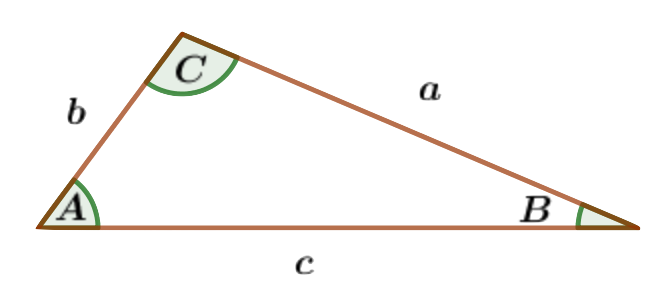
\includegraphics[width=0.45\textwidth]{img-triang/triang01.png}
\end{figure}
\end{multicols}



CLASIFICACION DE LOS TRIANGULOS

\underline{Según sus lados}:

\begin{itemize}
\item Equiláteros: sus tres lados son iguales y sus tres ángulos también por lo que $A+B+C=3\alpha=180^o \ \to \alpha=60^o$, los ángulos de un triángulo equilátero son de $60^o$ (equiangular).
\item Isósceles: dos lados iguales y uno desigual, cuyo ángulo opuesto es distinto de los otros dos (que también son iguales).
\item Escaleno: los tres lados desiguales (y también los tres ángulos).
\end{itemize}

\underline{Según sus ángulos}:
\begin{itemize}
\item T. Rectángulos: uno de sus ángulos es recto, es decir, mide 90$^o$.
\item T. Acutángulos: los tres ángulos interiores son agudos (menos de 90$^o$).
\item T. Obtusángulos: tienen un ángulo obtuso (más de 90$^p$).
\end{itemize}

\vspace{3mm}
TEST DE PITÁGORAS: sea $a$ el lado mayor o igual a los otros dos, $b$ y $c$, si

\hspace{2cm} $a^2\ < \ b^2+c^2 \ \to \ $ triángulo acutángulo.

\hspace{2cm} $a^2\ = \ b^2+c^2 \ \to \ $ triángulo rectángulo, ángulo recto $A$.

\hspace{2cm} $a^2\ > \ b^2+c^2 \ \to \ $ triángulo obtusángulo.


\vspace{4mm}
IMPORTANCIA DE LOS TRIANGULOS

Los triángulos tienen una importancia suprema en la geometría, pues todo polígono puede ser descompuesto o formado por triángulos. Esta gran importancia de los triángulos en la geometría, ya la conocían los geómetras desde los tiempos de las primeras civilizaciones.

El estudio tan amplio de los triángulos, que ha generado en sí misma una rama de la Geometría y de las Matemáticas, es la Trigonometría (medida de triángulos).

Si miras a tu alrededor encontrarás que el triángulo está presente en los puentes, en las grúas, etc. Es el polígono más sencillo y cualquier otro se puede descomponer en triángulos. El triángulo es muy utilizado en las estructuras porque es la única figura que no se puede deformar, hagas lo que hagas seguirá siendo un triángulo.

\vspace{5mm} \textsf{En lo sucesivo, consideraremos un triángulo cualquiera de ángulos A, B , C y lados opuestos a, b, c, respectivamente.}

\vspace{5mm}
\section{Teorema del coseno}

\begin{tikzpicture}
	\fill [left color=red!50, right color=teal!50] (0,0) rectangle (3.5,.1);
	\fill [left color=teal!50, right color=blue!50] (3.5,0) rectangle (7.5,.1);
	\end{tikzpicture}
\vspace{0.5cm}


\begin{theorem}[ Teorema del coseno]
	
	En cualquier triángulo se cumple que:
	
	$$\large{ \subrayado{ \boldsymbol{ \boxed{ \  a^2=b^2+c^2-2bc\cos A	\ } } } }$$
	
	\emph{En todo triángulo, el cuadrado de un lado siempre es igual a la suma de los cuadrados de los otros dos menos el doble producto de ellos por el coseno del ángulo comprendido.}
	
	$$\boldsymbol{ b^2=a^2+c^2-2ac\cos B \, ; \qquad \qquad c^2=a^2+b^2-2ab\cos C }$$
\end{theorem}

\underline{Demostración}:

\begin{multicols}{2}
\begin{figure}[H]
	\centering
	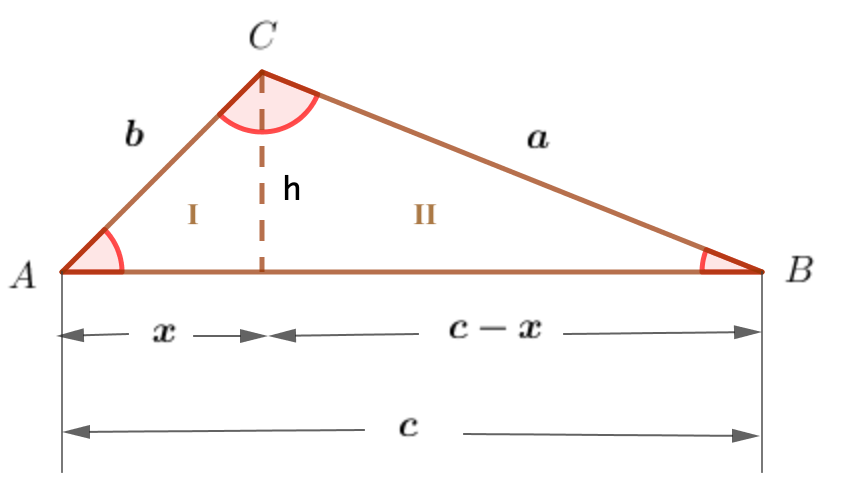
\includegraphics[width=0.45\textwidth]{img-triang/triang02.png}
\end{figure}
$I:\quad \ b^2=h^2+x^2$

$II:\quad a^2=h^2+(c-x)^2$

$I\to II:\quad a^2=(b^2-x^2)+(c-x)^2= $

$=b^2-\cancel{x^2}+c^2+\cancel{x^2}-2cx=b^2+c^2-2cx$

$I:\ \to \ \cos A=\dfrac x b \ \to \ x=b\cos A$

Luego: $\ a^2=b^2+c^2-2bc\cos A$ \QED	
\end{multicols}


\vspace{-3mm}

\underline{Observaciones} al teorema del coseno:

\begin{itemize}
\item En un triángulo rectángulo de hipotenusa $a \ \leftrightarrow \ A=90^o$, el teorema del coseno dice: $a^2=b^2+c^2-2bc \cancelto{0}{\cos 90}=b^2+c^2$, que no es más que el \emph{Teorema de Pitágoras}.
\end{itemize}

\vspace{-2mm}
\begin{multicols}{2}

\begin{itemize}
\vspace{-2mm}\item Al teorema del coseno también se le conoce como \emph{teorema de Pitágoras generalizado}.
\vspace{-2mm}\item \begin{small} Si se aplica el teorema del coseno a un cateto (por ejemplo $b$, siendo $a$ la hipotenusa) de un triángulo rectángulo, también se reproduce el teorema de Pitágoras (con el cateto despejado): 
$\ b^2=a^2+c^2-2ac\cos B=a^2+c^2-2ac  \dfrac{c}{a}=a^2+c^2-2c^2=a^2-c^2$ (constrúyase el dibujo adecuado).\end{small}
\end{itemize}

\begin{figure}[H]
	\centering
	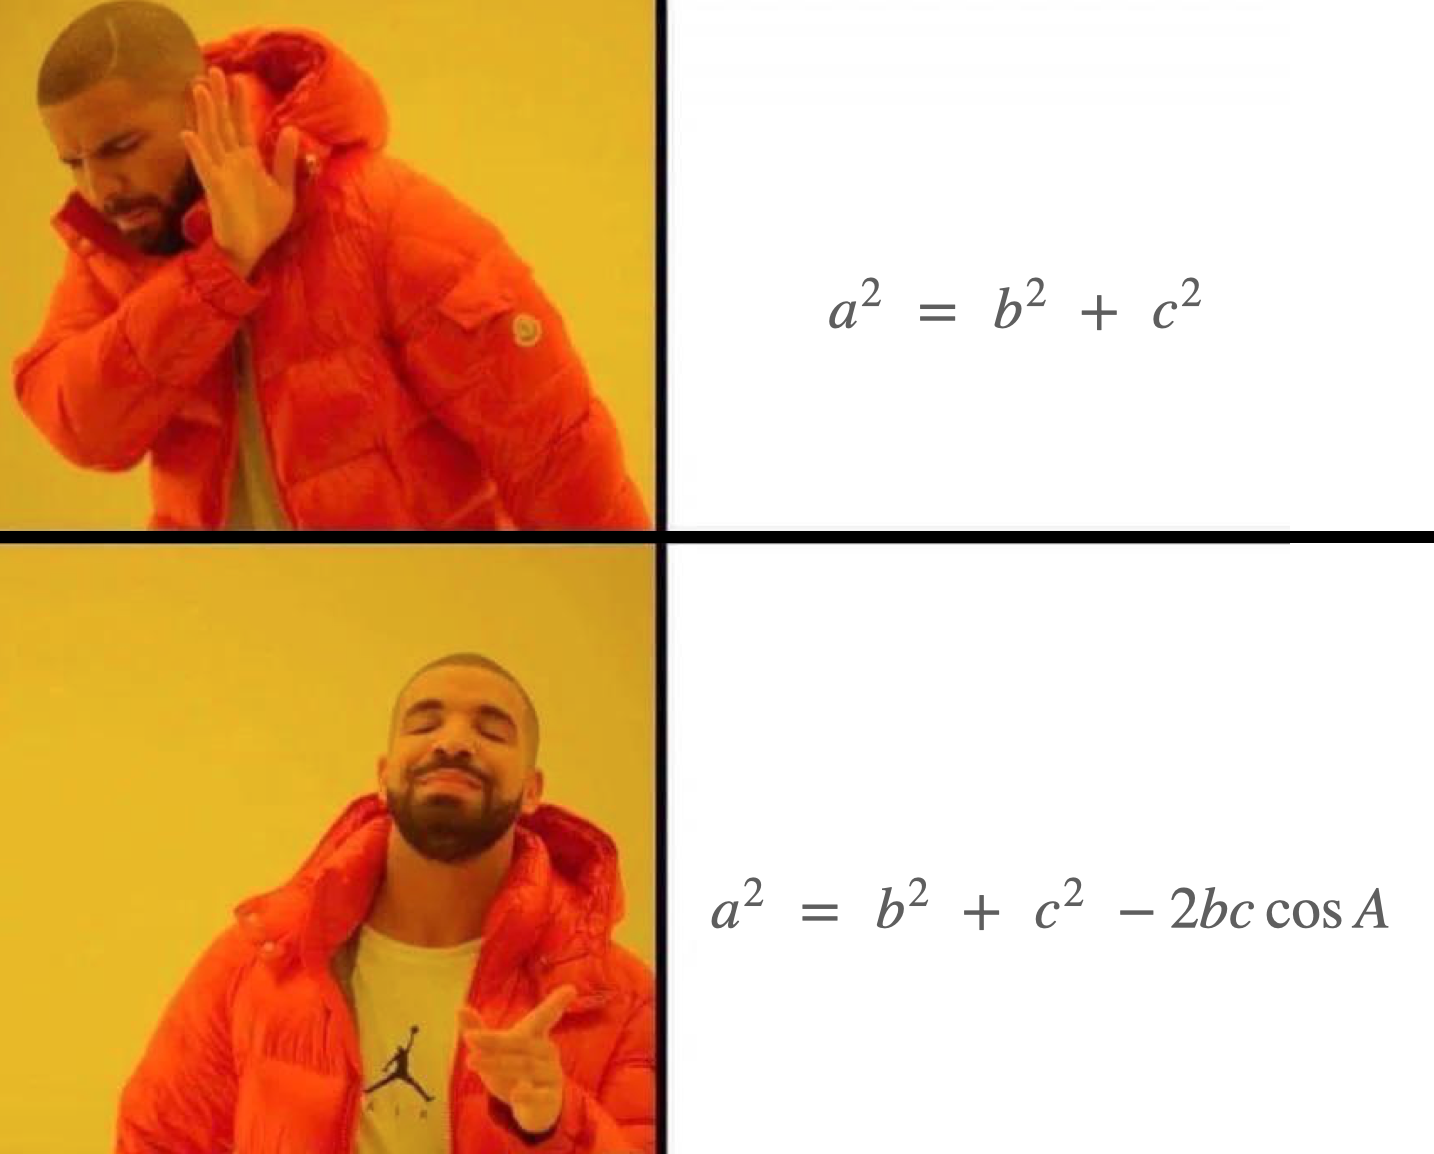
\includegraphics[width=0.4\textwidth]{img-triang/triang03.png}
\end{figure}

\end{multicols}

\begin{itemize}
\item Si el teorema de cosenos se aplica para calcular un ángulo se obtiene una solución única por ser los ángulos los de un triángulo, menores de 180$^o$.	
\end{itemize}


\begin{miejemplo}
	
	De un triángulo sabemos que $a=10\, \mathrm{u}$\footnote{$\ u$: unidades arbitrarias}, $b=7 \, \mathrm{u}$ y que $C=30^o$. Calcula el otro lado y los otros ángulos.

\vspace{5mm} Conocemos dos lados y el ángulo comprendido, por el teorema del coseno:

\vspace{2mm} $\triangleright \ \ c^2=a^2+b^2-2ab\cos C \ \Rightarrow \ c=\sqrt{10^2+7^2-2\cdot 10 \cdot 7\, \cos 30^o}=5.3 \, \mathrm{u}$.

\vspace{2mm} $\triangleright \ \ $ Por teorema de cosenos aplicado a otro lado, $\ a^2=b^2+c^2-2bc\cos A \ \to \ $

$cos A =  \dfrac{b^2+c^2-a^2}{2bc}  \ \Rightarrow \ A=\acos \left( \dfrac{7^2+5.3^2-10^2}{2\cdot 7 \cdot 5.3} \right)= 108.3^o$

\vspace{2mm} $\triangleright \ \ $ Finalmente, $B$ será el ángulo que falta hasta $180^o \ \Rightarrow \ B=180-108.3-30=41.7^o$
\end{miejemplo}

%%%%
\begin{miejercicio}

Los lados de un triángulo miden, 3, 4 y 5 u. Calcula sus ángulos.

\rule{250pt}{0.1pt}	

\vspace{4mm} $a=3\, \mathrm{u},\ b=4 \, \mathrm{u}, \ c=5 \, \mathrm{u}$

\vspace{2mm} $\triangleright \ $ Teorema cosenos: $a^2=b^2+c^2-2bc\cos A \ \to \ A=\acos \left( \dfrac{b^2+c^2-a^2}{2bc} \right) \ \Rightarrow \ A=\acos \dfrac{4^4+5^2-3^2}{2\cdot 4\cdot 5} = 36.87^o$

\vspace{2mm} $\triangleright \ $ Otra vez teorema cosenos: $c^2=a^2+b^2-2ab\cos C \ \to $

$\to \ \cos C= \dfrac{3^4+4^4-5^2}{2\cdot 3\cdot 4}= 0 \ \Rightarrow \ C = 90^o\ $ Triángulo rectángulo de hipotenusa $c=5 \, \mathrm{u}$

\vspace{2mm} $\triangleright \ $ El tercer ángulo será $B=180-36.87-90=53.13^o$
\end{miejercicio}



\vspace{5mm}
\section{Teorema del seno}

\begin{tikzpicture}
	\fill [left color=red!50, right color=teal!50] (0,0) rectangle (3.5,.1);
	\fill [left color=teal!50, right color=blue!50] (3.5,0) rectangle (7.5,.1);
	\end{tikzpicture}
\vspace{1cm}

\begin{theorem}[ Teorema del seno]

\emph{En todo triángulo el cociente entre un lado cualquiera y el seno de su ángulo opuesto es una constante, independientemente del lado elegido} \textcolor{gris}{que coincide con el diámetro de la circunferencia que circunscribe al triángulo.}

$$\subrayado{\boxed{\boldsymbol{\ \dfrac{a}{\sin A} \ = \  \dfrac{b}{\sin B} \ = \  \dfrac{c}{\sin D} \ }}}  = \  2R $$
	
\end{theorem}

\underline{Observaciones}:
\begin{itemize}
\item Realmente hay tres ecuaciones, una por cada dos lados y ángulos opuestos que escojamos de un triángulo.
\item Si se aplica el teorema del seno para conocer un lado de un triángulo no hay ningún problema, la solución es única. Pero ...
\item ... si se aplica el teorema del seno para calcular un ángulo de un triángulo hay dos soluciones, un ángulo agudo y uno obtuso. Esto no ocurre si se puede aplicar teorema de cosenos que proporciona una única solución para ángulos de triángulos (menores de 180$^o$).
\item Por este motivo, siempre que sea posible será aconsejable aplicar teorema de cosenos que de senos para el cálculo de un ángulo.  Si ello no es posible y hay que aplicar teorema de senos y se obtiene dos soluciones de la que si solo una de ellas es válida podemos usar que siempre, \emph{el lado más grande es el opuesto al ángulo más grande}, o mejor,  se puede hacer uso del \textbf{\emph{`test de Pitágoras'}}
\item \textcolor{gris}{Del teorema del seno es sencillo deducir que \emph{en todo triángulo, a mayor lado le corresponde mayor ángulo opuesto}, ya que el teorema asegura que su cociente es constante.}
\end{itemize}

%\vspace{5mm}
\underline{Demostración}:

\begin{figure}[H]
	\centering
	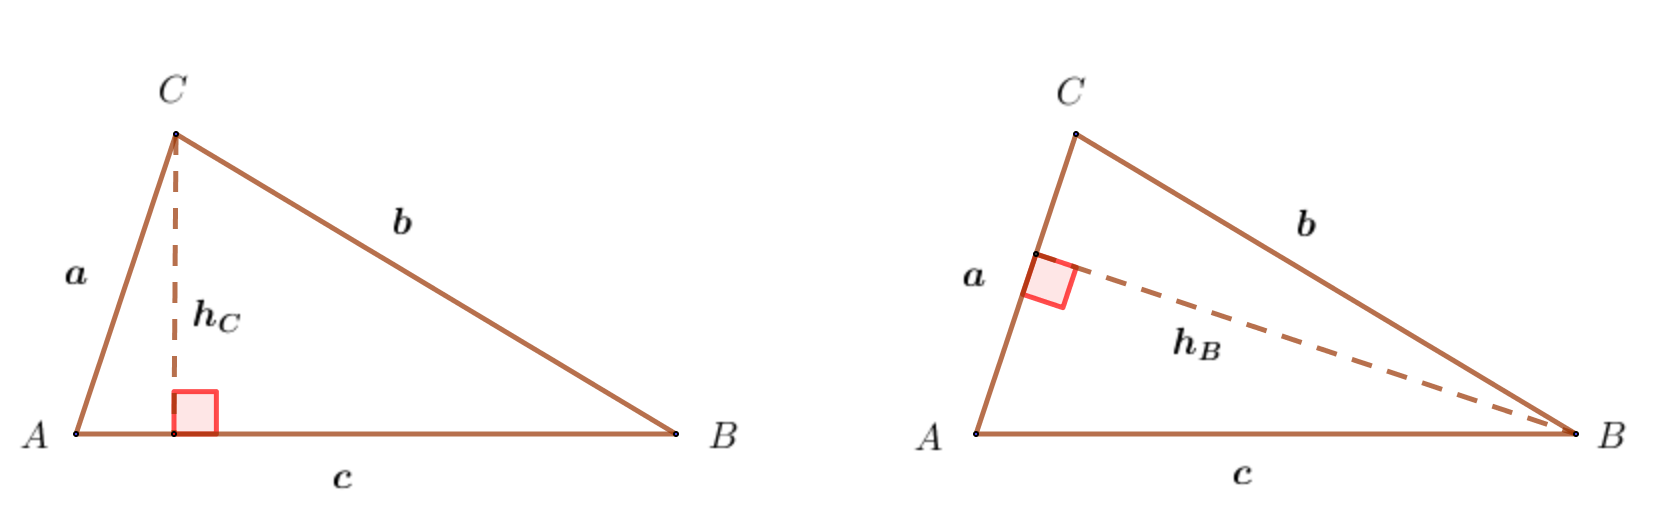
\includegraphics[width=0.75\textwidth]{img-triang/triang05.png}
\end{figure}

Altura de $C\, , \ h_C\, : \quad  \left. \mqty{ \sin A = \dfrac {h_C} b & \to & h_C=b\sin A & \ \\ \\ \sin B = \dfrac {h_C} a & \to & h_C=a\sin B &\  } \right\} \to \ b\sin A=a\sin B \ \Rightarrow \ \dfrac{a}{\sin A}=\dfrac{b}{\sin B}$

\vspace{2mm}
Altura de $B\, , \ h_B\, : \quad  \left. \mqty{ \sin A = \dfrac {h_B} c & \to & h_B=c\sin A & \ \\ \\ \sin C = \dfrac {h_B} a & \to & h_B=a\sin C &\  } \right\} \to \ c\sin A=a\sin C \ \Rightarrow \ \dfrac{a}{\sin A}=\dfrac{c}{\sin C}$

\vspace{2mm} Juntando ambos resultados, $\qquad  \dfrac{a}{\sin A} \ = \  \dfrac{b}{\sin B} \ = \  \dfrac{c}{\sin D}$\QED



\vspace{5mm}
\begin{myalertblock}{Teorema de senos y circunferencia circunscrita a un triángulo}

\emph{En un triángulo la razón, entre cada lado y el seno de su ángulo opuesto, es constante e igual al diámetro de la circunferencia circunscrita.}

\begin{multicols}{2}	
 $ABC$ triángulo circunscrito en la circunferencia de centro $\mathcal O$ y radio $R$. Aparecen tres triángulos $\mathcal OAB$, $\mathcal OAC$ y $\mathcal OBC$, todos ellos isósceles por lo que las alturas desde $\mathcal O$ caen todas en el punto medio de $a$, de $b$ y de $c$.

\vspace{4mm}Fijémonos en tres triángulos rectángulos (por construcción) que se forman, $B'\mathcal O C$, $A\mathcal O B$, $A'\mathcal O B$ y $C'\mathcal O A$ y en sus ángulos agudos respectivos $\beta$, $\alpha$ y $\gamma$.

	\begin{figure}[H]
	\centering
	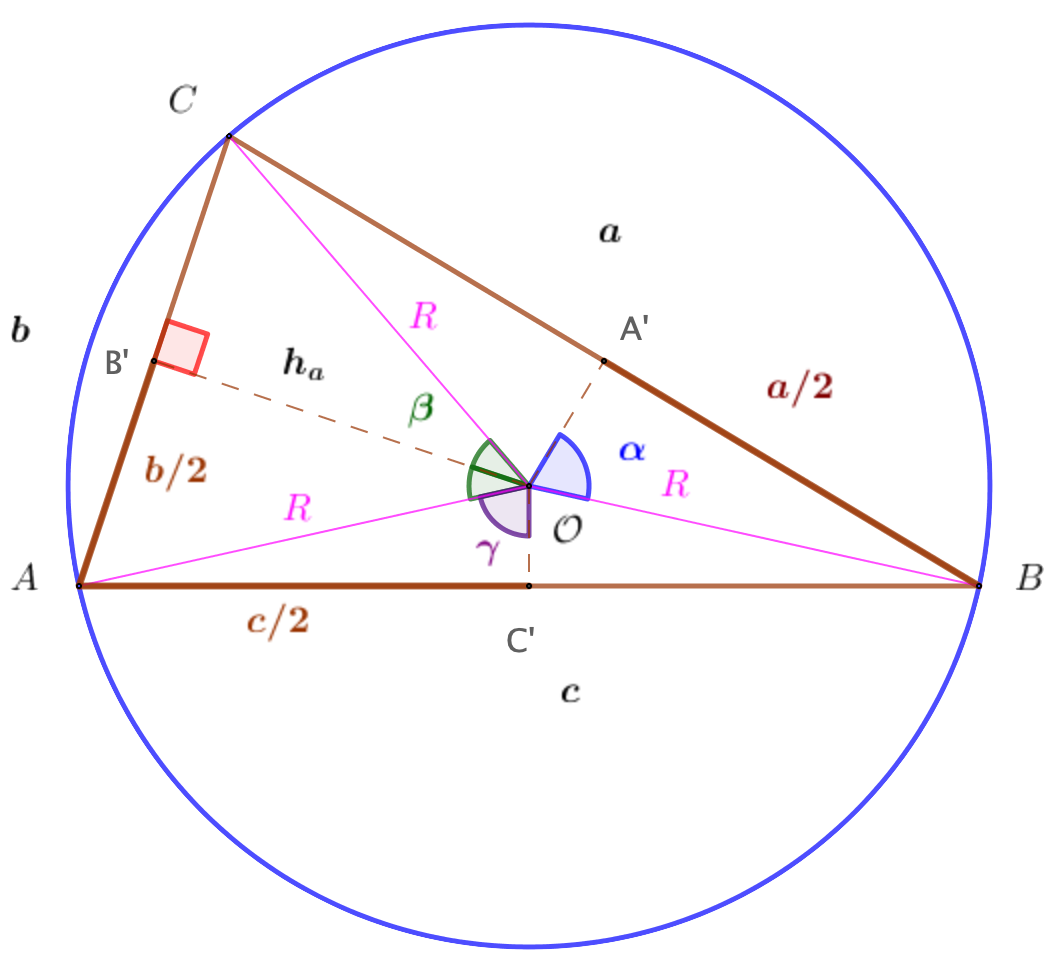
\includegraphics[width=0.5\textwidth]{img-triang/triang07.png}
\end{figure}
\end{multicols}
$\sin \alpha= \dfrac{a/2}{R} \ \to \ 2R=\dfrac{2}{\sin A} \ ; \ \quad \ \sin \beta= \dfrac{b/2}{R} \ ; \ \quad \ \sin \gamma=\dfrac{c/2}{R} \ \to \ 2R=\dfrac{c}{\sin \gamma} \ \to \ 2R=\dfrac{b}{\sin \beta}$

\vspace{2mm} Luego, $ \quad \dfrac{a}{\sin \alpha}=\dfrac{b}{\sin \beta}=\dfrac{c}{\sin \gamma}=2R \quad (*)$

\vspace{2mm} De la figura, $A=(180-90-\gamma)+(180-90+\beta)=180-\beta-\gamma \ \Rightarrow \ A+\beta+\gamma=180 \ (1*)$

\vspace{2mm} Análogamente se encuentra que $B=(180-90-\gamma)+(180-90-\alpha) \ \Rightarrow \ \alpha+B+\gamma=180 \ (2*)$ y también $\alpha+\beta+C=180 \ (3*)$. Como, por otro lado, del triángulo $ABC$ se cumple $A+B+C=180 \ (4*)$. Combinando estas cuatro expresiones llegaremos al resultado deseado:

\vspace{2mm} $(1)+(2*)-(3*)-(4*) \ \Rightarrow \ 2A-2\alpha=0 \ \to \ A=\alpha;\quad (1)-(2*)+(3*)-(4*) \ \Rightarrow \ B=\beta \ \text{ y } \ (1)-(2*)-(3*)+(4*) \ \Rightarrow \ C=\gamma\ $ Llevando estos resultados a (*):

\begin{multicols}{2}
	\begin{center} $ \dfrac{a}{\sin A} \ = \  \dfrac{b}{\sin B} \ = \  \dfrac{c}{\sin D} \ = \ 2R $  \end{center} \QED
\end{multicols}
\vspace{-3mm}

\begin{center}\rule{250pt}{0.1pt} \end{center}

\begin{small}
\underline{Otra demostración} más rápida:

\begin{multicols}{2}
Dado el triángulo $ABC$ inscrito en la circunferencia, trazamos desde $B$ un diámetro $BD$.

Los ángulos $\widehat{BDC}=\widehat{BAC}=A$ son iguales por tratarse de ángulos inscritos en una circunferencia que abarca el mismo arco 
$\stackrel{\textstyle\frown}{BC}\, , \  $ además, el triángulo $BCD$ es rectángulo en $C$ (ángulo central 180$^o$, ángulo inscrito 90$^o$) , por lo que:

$\quad  \sin A=\dfrac {2}{2R} \ \to \ \boldsymbol{ \dfrac{a}{\sin A}\ = \ 2R } $

Del mismo modo con los otros pares lado-ángulo opuesto. \QED
\begin{figure}[H]
	\centering
	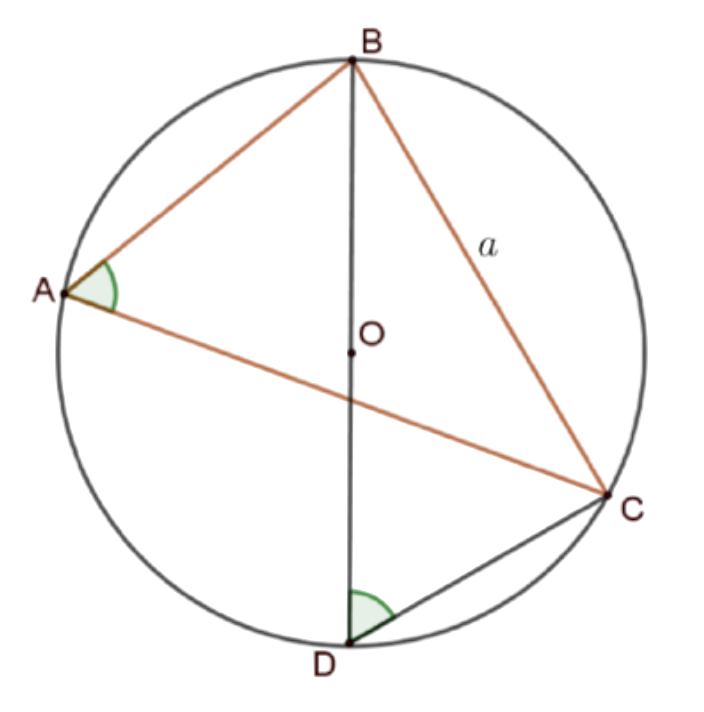
\includegraphics[width=0.3\textwidth]{img-triang/triang08.png}
\end{figure}	

\end{multicols}

\end{small}
\end{myalertblock}

\begin{miejemplo}

Conocidos $a=7.5\, \mathrm{cm}$ , $b=8\, \mathrm{cm}$ y el ángulo $B=50^o$, calcula el lado  y los ángulos que faltan.

\vspace{5mm} Por teorema de senos: $\quad \dfrac{a}{\sin A}=\dfrac{b}{\sin B} \ \to \ \sin A=\dfrac{a\sin B}{b}=\dfrac{7.5\cdot \sin 50}{8} \ \to $

\vspace{2mm} $\to \begin{cases} \ \boldsymbol{ A= 46^o} &\to  \boldsymbol C=180-A-B= \boldsymbol{ 84^o} \\ \ A=134^o &\to \nexists C \end{cases}$

\vspace{2mm} Finalmente, $\quad \dfrac{a}{\sin A}=\dfrac{c}{\sin C } \ \to \ \boldsymbol c=\ \dfrac{a\sin C}{\sin A}=\dfrac{7.5\cdot \sin 84}{\sin 46}=\ \boldsymbol{ 10.4 \,\mathrm{cm} }$
\end{miejemplo} 

\begin{miejercicio}

Conocidos $c=3\, \mathrm{m}$ , $b=2\, \mathrm{m}$ y el ángulo $B=30^o$, calcula el lado  y los ángulos que faltan.

\rule{250pt}{0.1pt}

\vspace{2mm} Teorema de senos: $\quad \dfrac{b}{\sin B}=\dfrac{c}{\sin C} \ \to \ \sin C=\dfrac{c\sin B}{b}=\dfrac{3\cdot \sin 30}{2}=0.75 \to $

\vspace{2mm}  $\to C=\asin 0.75 = \begin{cases} \ C= 48.6^o  \\ \ C=131.4^o \end{cases} \ \to  A=180-C-B \ \begin{cases} 
\ A=101.4^o &\to  \text{ Trian. I} \\  
\ A=18.6^o  &\to  \text{ Trian. II} 
\end{cases} \ \to $

\vspace{2mm}  $\to \   \dfrac{a}{\sin A}=\dfrac{b}{\sin B} \ \to \ a=\dfrac{b\sin A}{\sin B} \ \to 
\begin{cases}
\ a=\dfrac{2\cdot \sin 101.4}{\sin 30 } &\to a=3.92 \, \mathrm{m} \\ 	
\ a=\dfrac{2\cdot \sin 18.6}{\sin 30 } &\to a=1.28 \, \mathrm{m} 
\end{cases}$
 
\vspace{4mm}  Hay dos soluciones: $\quad $ Triángulo I: $\ A=101.4^o,\ B=30^o, \ C= 48.6^o ; \ a=3.92 \, \mathrm{m} ,\ b= 2\, \mathrm{m} , º c=3 \, \mathrm{m} $ y el triángulo II:  $\ A=18.6^o,\ B=30^o, \ C= 131.4^o ; \ a=1.28 \, \mathrm{m} ,\ b= 2\, \mathrm{m} , º c=3 \, \mathrm{m} $

\vspace{2mm} \textcolor{gris}{Para dibujar los dos triángulos partimos de dibujar $c=AB=3\, \mathrm{u}$ y en $B$ dibujamos la recta $r$ que forma un ángulo de $30^o$ con $c$. Desde $A$ trazamos una circunferencia de radio $a=2 \, \mathrm{u}$. Las intersecciones de la circunferencia con la recia $r$ nos dan los dos posibles vértices de los triángulos buscado, $C_1$ y $C_2$}
\begin{figure}[H]
	\centering
	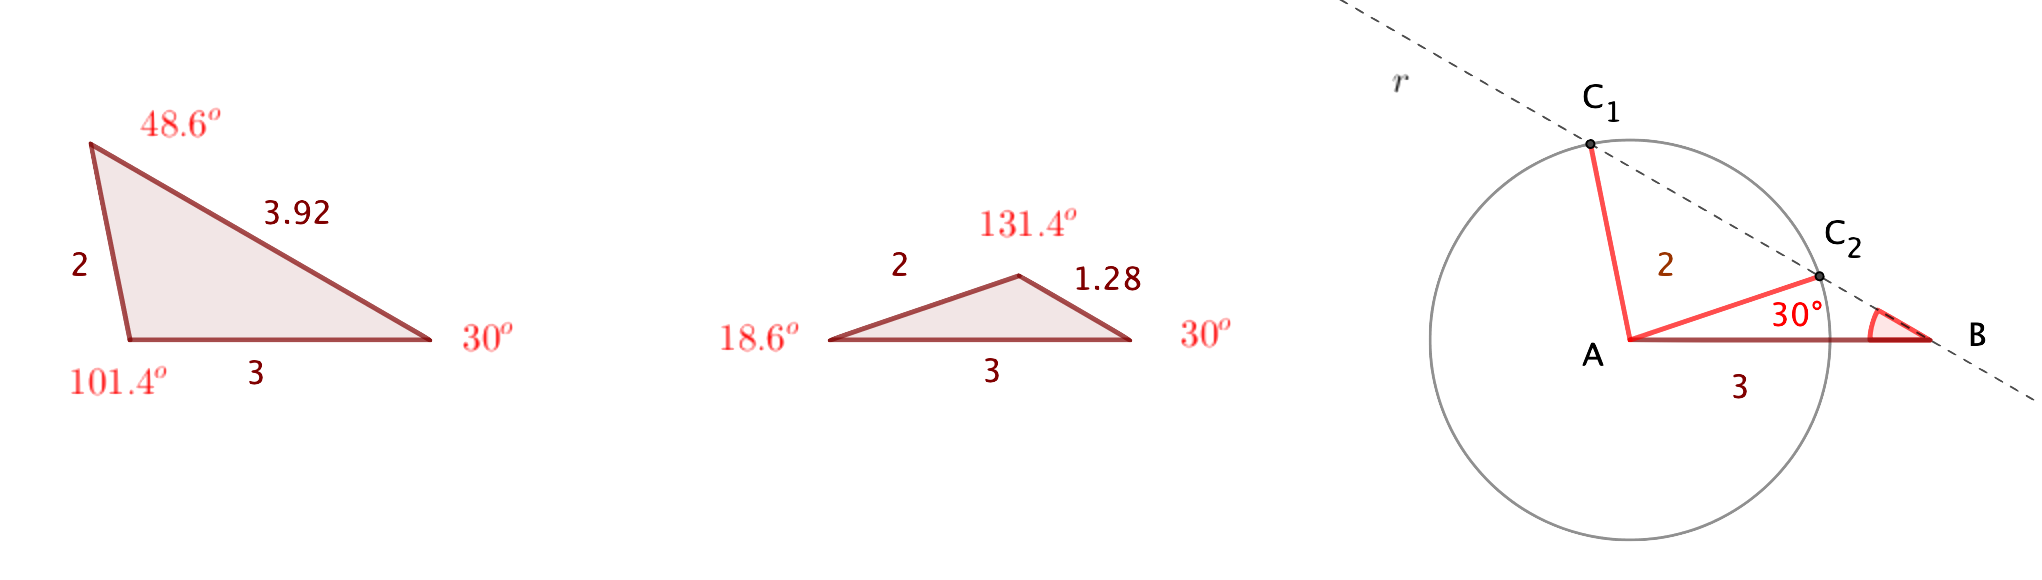
\includegraphics[width=1\textwidth]{img-triang/triang10.png}
\end{figure}
	
\end{miejercicio}

\begin{miejercicio}

Dado el triángulo $a=100 \, \mathrm{cm},\ b=185 \,  \mathrm{cm},\ c= 150 \,  \mathrm{cm}\, , $ encuentra cuales son sus ángulos.

\rule{250pt}{0.1pt}

\vspace{2mm} Dados tres lados que puedan formar un triángulo \textcolor{gris}{(en todo triángulo, un lado es menor que la suma de los otros dos y mayor que su diferencia)}, existirá una única solución; solo se tiene que construir los tres segmentos e intentar encajarlos formando un triángulo: si existe, la solución será única. Vamos a resolver el problema por dos métodos:

\vspace{2mm} MÉTODO I: aplicaremos el teorema de cosenos dos veces para encontrar dos de los tres ángulos, el tercero será el necesario para que entre los tres sumen 180$^o$.

\vspace{2mm} MÉTODO II: aplicaremos una vez el teorema de cosenos para calcular un ángulo y el teorema de senos para calcular otro (ojo, al aplicar teorema de senos para el cálculo de un ángulo puede haber dos soluciones). El tercer ángulo será el necesario para que entre los tres sumen 180$^o$.

\vspace{4mm} $\triangleright \ \ $ \underline{Método I}: 

\vspace{2mm} $a^2=b^2+c^2-2bc\cos A\ \to \ \cos A=\dfrac{b^2+c^2-a^2}{2bc}=\dfrac{185^2+150^2-100^2}{2\cdot 185\cdot 150} \ \to  A=32.66^o$

\vspace{2mm} $b^2=a^2+c^2-2ac\cos B\ \to \ \cos B=\dfrac{a^2+c^2-b^2}{2ac}=\dfrac{100^2+150^2-185^2}{2\cdot 100\cdot 150} \ \to  B=93.30^o$

\vspace{2mm} $A+B+C=180^o \ \to \ C=180-A-B=180-32,66-93.30 \ \to \ C=54.04^o$

\vspace{2mm} La solución es, evidentemente, única.


\vspace{4mm} $\triangleright \ \ $ \underline{Método II}: 

\vspace{2mm} $a^2=b^2+c^2-2bc\cos A\ \to \ \cos A=\dfrac{b^2+c^2-a^2}{2bc}=\dfrac{185^2+150^2-100^2}{2\cdot 185\cdot 150} \ \to  A=32.66^o$

\vspace{2mm} $\dfrac{a}{\sin A}=\dfrac{b}{\sin B} \ \to \ \sin B=\dfrac{b\sin A}{a}=\dfrac{185 \, \sin 32.66}{100} \ \to $

\vspace{2mm}$\to \ \begin{cases}
 	\ B_1=86.72^o &\to C_1=180-A-B_1=60.22^o \ \text{ sol I} \\
 	\ B_2=180-86.72=93.28^o &\to C_2=180-A-B_2=54.06^o \ \text{ sol II} 
 \end{cases}$

\vspace{2mm} \emph{!`Extraño, no puede ser, dados tres lados la soluuión ha de ser única!}

\vspace{2mm} Para discenir cuál de los dos soluciones es la correcta recurriremos al test de Pitágoras. Como el lado mayor es $b$, comparamos $b^2$ con $a^2+c^2$:

\vspace{2mm} $b^2=185^2=34225 \ \boldsymbol{>} \ 32500=100^2+150^2=a^2+c^2 \ \Rightarrow \ $ el triángulo es obtusángulo en $B$

\vspace{2mm} La solución correcta es la II, $\ A=32.66^o,\ B=93.28^o,\ C=54.06^o$, tal y como habíamos obtenido en el método-I.

\begin{multicols}{2}
\begin{footnotesize} Construcción del triángulo:
dibujamos $b$ como base. Con centro en $C$ dibujamos una circunferencia de radio $a=100$, con centro en $A$ dibujamos una circunferencia de radio $c=150$.

La intersección de ambas circunferencias nos da la posición del tercer vértices $B$.\textcolor{gris}{Realmente no hay dos soluciones, la intersección inferior de las circunferencias da lugar al mismo triángulo (simétricos respecto de las bases $b$)}\end{footnotesize}
\begin{figure}[H]
	\centering
	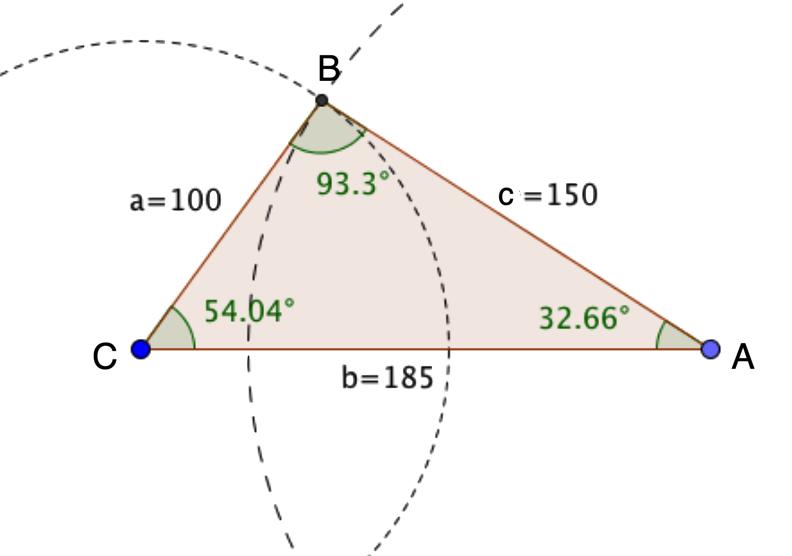
\includegraphics[width=.4\textwidth]{img-triang/triang11.png}
\end{figure}	
\end{multicols}	
\end{miejercicio}

\vspace{5mm} 


\subsection{Teorema de la tangente}
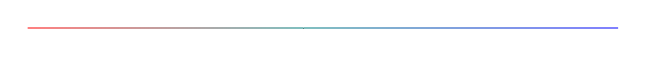
\begin{tikzpicture}
	\fill [left color=red!50, right color=teal!50] (0,0) rectangle (3.5,.01);
	\fill [left color=teal!50, right color=blue!50] (3.5,0) rectangle (7.5,.01);
	\end{tikzpicture}
\vspace{0.2cm}


\begin{myexampleblock}{Teorema de las tangentes}


\begin{theorem} [ Teorema de las tangentes]
	
El teorema de la tangente relaciona las longitudes de dos lados de un triángulo con las tangentes de los dos ángulos opuestos a éstos.

\begin{multicols}{2}
Para cada dos lados cualesquiera de un triángulo, $a,\ b$ por ejemplo, y para sus ángulos opuestos correspondientes, $A,\ B$, se cumple:

$$\boldsymbol{ \dfrac{a+b}{a-b} \ = \ \dfrac{ \tan \left( \dfrac{A+B}{2} \right) }{  \tan \left( \dfrac{A-B}{2} \right) } }\, ; \ \ \  \qquad 
\dfrac{a+c}{a-c} \ = \ \dfrac{ \tan \left( \dfrac{A+C}{2} \right) }{  \tan \left( \dfrac{A-C}{2} \right) }  \, ; \qquad
\dfrac{b+c}{b-c} \ = \ \dfrac{ \tan \left( \dfrac{B+C}{2} \right) }{  \tan \left( \dfrac{B-C}{2} \right) }  
$$

\begin{figure}[H]
	\centering
	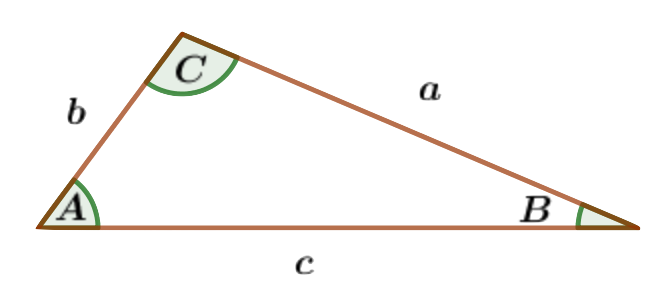
\includegraphics[width=.4\textwidth]{img-triang/triang01.png}
\end{figure}	
\end{multicols}
\end{theorem}


\underline{Demostración}: nos basamos en el teorema de senos y en la transformación en productos.

\vspace{2mm} $\dfrac{a}{\sin A}=\dfrac{b}{\sin B}=\text{constante}=x \ \to \ \begin{cases} \ a=x\sin A \\ \ b=x\sin B \end{cases}$

\vspace{2mm} $\dfrac{a+b}{a-b}=\dfrac{x\sin A+ x\sin B}{x\sin A-x\sin B}=\dfrac{\sin A+ \sin B}{\sin A-\sin B}=\dfrac{\cancel{2}\ \sin \left( \dfrac{A+B}{2} \right) \ \cancel{ \cos \left( \dfrac{A-B}{2} \right)  } } 
{\cancel{2}\ \cos \left( \dfrac{A+B}{2} \right) \ \cancel{ \cos \left( \dfrac{A-B}{2} \right)  } } = 
\dfrac{ \tan \left( \dfrac{A+B}{2} \right) }{  \tan \left( \dfrac{A-B}{2} \right) }$ \QED


\vspace{2mm} \underline{Aplicaciones}: resolución de triángulos en que se conocen dos lados y un ángulo o un lado y dos ángulos.

\vspace{2mm}
\begin{footnotesize}
\begin{miejemplo}

Encuentra los datos que faltan en el triángulo $\ a=4.2\, \mathrm{u}\, , \ b=3.8\, \mathrm{u} \, , \ C=60^o$

\vspace{4mm} $A+B+C=180 ,\ C=60 º \to \ A+B=180-60=120$

\vspace{2mm} $\dfrac{4.2+3.8}{4.2-3.8} \ = \ \dfrac{a+b}{a-b} \ = \ \dfrac{ \tan \left( \dfrac{A+B}{2} \right) }{  \tan \left( \dfrac{A-B}{2} \right) }\ = \ \dfrac{\tan 60 }{ \tan \left( \dfrac{A-B}{2} \right) } \ \to \ $

\vspace{2mm} $\to \ \tan \left( \dfrac{A-B}{2} \right)=0.0866 \ \to \ \dfrac{A-B}{2}=4.94^o \ \to \ A-B=9.9^o \ \Rightarrow$

\vspace{2mm}$\Rightarrow \ \begin{cases}
 	\ A+B=120 \\ \ A-B=9.9 
 \end{cases} \ \to \ A=64.95^o \ \wedge \ B=55.05^o$

\vspace{2mm}  Por teorema de senos, ahora, $\ \dfrac{a}{\sin A}=\dfrac{c}{\sin C} \ \to \ c=\dfrac{a\sin C}{\sin A}=\dfrac{4.2\, \sin 60}{\sin 64.95}= 4.02\, \mathrm{u}$		
\end{miejemplo}
\end{footnotesize}

\end{myexampleblock}

\vspace{5mm}
\section{Área de un triángulo}
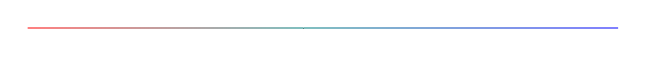
\begin{tikzpicture}
	\fill [left color=red!50, right color=teal!50] (0,0) rectangle (3.5,.01);
	\fill [left color=teal!50, right color=blue!50] (3.5,0) rectangle (7.5,.01);
	\end{tikzpicture}
\vspace{5mm}


El área de un triángulo es la mitad del producto de la base por la altura.

\vspace{4mm}
\begin{theorem}[ Área de un triángulo]

$$\boldsymbol{ 
	\subrayado{ \ \boxed{ \ 
\mathcal A \ = \ \dfrac 1 2 \, a\, b\, \sin C\,
\ } \ } ; \qquad 
\subrayado{ \ \boxed{ \ \mathcal A \ = \ \dfrac 1 2 \, a\, c\, \sin B \, \ } \ } ;\qquad 
\subrayado{ \ \boxed{ \ \mathcal A\ = \ \dfrac 1 2 \, b\, c\, \sin A \ } \ } }$$

\emph{El área de un triángulo es la mitad del producto de dos de sus lados por el seno del ángulo comprendido.}
\end{theorem}



\vspace{2mm} \underline{Demostración}:

\begin{multicols}{2}
Supuesto el triángulo apoyado en $c$, trazamos su altura $h$, así $\ \mathcal A=\dfrac 1 2 c h$

Pero, $\ h=b\sin A \ \to \ \mathcal A=\dfrac 1 2 \, c\,  b \sin A$

Y también, $\ h=a\sin B \ \to \ \mathcal A=\dfrac 1 2 \, c \, a \sin B$

\begin{figure}[H]
	\centering
	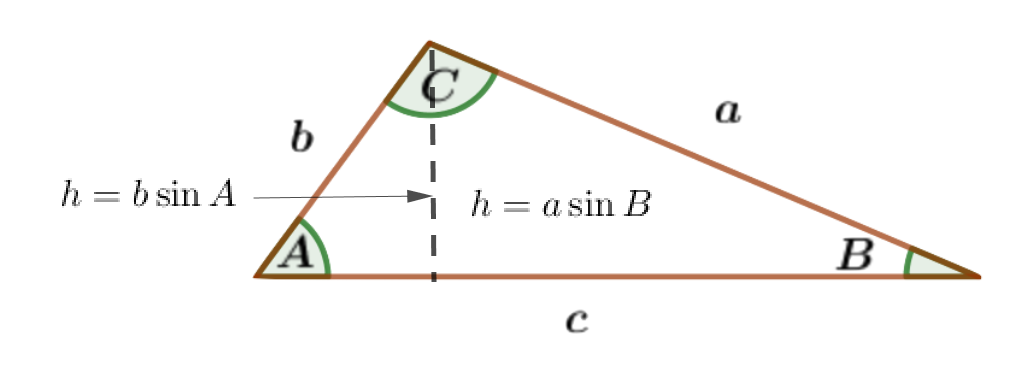
\includegraphics[width=.5\textwidth]{img-triang/triang12.png}
\end{figure}	
\end{multicols}
Apoyado el triángulo en cualquier otro lado, obtenemos la fórmula que nos falta. \QED


\vspace{5mm}

\begin{myalertblock}{Fórmula de Herón para el cálculo del área de un triángulo}

\vspace{2mm} Herón de Alejandría (siglo III a. de C). Su fórmula nos permite calcular el área de un triángulo conocidos los tres lados. No es necesario por tanto conocer la altura ni ninguno de los ángulos. Si llamamos $p$ al semiperímetro y $a$, $b$, $c$ a los tres lados, es decir,
$\ p=\dfrac{a+b+c}{2}$, el área se puede escribir como:


$$\large{ \boxed{ \  \boldsymbol{\mathcal A \ = \ \sqrt{\, p\, (p-a)\, (p-b)\, (p-c)\, }} \ } }$$

\vspace{2mm} La demostración se basa en el teorema del coseno.

\begin{multicols}{2}
\begin{figure}[H]
	\centering
	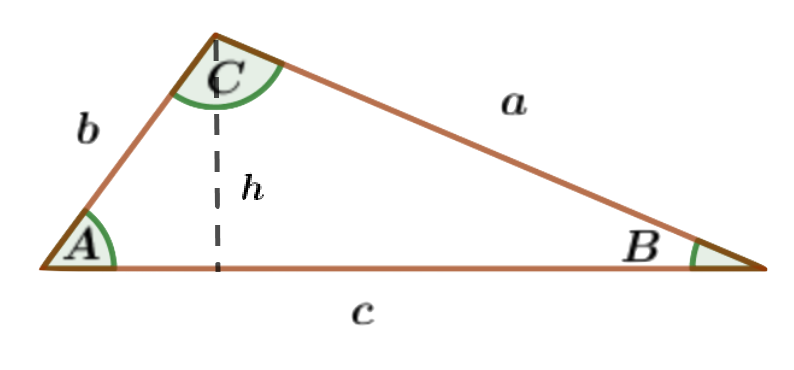
\includegraphics[width=.4\textwidth]{img-triang/triang13.png}
\end{figure}

$\quad$ $\mathcal A \ = \ \dfrac{c\cdot h}{2}\ = \ \dfrac{c\, a\, \sin B}{2}$

\vspace{2mm}$\quad$  Por teorema del coseno, 

\vspace{2mm}$\quad$  $b^2=a*2+c^2-2ac\cos B$	
\end{multicols}
\vspace{-4mm} Despejaremos $\cos B$ y sustituiremos en la expresión encontrada para  $\mathcal A$

\vspace{2mm} $\cos B=\dfrac{a^2+c^2-b^2}{2ac}\quad \to \quad \sin B=\sqrt{1-\cos^2 B} =\sqrt{1-\dfrac{(a^2+c^2-b^2)^2}{4a^2c^2}}$

\vspace{2mm}$\sin B=\sqrt{\dfrac{4a^2c^2-(a^2+c^2-b^2)^2}{4a^2c^2}}\quad $ Escribimos el numerador como  suma por diferencia,

\vspace{2mm} $\sin B=\dfrac{\sqrt{[2ac+(a^2+c^2-b^2)]\, [2ac-(a^2+c^2-b^2)]}}{2ac} = \dfrac{\sqrt{[(a+c)^2-b^2]\,[b^2-(a-c)^2]}}{2ac}$

\vspace{2mm} Sustituyendo en la fórmula del área, $\quad \mathcal A=\dfrac{ca}{2} \, \dfrac{\sqrt{[(a+c)^2-b^2]\,[b^2-(a-c)^2]}}{2ac} =$

\vspace{2mm} $\mathcal A=  \dfrac{\sqrt{[(a+c)^2-b^2]\,[b^2-(a-c)^2]}}{4}\quad$ De nuevo, escribimos como sumas por diferencias,

\vspace{2mm}  $\mathcal A=  \dfrac{\sqrt{(a+c+b)(a+c-b)\, (b+a-c)(b-a+c)}}{4}$

\vspace{2mm} Introduciendo el $4$ dentro de la raiz y observando que $\ \dfrac{b+a-c}{2}=\dfrac{p-c}{2},\ \ \dfrac{b-a+c}{2}=\dfrac{p-a}{2},\ \ \dfrac{a+c-b}{2}=\dfrac{p-b}{2}   \ \text{ y } \   \dfrac{a+b+c}{2}=\dfrac{p}{2}\, , \ $ obtenemos, finalmente,

\vspace{2mm} $\mathcal A \ = \ \sqrt{\, p\, (p-a)\, (p-b)\, (p-c)\, }$ \QED

\vspace{1mm}	
\end{myalertblock}

\vspace{4mm}

\begin{miejemplo}
	
	Los lados de un triángulo miden, $a=3 \, \mathrm{km}$, $b=4\,  \mathrm{km}$ y $c=5\,  \mathrm{km}$. Calcula su área.
	
\vspace{4mm} $\triangleright \quad $ por teorema de cosenos	calculamos un ángulo: $\quad a^2=b^2+c^2-2bc\cos A \ \to \ $

\vspace{3mm} $\to \ \cos A=\dfrac{b^2+c^2-a^2}{2bc}=\dfrac{4^2+5^5-3^2}{2\cdot 4\cdot 5 } \ \to \ A=36.87^o$

\vspace{2mm} Fórmula del área, $\quad \mathcal A=\dfrac 1 2\, b\, c\, \sin A=\dfrac 1 2 \, 4\cdot 5\cdot \sin 36.87 = 6\, \mathrm{km}^2$

\vspace{4mm} Por el teorema de Herón, $p=(a+b+c)/2=(3+4+5)/2=6\, \mathrm{km}$

\vspace{2mm} $\mathcal A=\sqrt{6(6-3)(6-4)(6-5)}=\sqrt{6\cdot 3\cdot 2 \cdot 1}=	\sqrt{36}=6\, \mathrm{km}^2$
\end{miejemplo}





\vspace{5mm}
\section{Resolución de triángulos}

\begin{tikzpicture}
	\fill [left color=red!50, right color=teal!50] (0,0) rectangle (3.5,.1);
	\fill [left color=teal!50, right color=blue!50] (3.5,0) rectangle (7.5,.1);
	\end{tikzpicture}
\vspace{1cm}

\begin{definition}[ ?`Qué es resolver un triángulo?]

Resolver un triángulo es es uno de los principales problemas de los que se ocupa la trigonometría. Consiste en determinar las dimensiones características de un triángulo. Para ello serán necesarios, al menos, tres datos siendo como mínimo uno de ellos un lado (dados tres ángulos que puedan formar un triángulo, suma menor que $\pi$, existen infinitas soluciones). 

\vspace{2mm} Resolver un triángulo es pues conocer sus tres lados y sus tres ángulos (y, para algunos autores, el área).
	
\end{definition}




\vspace{5mm}Puesto que para resolver un triángulo se necesitan tres datos y que al menos uno de ellos sea un lado, se presentarán los siguientes \underline{casos}:

\begin{enumerate}[i) ]
\vspace{-2mm} \item Conocidos un lado y dos ángulos.
\vspace{-2mm} \item Conocidos dos lados y el ángulo comprendido entre ellos.
\vspace{-2mm} \item Conocidos dos lados y un ángulo no comprendido entre ellos.
\vspace{-2mm} \item Conocidos los tres lados.	
\end{enumerate}

Para ello disponemos de las siguientes herramientas matemáticas:

\begin{itemize}
\vspace{-2mm} \item Teorema de senos.
\vspace{-2mm} \item Teorema de cosenos.
\vspace{-2mm} \item La suma de los ángulos de un triángulo es 180$^o$ \textcolor{gris}{(test de Pitágoras)}.	
\vspace{-2mm} \item Fórmulas para el área del triángulo.
\end{itemize}


\underline{Notación}: en esta sección llamaremos $\alpha$ al ángulo del vértice A, $\beta$ al de $B$ y $\gamma$ al de $C$.\footnote{ Las figuras de este apartado son de wikipedia}


\vspace{0.3cm}
\begin{multicols}{2}

	\textbf{I) Un lado y dos ángulos}
	
	Datos \textcolor{blue}{$c, \ \alpha, \ \beta\, . \ $} Incógnitas \textcolor{red}{$\ a,\ b,\ \gamma$}
	
	Condición: $\alpha+\beta<180^o \ \to \ $ solución única.
	
	$\triangleright \quad  \gamma=180-\alpha-\ beta$
	
	$\triangleright \quad  a \text{ y } b \ $ aplicando dos veces el teorema de senos.
	
	\begin{figure}[H]
		\centering
		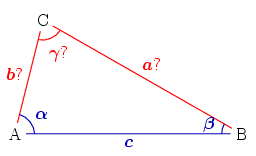
\includegraphics[width=.45\textwidth]{img-triang/RTC1.png}
	\end{figure}	
\end{multicols}


\vspace{0.3cm}
\begin{multicols}{2}
\textbf{II) Dos lados y ángulo comprendido}

Datos \textcolor{blue}{$a,\ b,\ \gamma\, . \ $} Incógnitas \textcolor{red}{$\alpha, \ \beta, \ c$}

Siempre solución única.

$\triangleright \quad c$ por teorema de cosenos.

$\triangleright \quad \alpha \ \vee \ \beta$ por teorema de cosenos, el otro ángulo ($\beta \ \vee  \ \alpha$) será lo que falte para que entre los tres sumen 180$^o$.
\begin{figure}[H]
	\centering
	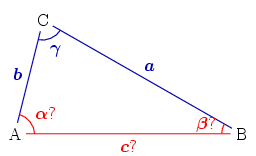
\includegraphics[width=.45\textwidth]{img-triang/RTC2.png}
\end{figure}	
\end{multicols}



\vspace{0.4cm}
\textbf{III) Dos lados y ángulo no comprendido}
\begin{multicols}{2}

Datos \textcolor{blue}{$b,\ c, \ \beta \, . \ $} Incógnitas \textcolor{red}{$a,\ \alpha, \ \gamma$}

$\triangleright \quad \gamma$ por teorema de senos:

si $\sin \gamma>1$, no hay solución; si $\sin \gamma=1$, la solución es un único triángulo rectángulo; si $\sin \gamma<1$ puede haber una o dos soluciones.

$\triangleright \quad \alpha$ lo que falte hasta 180$^o$. 

$\triangleright \quad a$ por teorema de senos. 

\begin{figure}[H]
	\centering
	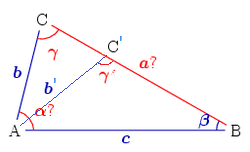
\includegraphics[width=.45\textwidth]{img-triang/RTC3.png}
\end{figure}	
\end{multicols}

\begin{small}
\textsf{Hay otra forma de proceder en este caso: aplicamos teorema del coseno para el ángulo del dato. El tercer lado que buscamos aparecerá como una incógnita en una ecuación de segundo grado:}

\vspace{-2mm} \begin{itemize}
\vspace{-2mm} \item \textsf{si no hay solución, el triángulo no tiene solución.}	
\vspace{-2mm} \item \textsf{si hay una sola solución, procedemos resolviendo el problema.}
\vspace{-2mm} \item \textsf{si hay dos soluciones, resolvemos para cada una de ellas y se obtendrán dos triángulos.}
\end{itemize}
\vspace{-2mm} \textsf{Cuando conozcamos los tres lados y un ángulo, para calcular otro ángulo por teorema de senos lo haremos siempre con el lado menor, así encontraremos el posible ángulo obtuso. (Ver ejercicio resuelto 8.8)} \end{small}


\vspace{0.4cm}

\begin{multicols}{2}
\textbf{IV) Tres lados}

Condición: la suma de dos cualesquiera de los lados ha de ser mayor que el tercero.

Datos \textcolor{blue}{$ a,\ b,\c \, . \ $} Incógnitas \textcolor{red}{$ \alpha,\ \beta,\ \gamma $}

$\triangleright \quad $ Aplicando dos veces el teorema de cosenos caslculamos dos ángulos, por ejemplo $\alpha \text{ y } \beta$

$\triangleright \quad $ $\gamma$ será lo que falte hasta 180$^o$ a la suma de los dos anteriores.

\begin{figure}[H]
	\centering
	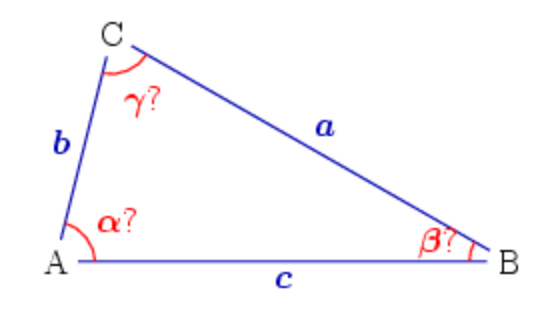
\includegraphics[width=.45\textwidth]{img-triang/RTC4.png}
\end{figure}
\end{multicols}


\vspace{5mm}


\begin{miejercicio}

Resuelve el siguiente triángulo: $\quad a=56 \, \mathrm{u};\ \ B=52^o;\ \ C=112^o$

\rule{250pt}{0.1pt}

\vspace{2mm} Suma de ángulos de un triángulo: $\ A=180^o-A-B=180-52-112=16^o$

\vspace{2mm} Th\footnote{ $\ $ A menudo usaremos esta abreviatura para referirnos a teorema (del inglés \emph{theorem})} de senos para calcular un lado: $\ \dfrac{a}{\sin A}=\dfrac{b}{\sin B} \ \to \ b= \dfrac{a\sin B}{\sin A} = \dfrac{56 \sin 52}{\sin 16}=160.1\, \, \mathrm{u}$

\vspace{2mm} Th de senos para calcular un lado: $\ \dfrac{a}{\sin A}=\dfrac{c}{\sin C} \ \to \ c= \dfrac{a\sin C}{\sin A} = \dfrac{56 \sin 112}{\sin 16}=188.4\, \, \mathrm{u}$

\vspace{2mm} Área: $\ \mathcal A=\dfrac 1 2 \, a\, b \, \sin C = \dfrac 1 2 \cdot 56\cdot 160.1 \cdot \sin 112 = 4156.38 \, \mathrm{u}^2$
	
\end{miejercicio}


\begin{miejercicio}

Resuelve el siguiente triángulo: $\quad  b=7 \, \mathrm{u};\ \ c=22 \, \mathrm{u} ; \ A=40^o$

\rule{250pt}{0.1pt}

\vspace{2mm} Th de cosenos: $\ a^2=b^2+c^2-2bc\cos A \ \to \ a=\sqrt{7^2+22^2-2\cdot 7\cdot 22 \cdot \cos 40}= 17.24\, \, \mathrm{u}$ 

\vspace{2mm} Th cosenos para un ángulo $\ b^2=a^2+c^2-2ac\cos B \ \to \ \cos B=\dfrac{a^2+c^2-b^2}{2ac}=\dfrac{17.24^2+22^2-7^2}{2\cdot 17.24\cdot 22}= 0.9653 \ \to \ B=\acos (0.9653)= 15.14^o \quad $ 

\vspace{2mm} \textcolor{gris}{La otra solución, $360-15.14=344.86$, no es válida para ángulo de un triángulo (han de ser menores de 	80$^o$)}

\vspace{2mm} Suma de ángulos del triángulo: $\ C=180-40-15.14=116.86^o$

\vspace{2mm} Área: $\ \mathcal A=\dfrac 1 2 \, b \, c \, \sin A = \dfrac 1 2 \cdot 7 \cdot 22 \cdot  \sin 40 = 49.49\, \, \mathrm{u}^2$
	
\end{miejercicio}


\begin{miejercicio}

Resuelve el siguiente triángulo: $\quad a= 4\, \mathrm{u};\ \ B=30^o;\ \ $ y 

\vspace{2mm} $i)\ \ b=1.5 \, \mathrm{u}; \qquad ii)\ \ b=2 \, \mathrm{u}; \qquad  iii)\ \ b=3 \, \mathrm{u}; \qquad  iv)\ \ b=4 \, \mathrm{u}$

\rule{250pt}{0.1pt}

\vspace{4mm} $\boldsymbol{ i) \quad a= 4\, \mathrm{u};\ \ B=30^o;\ \ b=1.5\, \mathrm{u} }$

\vspace{2mm} Th senos: $\ \dfrac{a}{\sin A}=\dfrac{b}{\sin B} \ \to \ \sin A=\dfrac{a\sin B}{b}=\dfrac{4\cdot \sin 30}{1.5}=1.33 \ \to \ \nexists A$

\vspace{2mm} No hay solución

\vspace{6mm} $\boldsymbol{ ii) \quad a= 4\, \mathrm{u};\ \ B=30^o;\ \ b=2\, \mathrm{u} }$

\vspace{2mm} Th senos: $\ \dfrac{a}{\sin A}=\dfrac{b}{\sin B} \ \to \ \sin A=\dfrac{a\sin B}{b}=\dfrac{4\cdot \sin 30}{2}=1 \to \ A=90^o$

\vspace{2mm} Solución única. Se trata de un triángulo rectángulo en A.

\vspace{2mm} $C=180-A-B=180-90-30=60^o$

\vspace{2mm} Th. senos: $\ \dfrac{a}{\sin A}=\dfrac{c}{\sin C} \ \to \ c=\dfrac{a\sin C}{\sin A}=\dfrac{4\sin 60}{\sin 90}=3.46\, \mathrm{u}$

\vspace{2mm} Área: $\ \mathcal A=\dfrac 12\, b \, c \, \sin A=\dfrac 1 2 \cdot 2\cdot 3.46\cdot \sin 90=3.46 \, \mathrm{u}^2$



\vspace{6mm} $\boldsymbol{ iii) \quad a= 4\, \mathrm{u};\ \ B=30^o;\ \ b=3\, \mathrm{u} }$

\vspace{2mm}Th senos: $\ \dfrac{a}{\sin A}=\dfrac{b}{\sin B} \ \to \ \sin A=\dfrac{a\sin B}{b}=\dfrac{4\cdot \sin 30}{3}=0.67 $

\vspace{2mm} $\sin A=0.5 \ \to \ \begin{cases} 
\ A_1=41.8^o  &\to C_1=180-41.8-30=108.2^o
\\ 
\ A_2=108.2^o &\to C_2=180-108.2-30= 41.8^o
\end{cases}$

\vspace{2mm} El triángulo presenta dos soluciones, ambas válidas. Encontraremos, en cada caso, el ángulo que falta, $c$ por teorema de senos y calcularemos el área del triángulo obtenido.

\vspace{2mm} \underline{Triángulo-1}:$\quad \dfrac{a}{\sin A}=\dfrac{c_1}{\sin C_1} \ \to \ c_1=\dfrac{a\sin C_1}{b}= 7.60\, \mathrm{u}\,;\qquad \mathcal A_1=\dfrac 1 2 \, a\, b\, \sin C_1 = 5.60\, \mathrm{u}^2$

\vspace{2mm} \underline{Triángulo-2}:$\quad \dfrac{a}{\sin A}=\dfrac{c_2}{\sin C_2} \ \to \ c_2=\dfrac{a\sin C_2}{b}= 5.33\, \mathrm{u}\,;\qquad \mathcal A_2=\dfrac 1 2 \, a\, b\, \sin C_2 = 4.00\, \mathrm{u}^2$


\vspace{6mm} $\boldsymbol{ iv) \quad a= 4\, \mathrm{u};\ \ B=30^o;\ \ b=4\, \mathrm{u} }$

\vspace{2mm}Th senos: $\ \dfrac{a}{\sin A}=\dfrac{b}{\sin B} \ \to \ \sin A=\dfrac{a\sin B}{b}=\dfrac{4\cdot \sin 30}{4}=0.5 $

\vspace{2mm} $\sin A=0.5 \ \to \ \begin{cases}  
\ A_1=30^o  &\to \ C_1=180-30-30=120^o
\\ 
\ A_2=150^o &\to \ C_2=180-150-30=0^o \ \to \ \text{no es un triángulo}
\end{cases}$

\vspace{2mm} Tenemos solución única. $a=4\, \mathrm{u};\ b=4\, \mathrm{u};\ A=30^o;\ B=30^o;\ C=120^o$ 

\vspace{2mm} Encontramos $c$ por Th. senos: $\quad \dfrac{a}{\sin A}=\dfrac{c}{\sin C} \ \to \ c=\dfrac{a\sin C}{\sin A}= 6,93\, \mathrm{u} $

\vspace{2mm} Área: $\qquad \mathcal A_2=\dfrac 1 2 \, a\, b\, \sin C = 6.93\, \mathrm{u}^2$

\vspace{2mm}

\vspace{2mm}

	
\end{miejercicio}

\begin{miejercicio}

Resuelve el siguiente triángulo: $\quad a=12\, \mathrm{u};\ \ b=16\, \mathrm{u} ;\ \ c=10\, \mathrm{u}$

\rule{250pt}{0.1pt}

\vspace{2mm} Th. cosenos: $\ a^2=b^2+c^2-2bc\cos A\ \to \ \cos A=\dfrac{b^2+c^2-a^2}{2bc} \  \to \ \cdots \ \to \ A=48.5^o$  

\vspace{2mm} Th. cosenos: $\ b^2=a^2+c^2-2ac\cos B\ \to \ \cos B=\dfrac{a^2+c^2-b^2}{2ac} \  \to \ \cdots \ \to \ B=98.9^o$

\vspace{2mm} Suma de ángulos de un triángulo: $\ C=180-48.5- 98.9=32.6^o$

\vspace{2mm} Área: $\ \mathcal A=\dfrac 1 2 \, a	\, b\, \sin C =\cdots = 51.72\, \mathrm{u}^2$
	
\end{miejercicio}



\begin{miejercicio}

Resuelve: $\quad a=20\, \mathrm{cm},\quad b= 10\,  \mathrm{cm};\quad B=20^o$

\rule{250pt}{0.1pt}
 
\vspace{2mm} Th cosenos ángulo $B:\quad  b^2=a^2+c^2-2\, a\, c\, \cos B \ \to \ 10^2=20^2+c^2-2\cdot 20\cdot c\cdot \cos 20 \ \to \ 100=400+c^2-37.588c \ \to \ c^2-37.588 c+300=0 \ \to \ c=\dfrac{37.588\pm \sqrt{37.588^2-4\cdot 1\cdot 300}}{2\cdot 1}=\dfrac{37.588\pm14.590}{2}\  \to \ \begin{cases}
 \ c_1=26.09 \\ \ c_2=	11.50
 \end{cases}\qquad $ Hay dos soluciones:

\vspace{2mm} \underline{Triángulo I}: $\quad a=20\, \mathrm{cm},\quad b= 10\,  \mathrm{cm};\quad B=20^o;\quad c_1=26.09\, \mathrm{u}$

\vspace{2mm} Puesto que el lado mayor es $c_1$, el único posible ángulo obtuso sería el $C_1$. Calculemos el ángulo $A$ por teorema de senos y recordemos que ha de ser necesariamente agudo (una sola solución menor de 90$^o$)

\vspace{2mm} $\dfrac{a}{\sin A}=\dfrac{b}{\sin B} \ \to \ \sin A=\dfrac{a\sin B}{b}=\dfrac{20\sin 20}{10}=0.684 \ \to \ B_1=43.16^o $

\vspace{2mm} El ángulo que falta:$\quad C_1=180-A_1-B=116.84^o$

\vspace{2mm} Área: $\quad\mathcal A=\dfrac 1 2 \, a\, c\, \sin B = \dfrac 12 \cdot 20 \cdot 26.09\cdot \sin 20=82.233\, \mathrm{u}^2$

\vspace{2mm}\underline{Triángulo I}: $\quad a=20\, \mathrm{cm},\quad b= 10\,  \mathrm{cm};\quad B=20^o;\quad c_2=11.50\, \mathrm{u}$

\vspace{2mm} Como ahora el lado más largo es el $a$, el ángulo que puede ser obtuso es el $A$, por ello vamos a calcular el $C$ por teorema de senos y nos quedaremos con la solución aguda (menos de 90$^o$).

\vspace{2mm} $\sin C_2=\dfrac{c_2\sin B}{b}=\dfrac{11.50\cdot \sin 20}{10}= 0.393 \ \to \ C_2=23.16^o\ $ \begin{tiny} (ha de ser agudo, $180-23.16$ no es válido) \end{tiny}

\vspace{2mm} El ángulo que falta, $\quad A_2=180-B-C_2=136.84^o$

\vspace{2mm} Área: $\quad\mathcal A=\dfrac 1 2 \, a\, c\, \sin B = \dfrac 12 \cdot 20 \cdot 11.50 \cdot \sin 20=39.332\, \mathrm{u}^2$
	 
\end{miejercicio}


\vspace{.5cm}


\begin{multicols}{2}

$\quad$
\section{Aplicaciones topográficas}

$\quad$


\begin{tikzpicture}
	\fill [left color=red!50, right color=teal!50] (0,0) rectangle (3.5,.1);
	\fill [left color=teal!50, right color=blue!50] (3.5,0) rectangle (7.5,.1);
	\end{tikzpicture}
	

\begin{figure}[H]
	\centering
	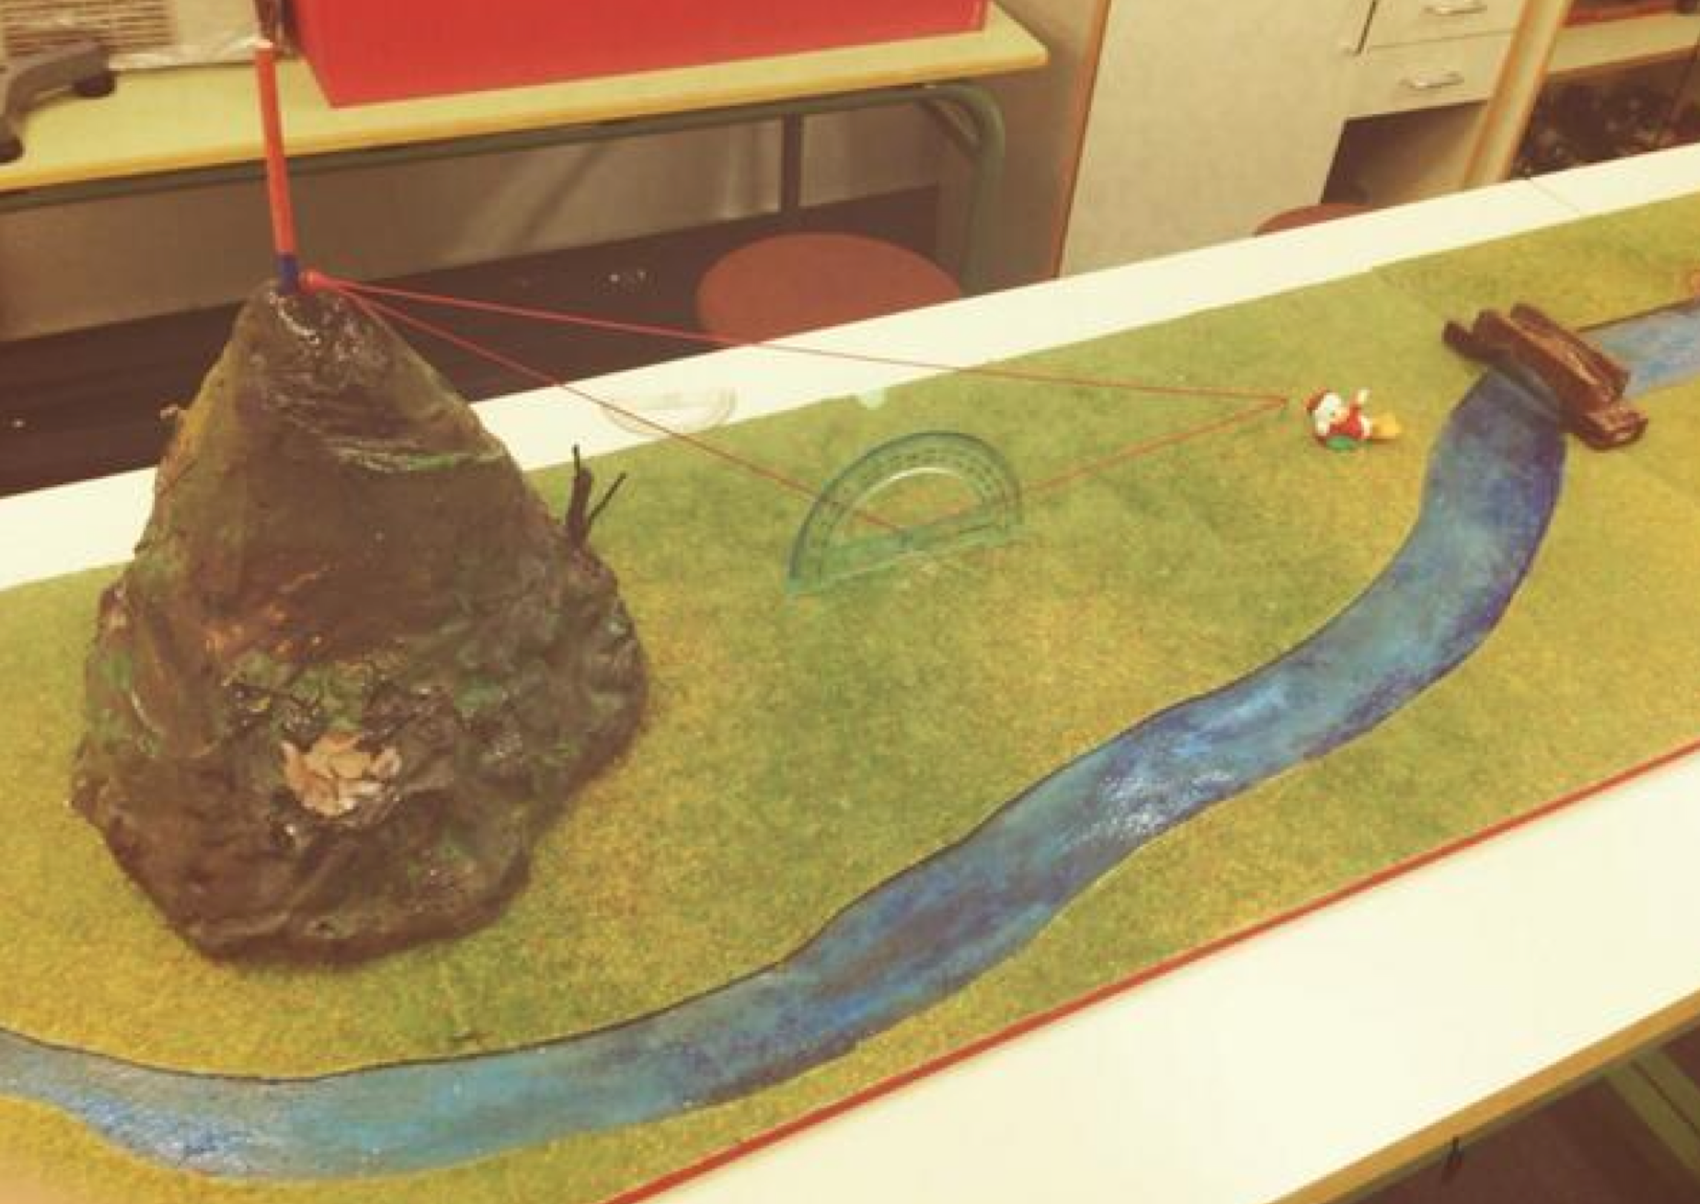
\includegraphics[width=.4\textwidth]{img-triang/triang04.png}
\end{figure}
\end{multicols}

\begin{small}Con unas nociones básicas de trigonometría se puede hacer uso de la misma para calcular alturas y distancias entre puntos en situaciones muy diversas. Presentamos aquí seis usos de la trigonometría para el cálculo de alturas y distancias. Son aplicaciones prácticas en las que se supone que contamos con el material necesario para medir ciertos ángulos (ángulos verticales, sobre todo de elevación, y ángulos horizontales) como, por ejemplo, un teodolito. \footnote{ \textcolor{NavyBlue}{ $\ $ https://lasmatematicas.eu/8-usos-de-la-trigonometria-para-el-calculo-de-alturas-y-distancias/}}\end{small}


%***************************************
\vspace{5mm}

\begin{large}
\textbf{Distancia entre un punto accesible y otro inaccesible}	
\end{large}

\begin{figure}[H]
	\centering
	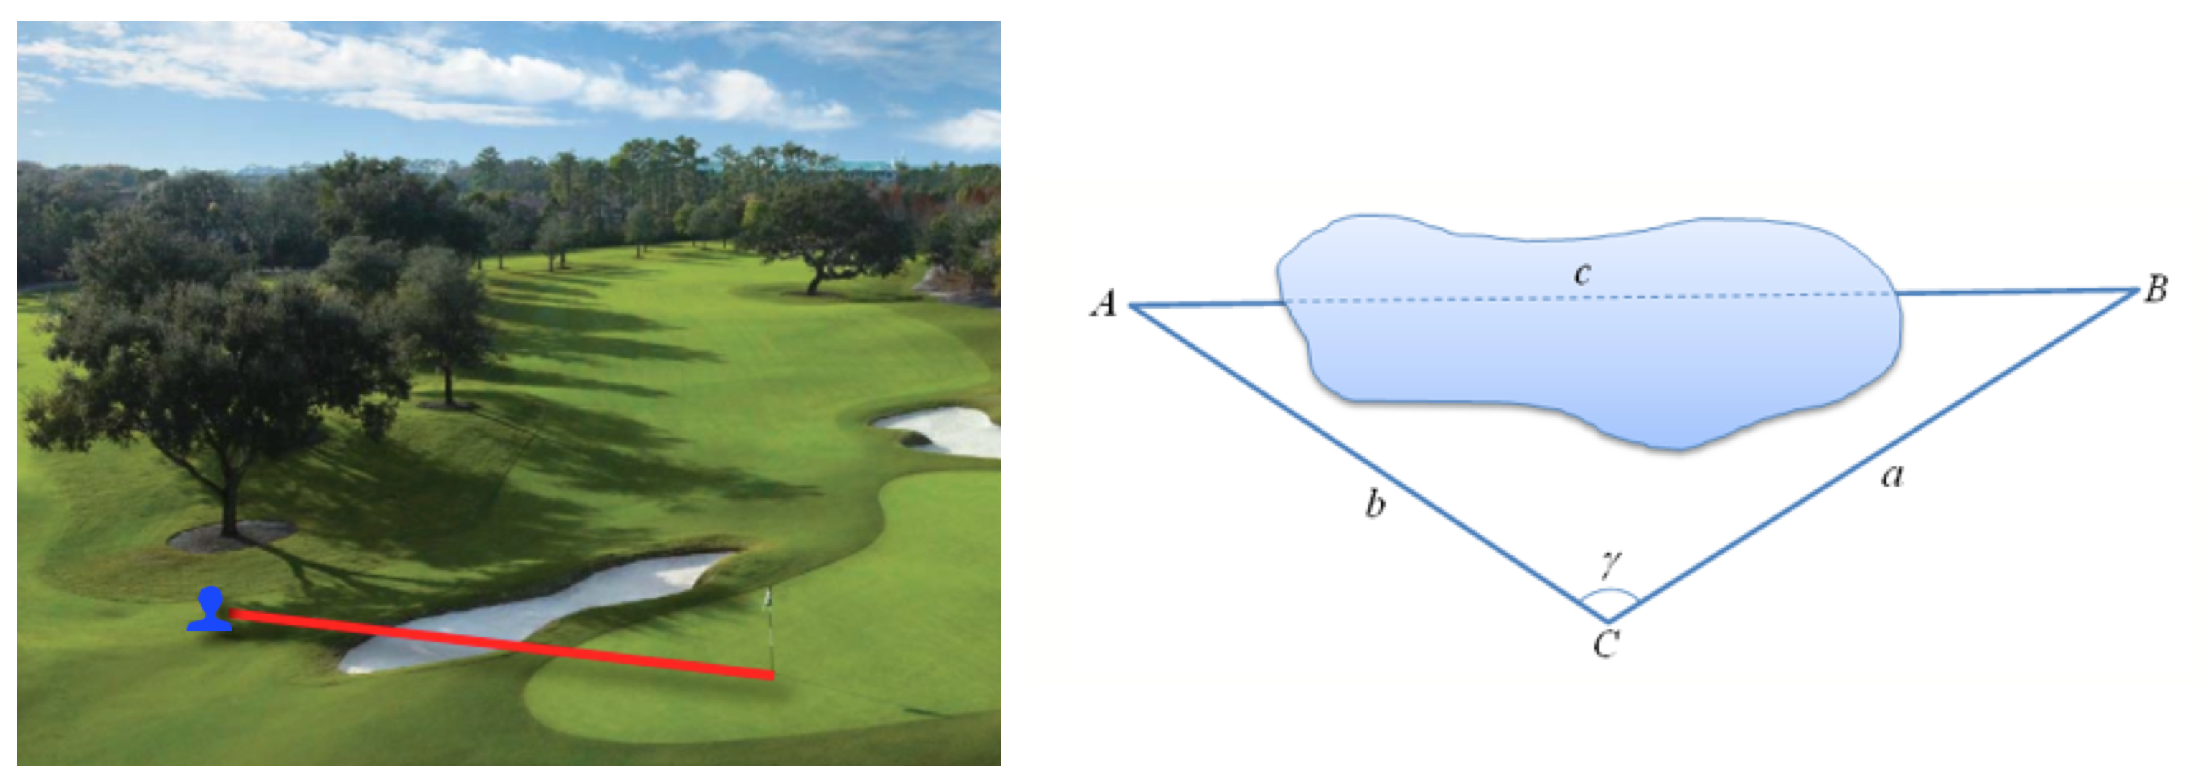
\includegraphics[width=.9\textwidth]{img-triang/topog01.png}
\end{figure}


Se desea medir la distancia $\boldsymbol c$, desde $A$ hasta $B$ pero entre ellos media un obstáculo.

Para efectuar la medida nos situamos en $C$ un punto no alineado con $\overline{AB}$ desde donde podemos medir la distancia a 
$A$ y a $B$, que llamaremos $a$ y $b$, respectivamente. Medimos también el ángulo $C=\widehat{ACB}$.

Con todo ello y aplicando el teorema de cosenos:
$\qquad c^2\ = \ a^2 \ + \ b^2\ - 2\, a\, b\, \cos C$


%**********************************
\vspace{8mm}
\begin{large}
\textbf{Distancia entre dos puntos accesibles entre los que media un obstáculo}	
\end{large}

\begin{figure}[H]
	\centering
	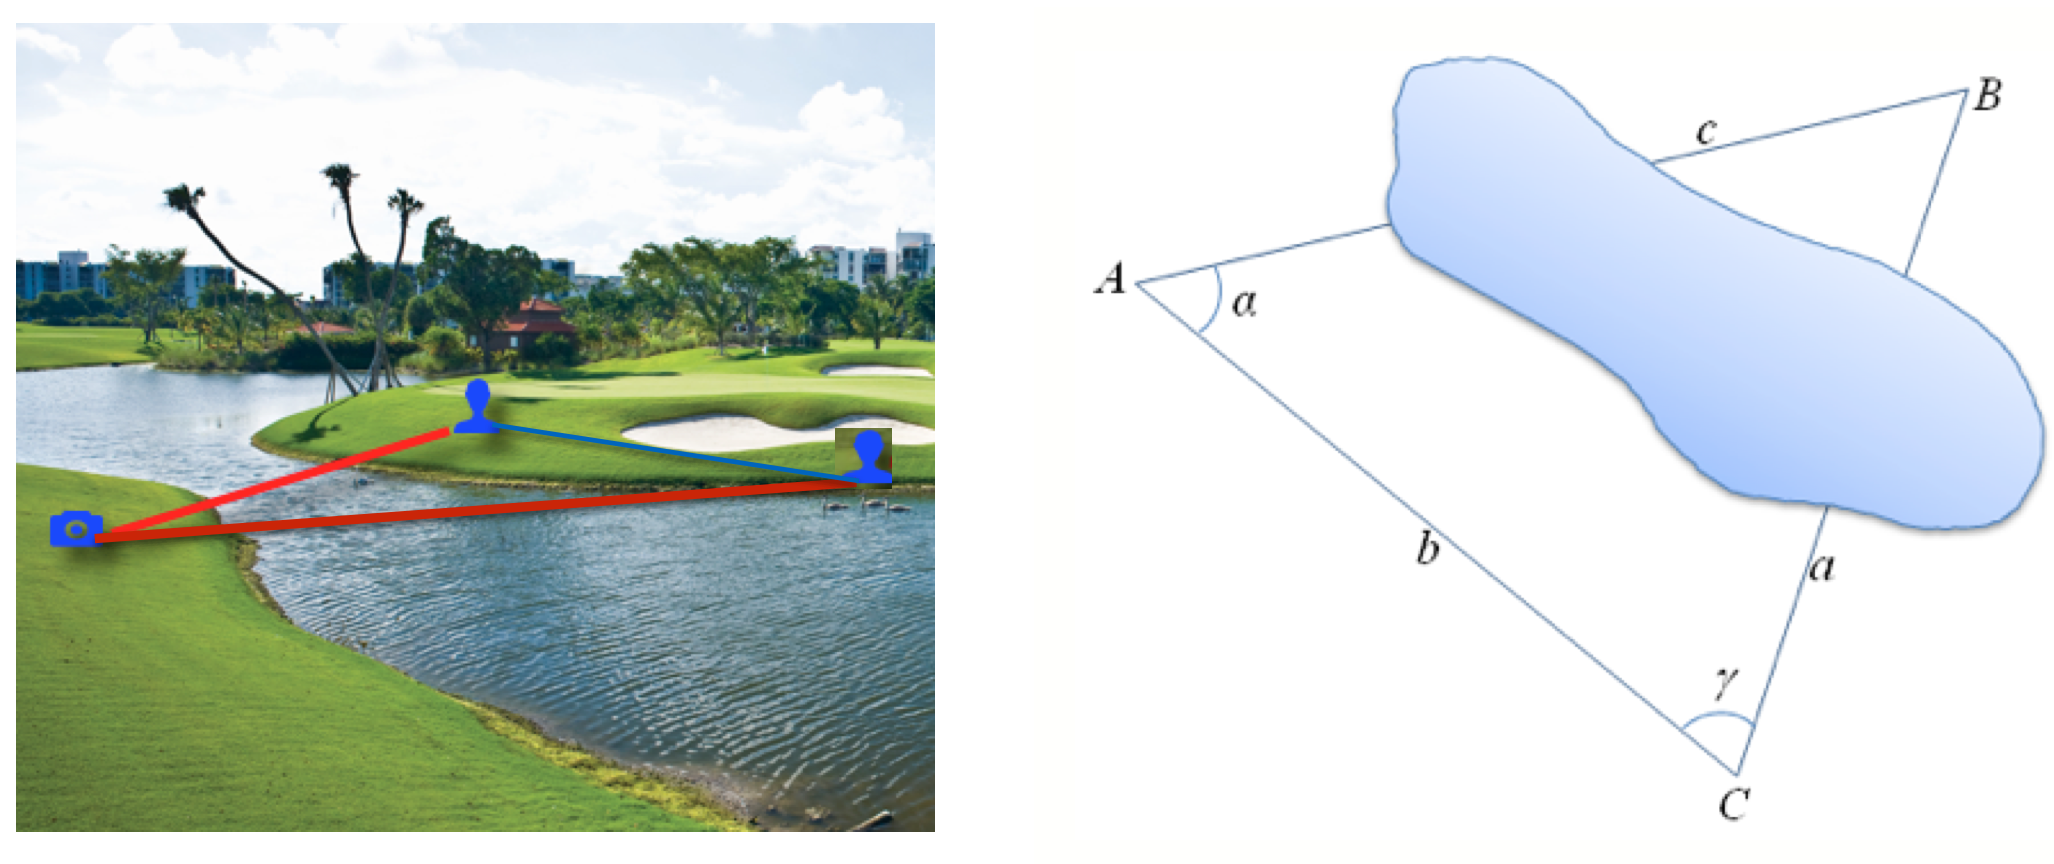
\includegraphics[width=.9\textwidth]{img-triang/topog02.png}
\end{figure}	


Se desea conocer la distancia $\boldsymbol c$ entre $A$ y $B$ entre los que existe un obstáculo pero, a diferencia del caso anterior, no podemos acceder a él.

Elegimos un punto $N$ no alineado con los anteriores al que sí podemos acceder y medimos la distancia hasta $A$, que llamamos $b$. Medimos los ángulos $C=\widehat{ACB}=\gamma$ y $A=\widehat{BAC}=\alpha$.

La medida del tercer ángulo, $B=\widehat{ABC}=\beta$ será la necesaria para que los tres sumen 180$^o$.

Por el teorema de senos, $\qquad \dfrac{b}{\sin B}=\dfrac{c}{\sin C} \ \to \ c=\dfrac{b\sin C}{\sin B}$


%**********************************
\vspace{8mm}
\begin{large}
\textbf{Altura de un punto de pie inaccesible}	
\end{large}

\begin{figure}[H]
	\centering
	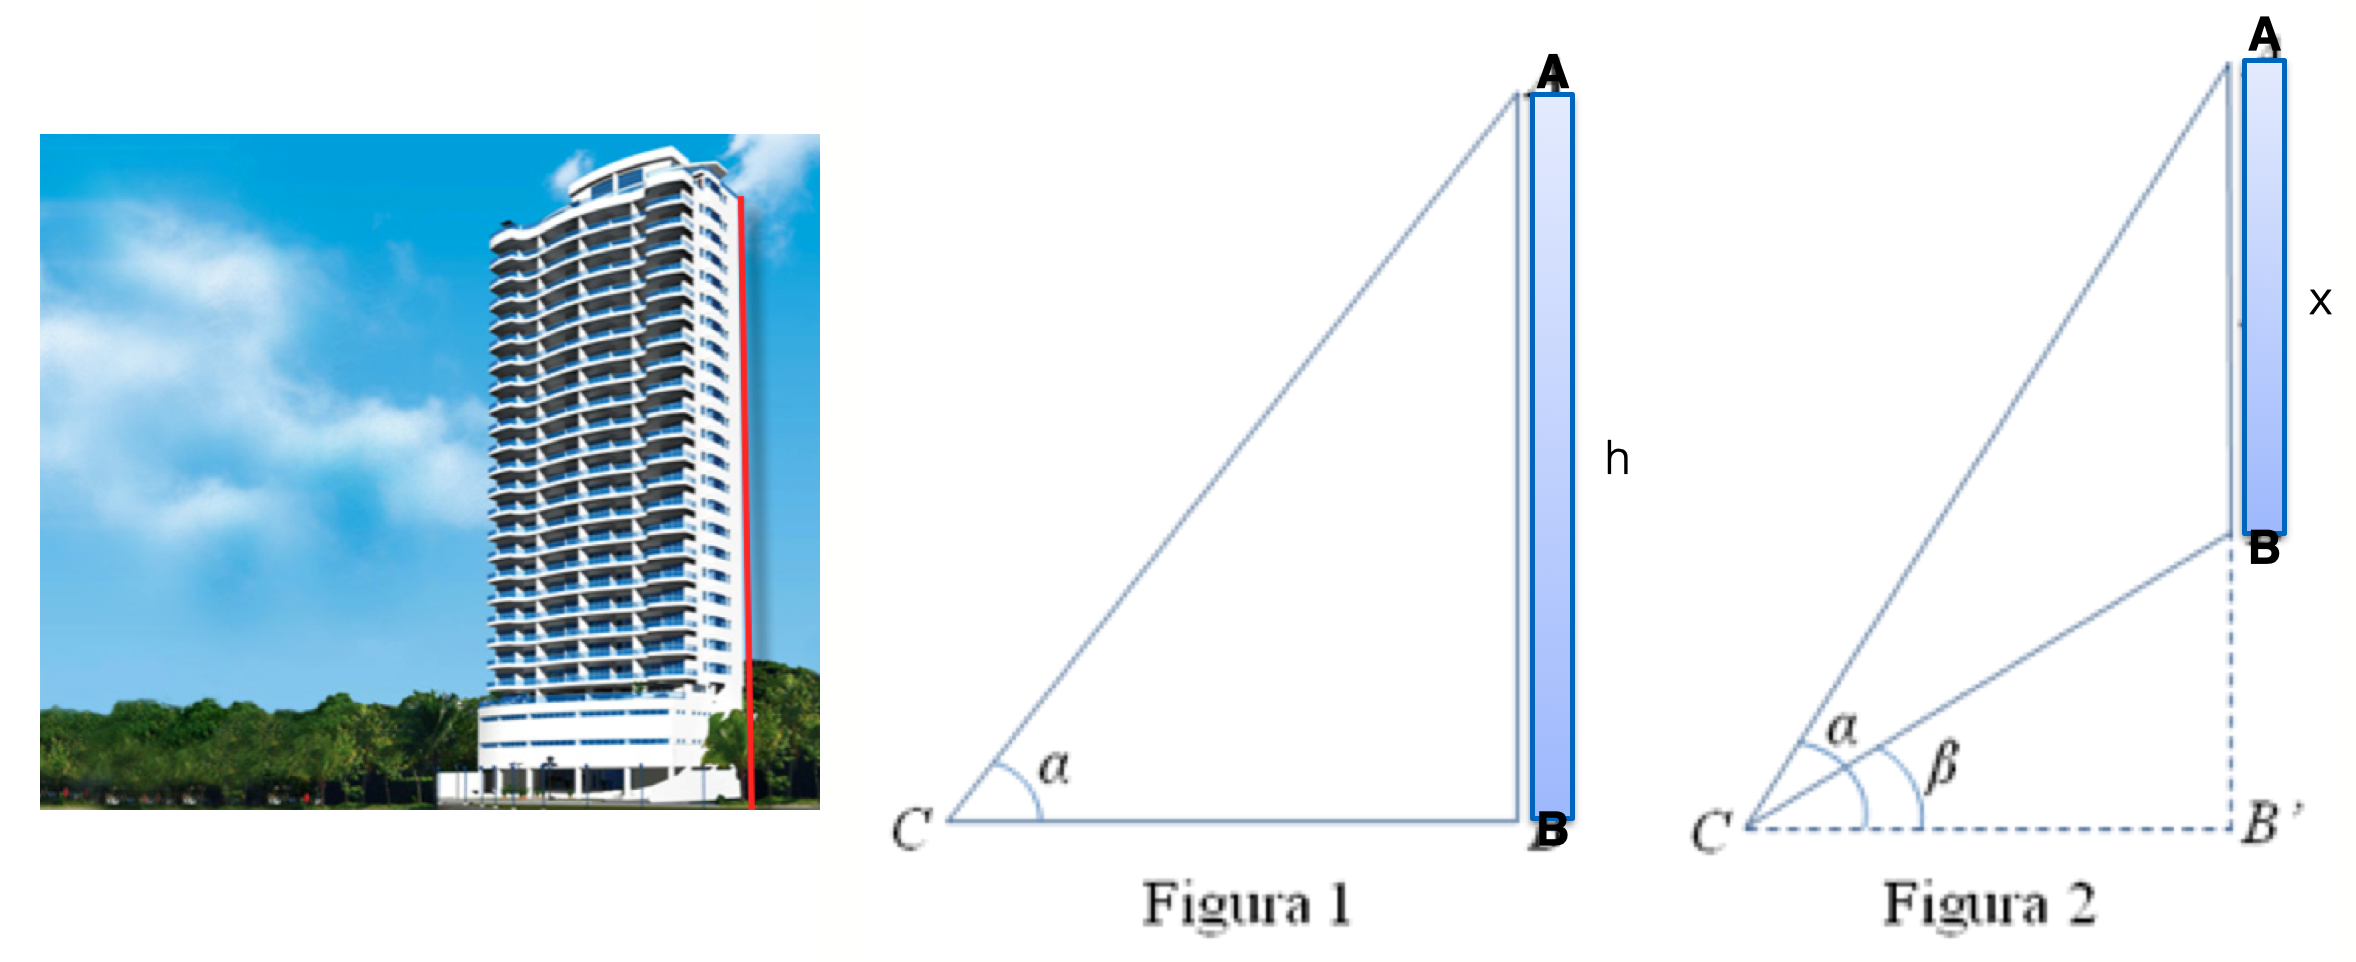
\includegraphics[width=.9\textwidth]{img-triang/topog03.png}
\end{figure}


Podemos tener dos casos: que el suelo sea horizontal (figura 1) o que esté inclinado (figura 2).

\vspace{4mm} $\boldsymbol{\triangleright}\quad$ \textbf{Suelo horizontal} (figura 1):

El triángulo $ABC$ es rectángulo $\quad \Rightarrow \quad \tan \alpha=\dfrac{h}{\overline{CB}} \quad \to \quad h=\overline{CB} \cdot \tan \alpha$



\vspace{4mm}  $\boldsymbol{\triangleright}\quad$ \textbf{Suelo inclinado} (figura 2):

La inclinación del suelo viene determinada por el ángulo $\alpha$ y medimos el ángulo $\alpha=\widehat{ACB'}$, de ahí,

--- el ángulo $\widehat{ACB}=\alpha-\beta$ y el ángulo $\widehat {CAB}=90^o-\alpha\, . \ $ Aplicando el teorema de senos:

 $\dfrac{\overline{CB}}{\sin \widehat {CAB}}=\dfrac{x}{\sin \widehat{ACB}}  \quad \to \quad \dfrac{\overline{CB}}{\sin (90-\alpha)}=\dfrac{x}{\sin (\alpha-\beta)} \quad \Rightarrow \quad  x=\dfrac{\overline{CD} \cdot \sin (\alpha-\beta)}{\sin (90-\alpha)}$

%**********************************
\vspace{8mm}
\begin{large}
\textbf{Altura de un punto de pie inaccesible desde un terreno horizontal sin obstáculos}	
\end{large}

\begin{figure}[H]
	\centering
	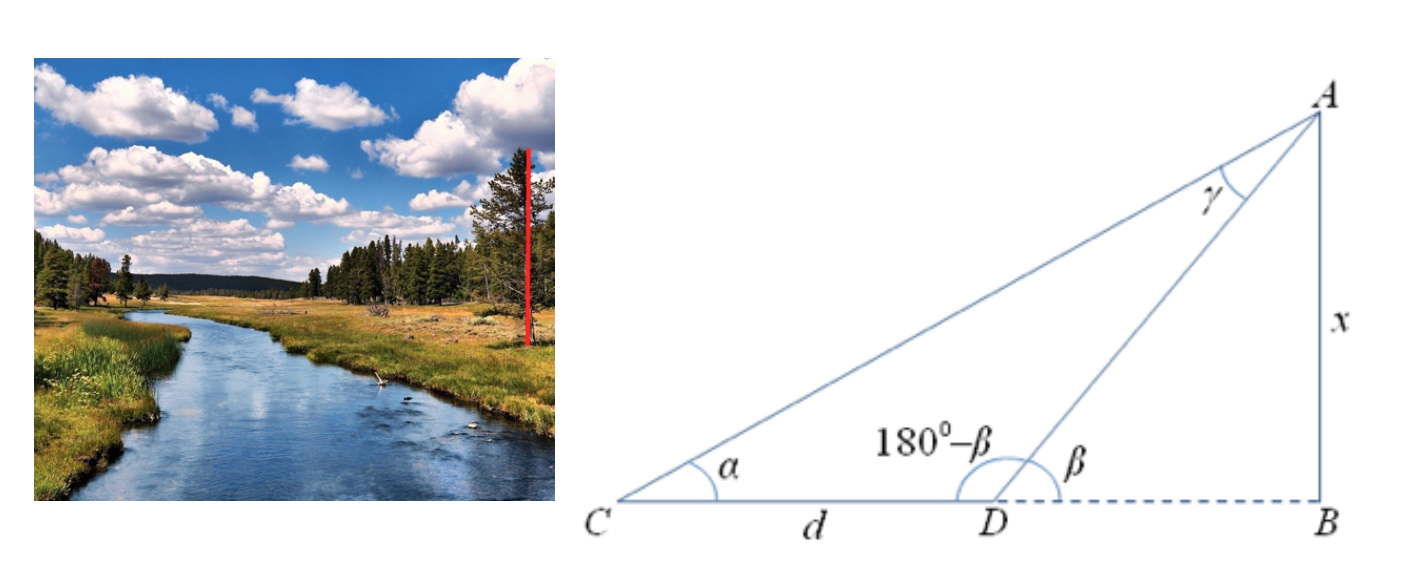
\includegraphics[width=.9\textwidth]{img-triang/topog04.png}
\end{figure}

Deseamos calcular la altura $x=\overline{AB}$ de un objeto cuyo pie $B$ nos es inaccesible.

Para ello nos situamos en un punto $C$ desde donde observamos $A$ bajo un ángulo $\widehat{ACB}=\alpha$. Desde $C$ avanzamos en dirección $\overline{CB}$ hasta el punto $D,\ \overline{CD}=d$ desde donde observamos $A$ bajo un ángulo $\widehat{ABD}=\beta$.

La estrategia a seguir es calcular $\overline{AC}$ en el triángulo $ACD$ y luego calcular $x$ en el triángulo rectángulo $ACB$ \textcolor{gris}{(también se podría calcular $\overline{AD}$ en el triángulo $ACD$ y luego calcular $x$ en el triángulo rectángulo $ADB$)}

En el triángulo $ACD$, son conocidos $C=\alpha$ y $D=180^o-\beta$, por lo que el ángulo $A=\gamma=180-\alpha-(180-\beta)=\beta-\alpha$

Teorema de senos en $ACD:\qquad \dfrac{\overline{AC}}{\sin(180-\beta)}=\dfrac{d}{\sin \gamma} \quad \to \quad \overline{AC}=\dfrac{d\sin(180-\beta)}{\sin \gamma}$

Definición de seno en $ACB:\qquad \sin \alpha=\dfrac{x}{\overline{AC}} \quad \Rightarrow \quad x=\overline{AC} \cdot \sin \alpha$

\textcolor{gris}{Si interesa la distancia del primer punto de observación, $C$, al pie del objeto, $B$, haríamos: $\ \cos \alpha=\dfrac{\overline{CB}}{\overline{AC}} \quad \to \quad \overline{CB}=\overline{AC} \cdot \cos \alpha$}

\vspace{8mm}
\begin{large}
\textbf{Altura de un objeto situado sobre un montículo situado en un terreno horizontal sin obstáculos}	
\end{large}

\begin{figure}[H]
	\centering
	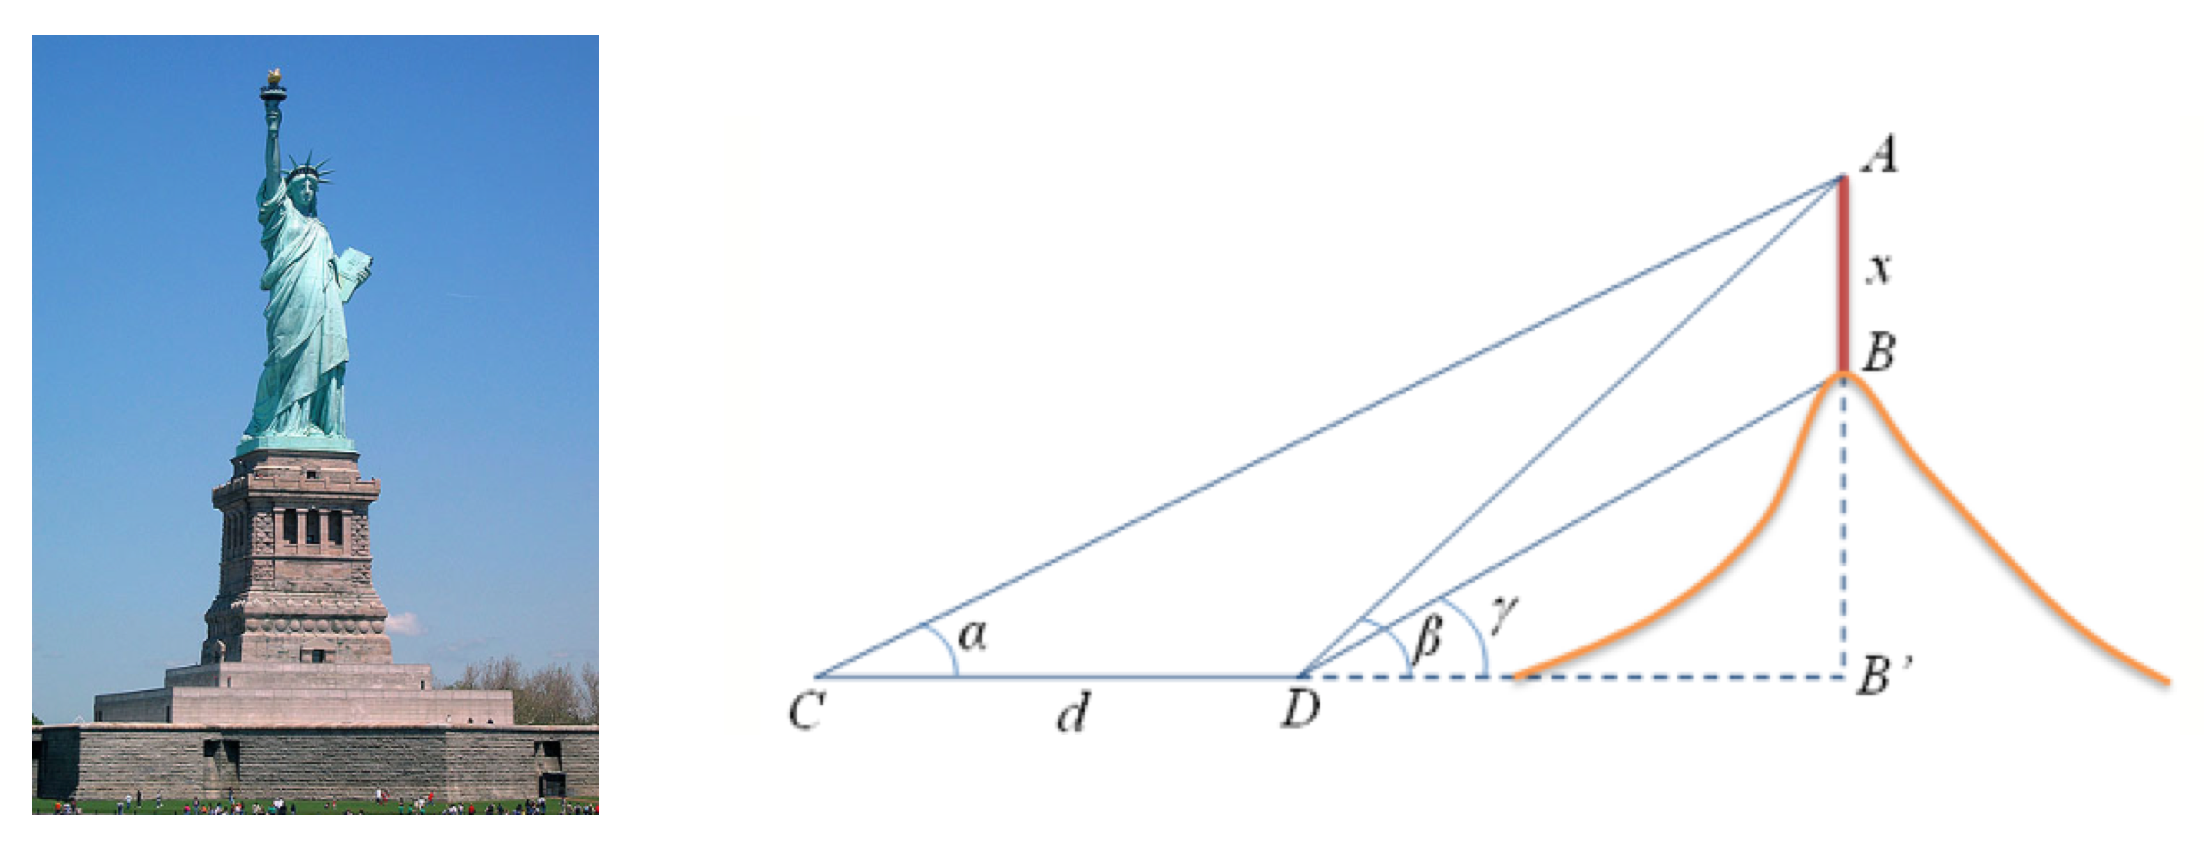
\includegraphics[width=.9\textwidth]{img-triang/topog05.png}
\end{figure}

Deseamos conocer la altura $x=\overline{AB}$.

Nos situamos en un punto arbitrario del terreno $C$ desde donde medimos el ángulo de elevación que llamaremos $\alpha$. 

Nos desplazamos a otro punto $D$, más cercano al objeto y en dirección a él \textcolor{gris}{($\overline{CB'}$)}. Desde allí medimos $\overline{CD}=d$ y los ángulos de elevación de $A$ y $B$ que llamaremos $\beta$ y $\gamma$, respectivamente.

Del triángulo $ACD$ conocemos un lado, $\overline{CD}=d$ y dos ángulos, $\widehat{ACD}=\alpha$ y $\widehat{ADC}=180-\beta$, por lo que el tercer ángulo será $\ \widehat{CAD}=180-\alpha-(180-\beta)=\beta-\alpha$

Por teorema de senos en $ACD:\qquad \dfrac{\overline{AD}}{\sin \widehat{ACD}}=\dfrac{d}{\sin \widehat{ CAD}} \quad \to \ \overline{AD}=\dfrac{d\, \sin \alpha}{\sin (\beta-\alpha)}$

Ahora, en el triángulo $ABD$ conocemos un lado, $\overline{AD}$ y dos ángulos, $\widehat{ADB}=\beta-\gamma$ y  $\widehat{DAB}=90-\beta$. De nuevo, con el ángulo que falta se completarán 180$^o$: $\ \ \widehat{ABD}=180-(\beta-\gamma)-(90-\beta)=90+\gamma$

Por teorema de senos en $ADB:\qquad  \dfrac{x}{\sin \widehat{ADB}}=\dfrac{\overline{AD}}{\sin \widehat{ABD}} \quad \Rightarrow \quad x=\dfrac{\overline{AD} \, \sin(\beta-\gamma)}{\sin (90+\gamma)}$

%%%%%%%
\vspace{8mm}
\begin{large}
\textbf{Altura de un punto de pie inaccesible desde un terreno inclinado y sin obstáculos}	
\end{large}

\begin{figure}[H]
	\centering
	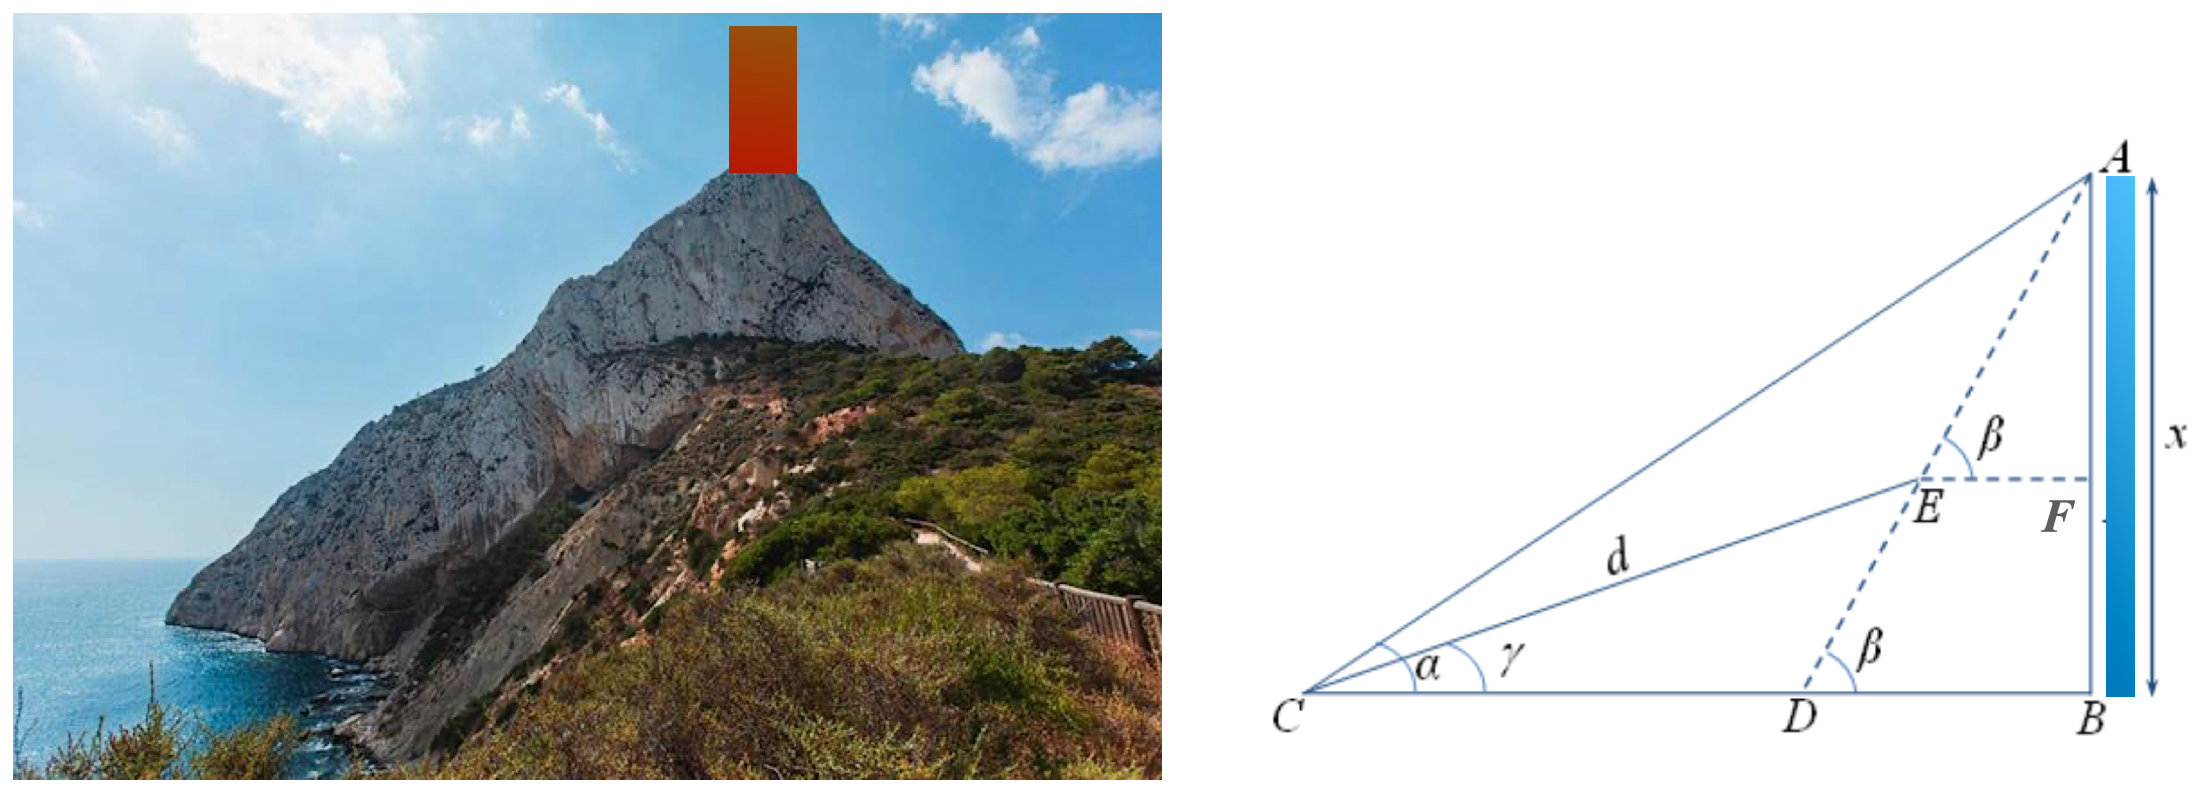
\includegraphics[width=.9\textwidth]{img-triang/topog07.png}
\end{figure}

Deseamos calcular la altura $\overline{AB}=x$ a la que está de un objeto de pie inaccesible situado sobre un terreno horizontal sin obstáculos.

Llamamos $\gamma$ a la inclinación del terreno. Pretendemos calcular $\overline{AC}$ del triángulo $ACE$, para luego, a través del triángulo $ABC$ del que es su hipotenusa, calcular $x$.

Desde un punto alejado $C$ calculamos el ángulo de elevación de $A$, $\ \widehat{BCA}=\alpha$. Medimos la distancia $d=\overline{CE}$ sobre el plano inclinado y desde alli, desde $E$ volvemos a medir el ángulo de elevación de $A$, $\widehat{FEA}=\beta$.

 $\widehat{ACE}=\alpha-\gamma;\quad \widehat{CAE}=\widehat{CAB}-\widehat{DAB}=(90-\alpha)-(90-\beta)=\beta-\alpha$
 
 Con ello, $\ \widehat{CEA}=180-\widehat{ACE}-\widehat{CAE}=180-(\alpha-\gamma)-(\beta-\alpha)=180+\gamma-\beta$
 
 Teorema de senos al triángulo $ACE:\quad \dfrac{\overline{AC}}{\sin \widehat{CEA}}=\dfrac{d}{\sin \widehat{CAE}} \ \ \to \ \ \overline{AC}=\dfrac{d\cdot \sin(180+\gamma-\beta)}{\sin(\beta-\alpha)}$
 
 Definición de seno en $ABC:\quad \sin \alpha=\dfrac{x}{\overline{AC}} \quad \to \quad x=\overline{AC}\cdot \sin \alpha$

%%%%%%%%%
\vspace{8mm}
\begin{large}
\textbf{Distancia entre dos puntos ambos inaccesibles}	
\end{large}

\begin{figure}[H]
	\centering
	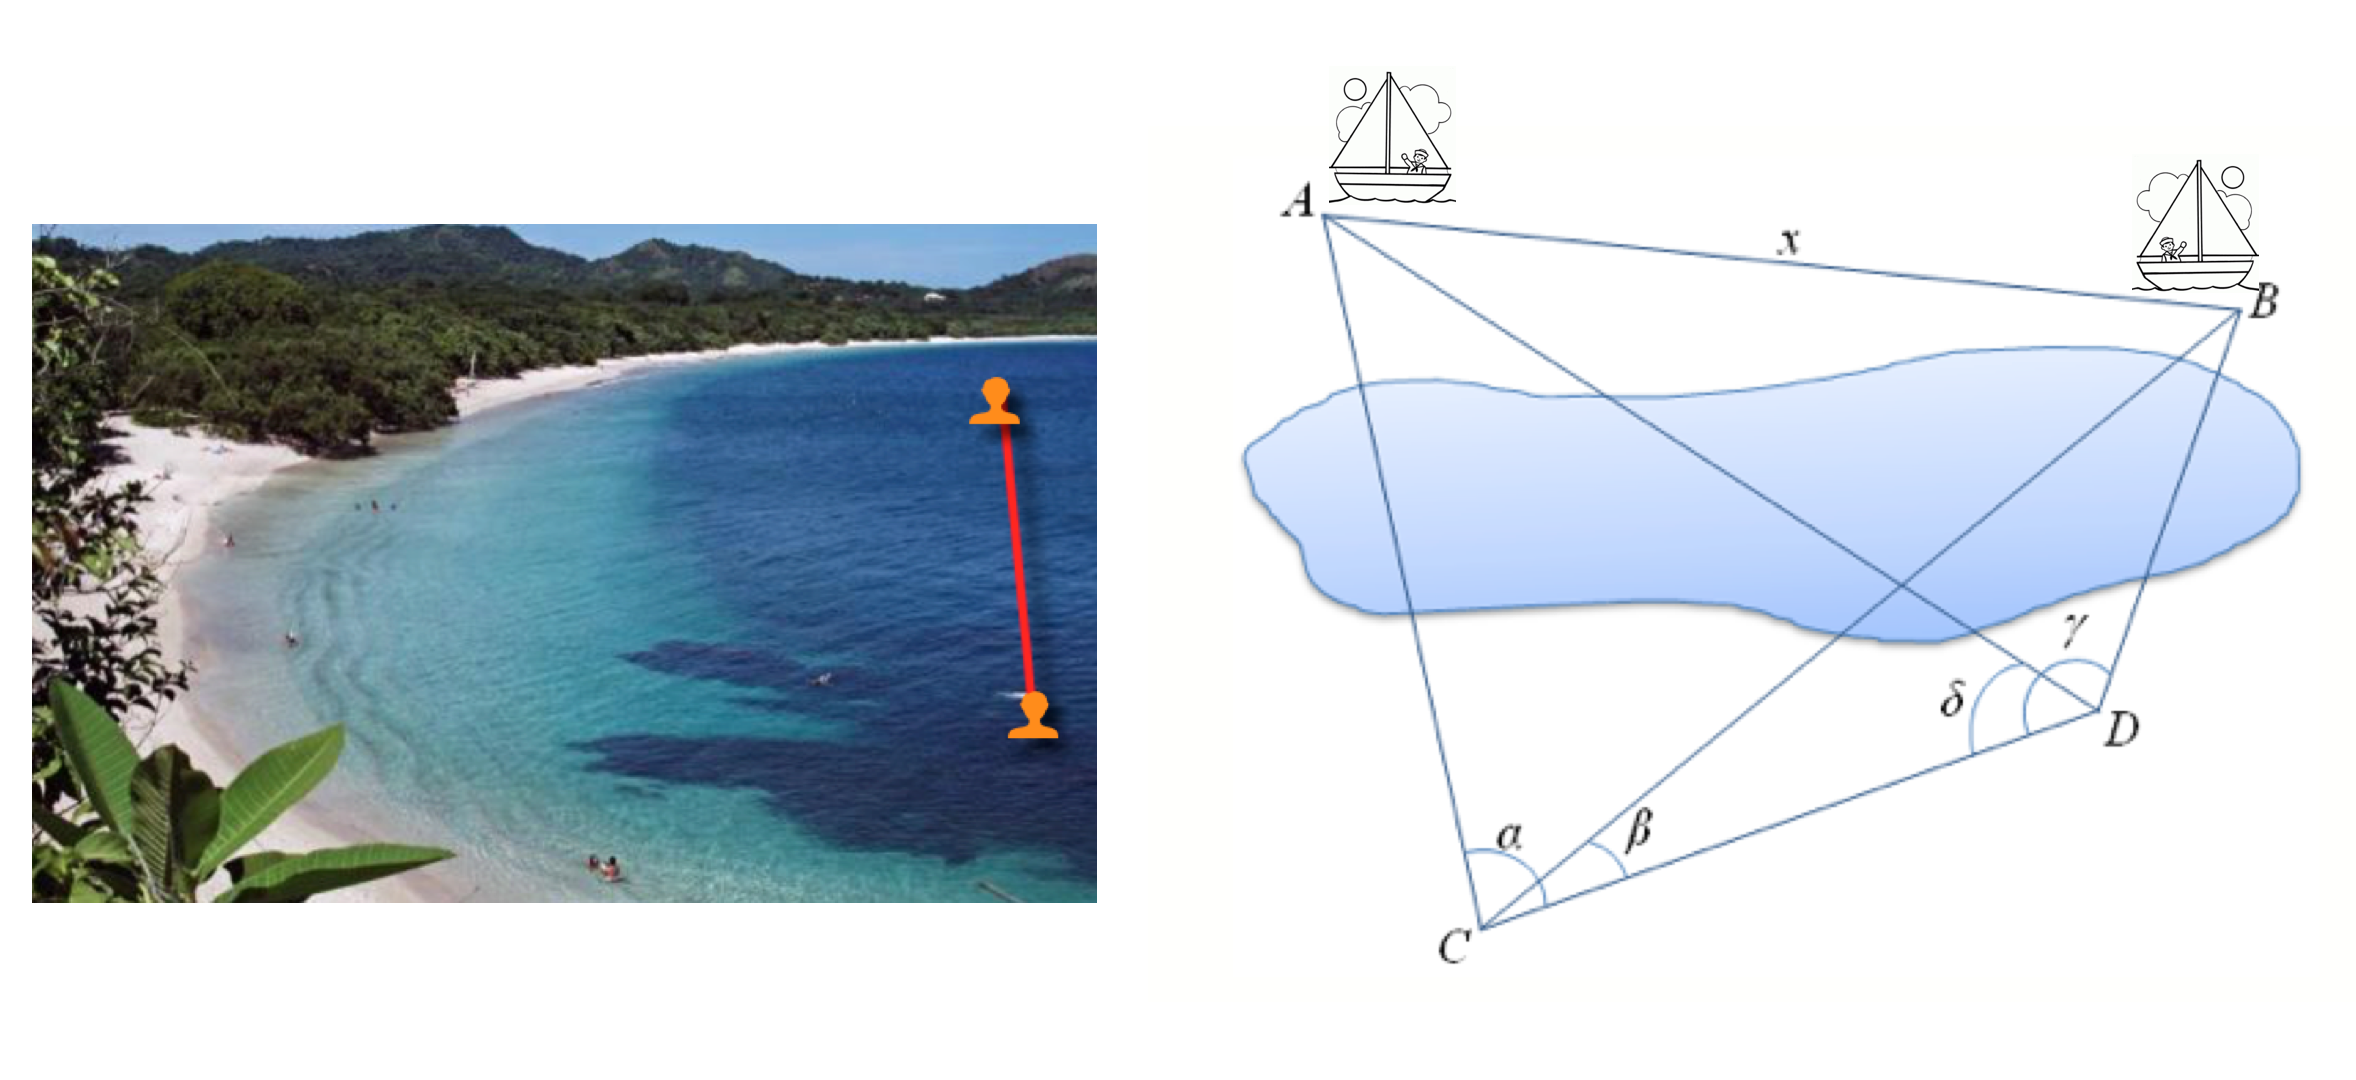
\includegraphics[width=.9\textwidth]{img-triang/topog06.png}
\end{figure}

Deseamos medir la distancia $x=\overline{AB}$ entre dos puntos que nos son inaccesibles (los barcos en la figura). Para elle medimos una base arbitraria $\overline{CD}$ (en la costa).

Desde $C$ medimos los ángulos $\widehat{ACD}=\alpha$ y $\widehat{BCD}=\beta$. Desde $D$ hacemos lo mismo, $\widehat{CDB}=\gamma$ y $\widehat{CDA}=\delta$. Con estas medidas podemos determinar los ángulo $\widehat{CAD}=180-\alpha-\delta$ y $\widehat{CBD}=180-\beta-\gamma$.

El algoritmo consta de tres partes: 

\vspace{-2mm} \begin{itemize}
\vspace{-2mm} \item determinar $\overline{AC}$ en el triángulo $ACD$ por teorema de senos.
\vspace{-2mm} \item determinar $\overline{BC}$ en el triángulo $BCD$ por teorema de senos.
\vspace{-2mm} \item determinar $x=\overline{AB}$ en el triángulo $ACB$ por teorema de cosenos.
\end{itemize}

 $\triangleright \ \ $ Triángulo $ACD:\qquad \dfrac{\overline{AC}}{\sin \widehat{CDA}}=\dfrac{\overline{CD}}{\sin \widehat{CAD}} \quad \to \quad \overline{AC}=\dfrac{\overline{CD}\,\sin \delta}{\sin (180-\alpha-\delta)}$

 $\triangleright \ \ $ Triángulo $BCD:\qquad \dfrac{\overline{BC}}{\sin \widehat{BDC}}=\dfrac{\overline{CD}}{\sin \widehat{CBD}} \quad \to \quad \overline{BC}=\dfrac{\overline{CD}\, \sin \gamma}{\sin (180-\beta-\gamma)}$
 
 $\triangleright \ \ $ Triángulo $ABC:\qquad x^2\ =\ \overline{AC}^2+\overline{BC}^2-2\, \overline{AC} \cdot \overline{BC} \, \cos(\alpha-\beta)$



\vspace{1cm}


\begin{myexampleblock}{El teodolito}

\vspace{2mm} El teodolito es un instrumento de medición mecánico-óptico que se utiliza para obtener ángulos verticales y horizontales con  una precisión elevada. Es portátil y manual; está hecho con fines topográficos e ingenieriles, sobre todo para las triangulaciones. Con ayuda de una mira y mediante la taquimetría, puede medir distancias. Un equipo más moderno y sofisticado es el teodolito electrónico.

\vspace{2mm} Básicamente, el teodolito es un telescopio montado sobre un trípode y con dos círculos graduados, uno vertical y otro horizontal, con los que se miden los ángulos con ayuda de lentes.

\vspace{2mm} El teodolito también es una herramienta muy sencilla de transportar. Por eso es una herramienta que tiene muchas garantías y ventajas en su utilización. Es su precisión en el campo lo que lo hace importante y necesario para la construcción.

\begin{multicols}{2}
\begin{figure}[H]
	\centering
	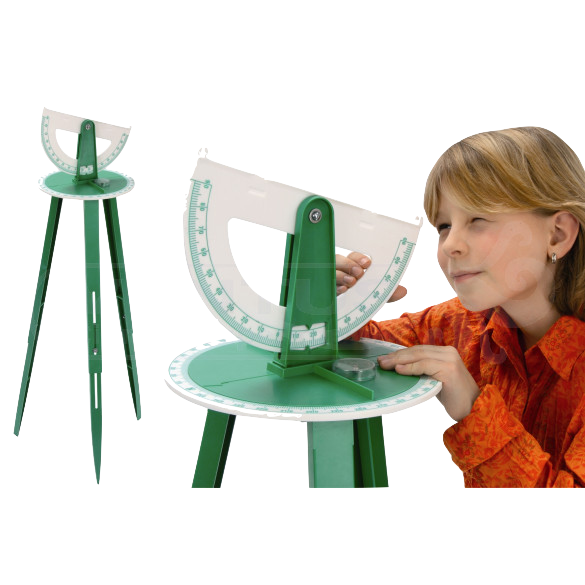
\includegraphics[width=.4\textwidth]{img-triang/teodolito.png}
\end{figure}
\begin{figure}[H]
	\centering
	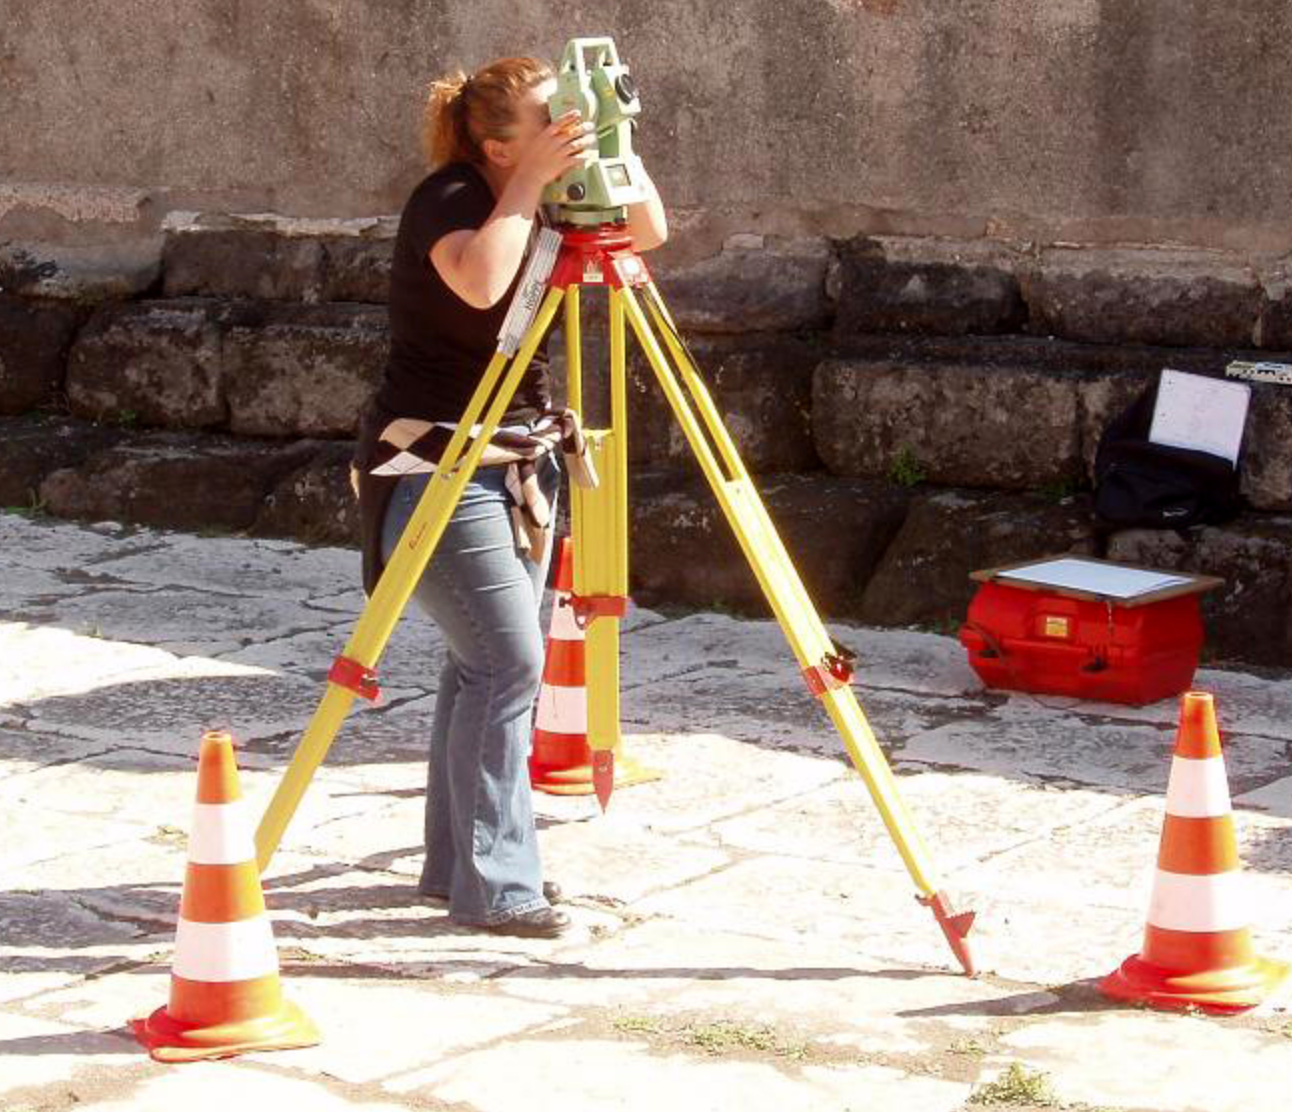
\includegraphics[width=.4\textwidth]{img-triang/teodolitop.png}
\end{figure}
\end{multicols}
	
\end{myexampleblock}

%%%%%%%%%%%%%%%%%%%%%%%


\vspace{0.3cm}
\section{Ejercicios}

\begin{tikzpicture}
	\fill [left color=red!50, right color=teal!50] (0,0) rectangle (3.5,.1);
	\fill [left color=teal!50, right color=blue!50] (3.5,0) rectangle (7.5,.1);
	\end{tikzpicture}
\vspace{0.3cm}





%%%%
\begin{miejercicio}[ Aplicaciones topográficas 1/7]


\begin{multicols}{2}
Un túnel $\overline{AB}$ ha de atravesar una montaña. Para calcular su longitud , desde un punto no alineado con $A$ y $B$ se toman las siguientes medidas:

$\quad \overline{AC}=1250\, \mathrm{m};\ \ \overline{BC}=1700\, \mathrm{m};$

$\quad \widehat{ACB}=C=132^o$
	\begin{figure}[H]
	\centering
	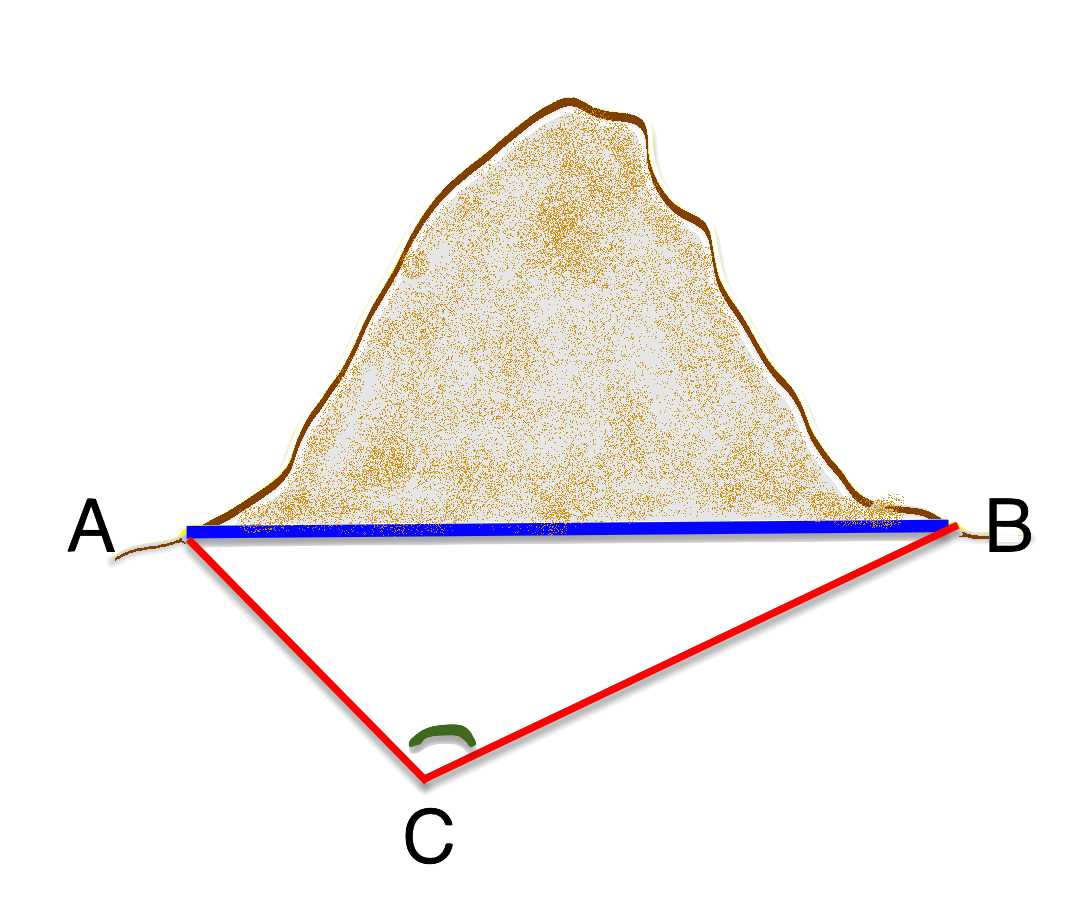
\includegraphics[width=.3\textwidth]{img-triang/triang15.png}
\end{figure}
\end{multicols}

\vspace{-10mm}
\rule{250pt}{0.1pt}

\vspace{2mm} Tenemos $\ b=1250,\ a=1700, \ C=132^o \ \to \ $ por teorema de cosenos,

\vspace{2mm} $c=\sqrt{1250^2+1700^2-2\cdot 1250\cdot 1700\cdot \cos 132^o}=2701,17 \, \textrm{m}$ será la  longitud del túnel.

	
\end{miejercicio}






%************
\begin{miejercicio}[ Aplicaciones topográficas 2/7]

\begin{multicols}{2}

	Para calcular la anchura $\overline{AB}$ de un río se elige un punto $C$ que está en la misma orilla que y se toman las siguientes medidas: 
	
\vspace{2mm}  $\overline{AC}=67\, \mathrm{m};\ \ \widehat{BAC}=B=99^o;\ \ \widehat{ACB}=C=20^o$
 
\vspace{2mm}  ?`Cuál es la anchura del río?
 
	\begin{figure}[H]
	\centering
	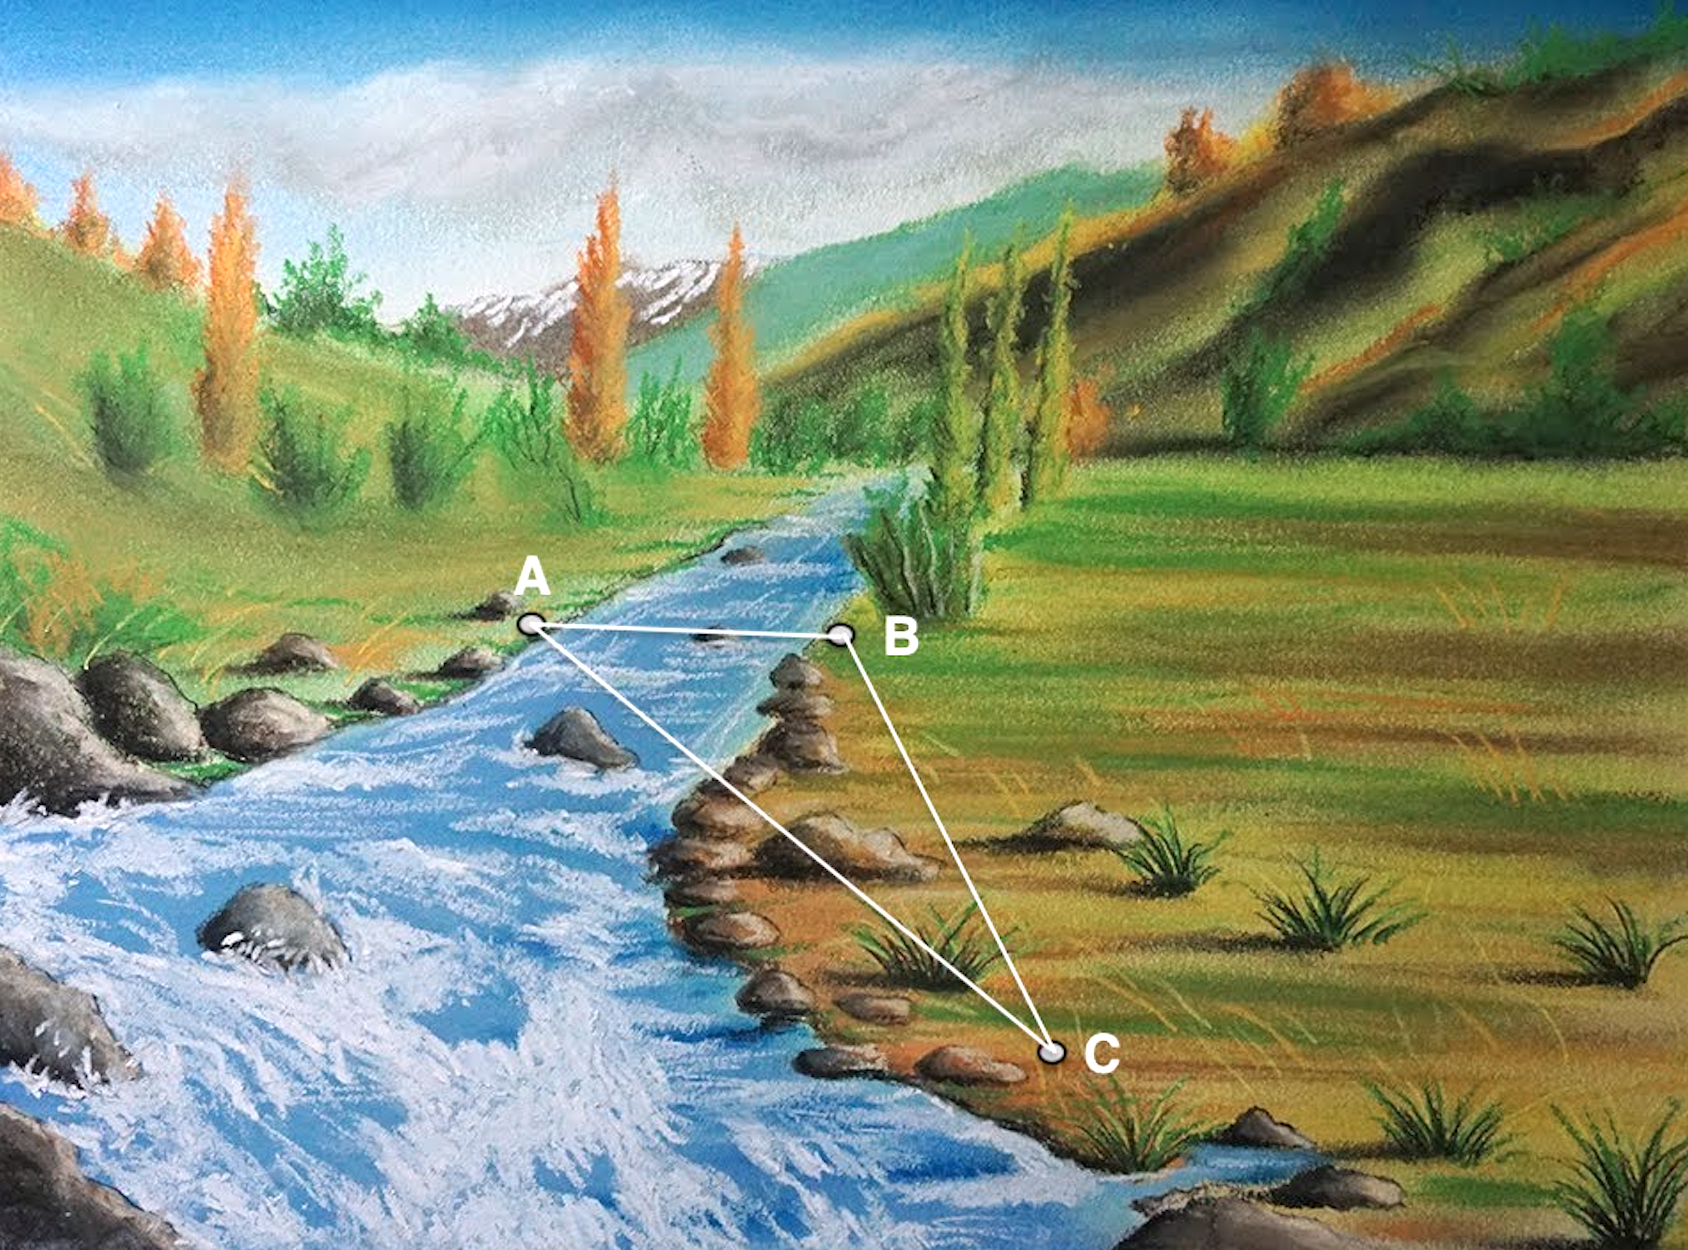
\includegraphics[width=.4\textwidth]{img-triang/triang16.png}
\end{figure}
\end{multicols}

\vspace{-6mm}

\rule{250pt}{0.1pt}

\vspace{2mm} Ahora, $\ b=67,\ C=20^o,\ B=180-(99+20)=61^o,\ $ por teorema de senos,

\vspace{2mm} $\dfrac{b}{\sin B}=\dfrac{c}{\sin C} \ \to \ c=\dfrac{b\, \sin C}{\sin B}=\dfrac{67\cdot \sin 20}{\sin 61}=26.2\, \mathrm{m}$ anchura del río.

	
\end{miejercicio}


%************
\begin{miejercicio}[ Aplicaciones topográficas 3/7]

\begin{multicols}{2}

Un camino plano de $10$ metros de largo y que forma un ángulo de $25^o$ con la horizontal, conduce al pie de una gran torre. Calcular la altura de ésta, sabiendo que desde el inicio del pasillo el ángulo de elevación de su punto más alto es de $82^o$.
 
	\begin{figure}[H]
	\centering
	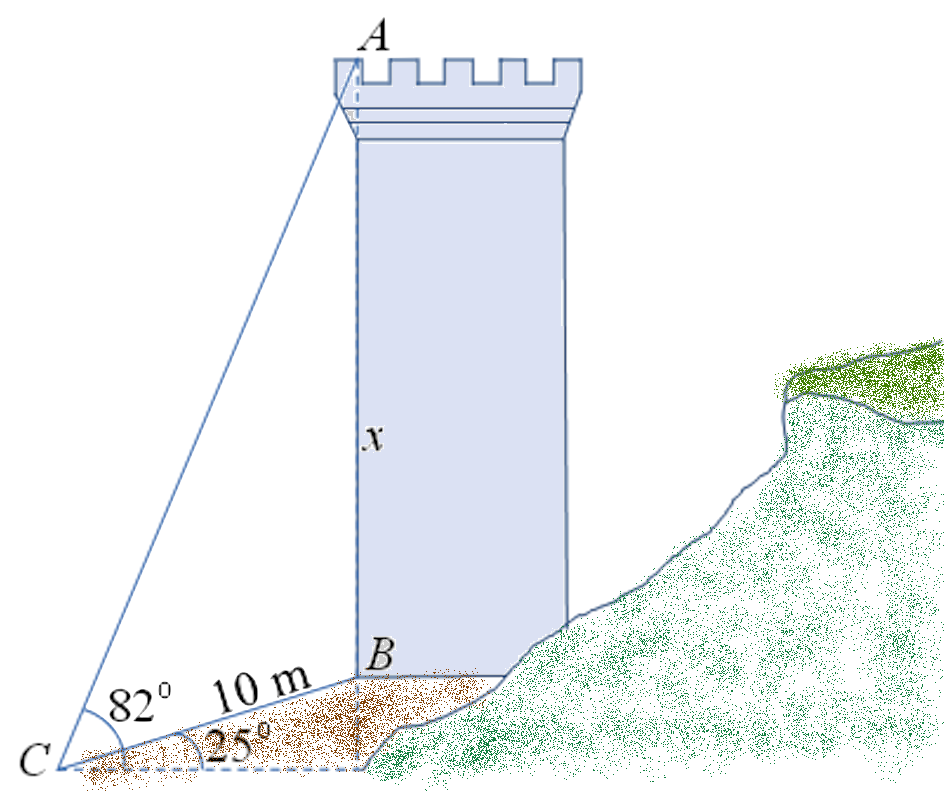
\includegraphics[width=.3\textwidth]{img-triang/triang17.png}
\end{figure}
\end{multicols}

\vspace{-8mm}


\rule{250pt}{0.1pt}

\vspace{2mm} $x=\overline{AB},\ C=\widehat{ACB}=82-25=57^o;\ A=\widehat{CAB}=90-82=8^o;\ \overline{CB}=a=10$, por teorema de senos en ABC:

\vspace{2mm} $\dfrac{x}{\sin C}=\dfrac{a}{\sin A}\ \to \ x=\dfrac{a\, \sin C}{\sin A}=\dfrac{10\, \sin 57}{\sin 8}=60.26 \, \mathrm{m}$ altura de la torre.

	
\end{miejercicio}


%************
\begin{miejercicio}[ Aplicaciones topográficas 4/7]


\begin{multicols}{2}

Desde un punto a ras de suelo se ve la azotea de un edificio con un ángulo de elevación de $48^o$. Avanzando $20$ metros en dirección al edificio, el ángulo de elevación se incrementa en $14^o$. 

Calcular la altura del edificio.
 
	\begin{figure}[H]
	\centering
	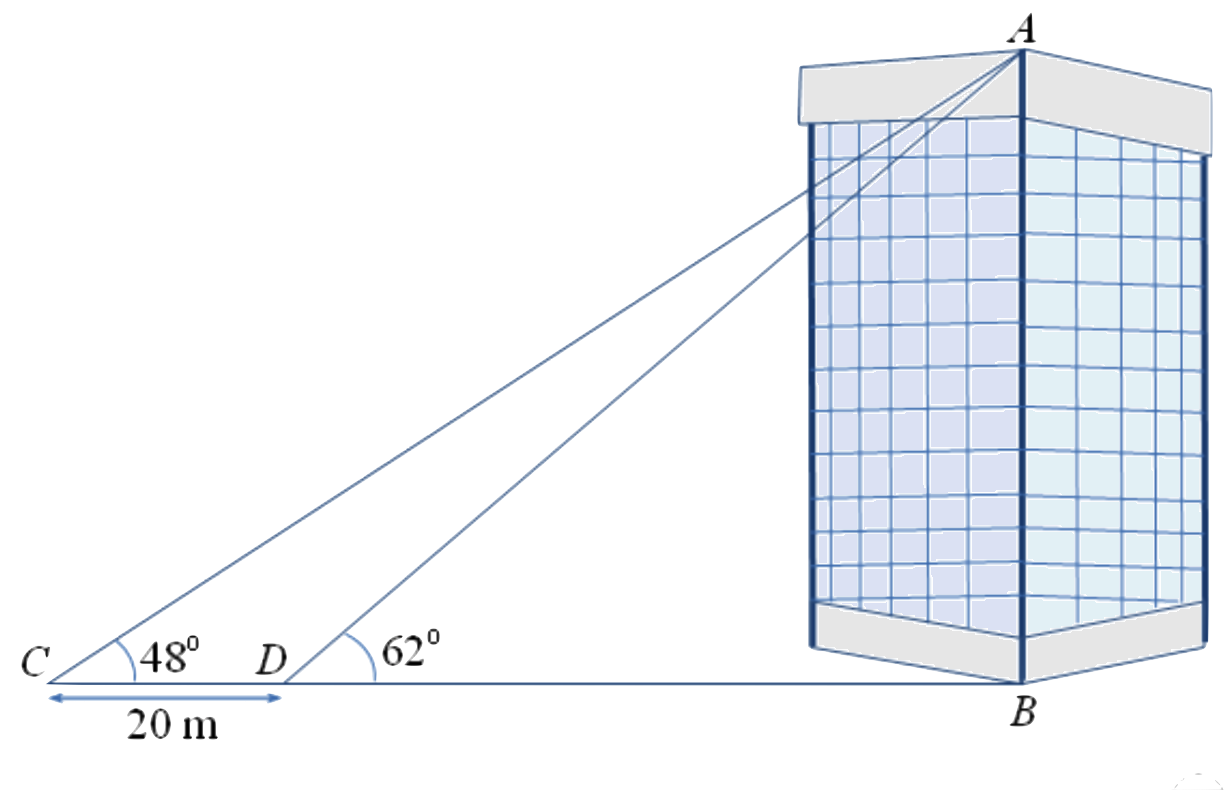
\includegraphics[width=.4\textwidth]{img-triang/triang18.png}
\end{figure}
\end{multicols}

\vspace{-8mm}

\rule{250pt}{0.1pt}

\vspace{2mm} En el triángulo $ABC:\ \ \widehat{CDA}=180-62=118^o;\ \ \widehat{CAD}=180-48-118=14^o;\ \ \overline{CD}=20\, \mathrm{m}\, . \ $ Por teorema de senos,

\vspace{2mm} $\dfrac{\overline{AC}}{\sin \widehat{CDA}}=\dfrac{\overline{CD}}{\sin \widehat{CAD}}\ \to \ \overline{AC}=\dfrac{\overline{CD}\, \sin \widehat{CDA}}{\sin \widehat{CAD}}=\dfrac{20\cdot \sin 118}{\sin 14}=77.99\, \mathrm{m}$

\vspace{2mm} Finalmente, del triángulo $ABC,\quad \sin \widehat{ACB}=\dfrac{ \overline{AB}}{\overline{AC}}\ \to \ \overline{AB}=77.99 \cdot \sin 48=54.26 \, \mathrm{m}$ es la altura del edificio.

\end{miejercicio}


%************
\begin{miejercicio}[ Aplicaciones topográficas 5/7]

\begin{multicols}{2}

El ángulo de elevación de una peña $\overline{AB}$
 mide $47^o$. Después de caminar $1000$ metros hacia ella, subiendo una pendiente inclinada $32^o$ respecto de la horizontal, su ángulo de elevación es de $77^o$.
 
 \vspace{1mm}  Hallar la altura de la peña con respecto al plano horizontal de la primera observación.
 
	\begin{figure}[H]
	\centering
	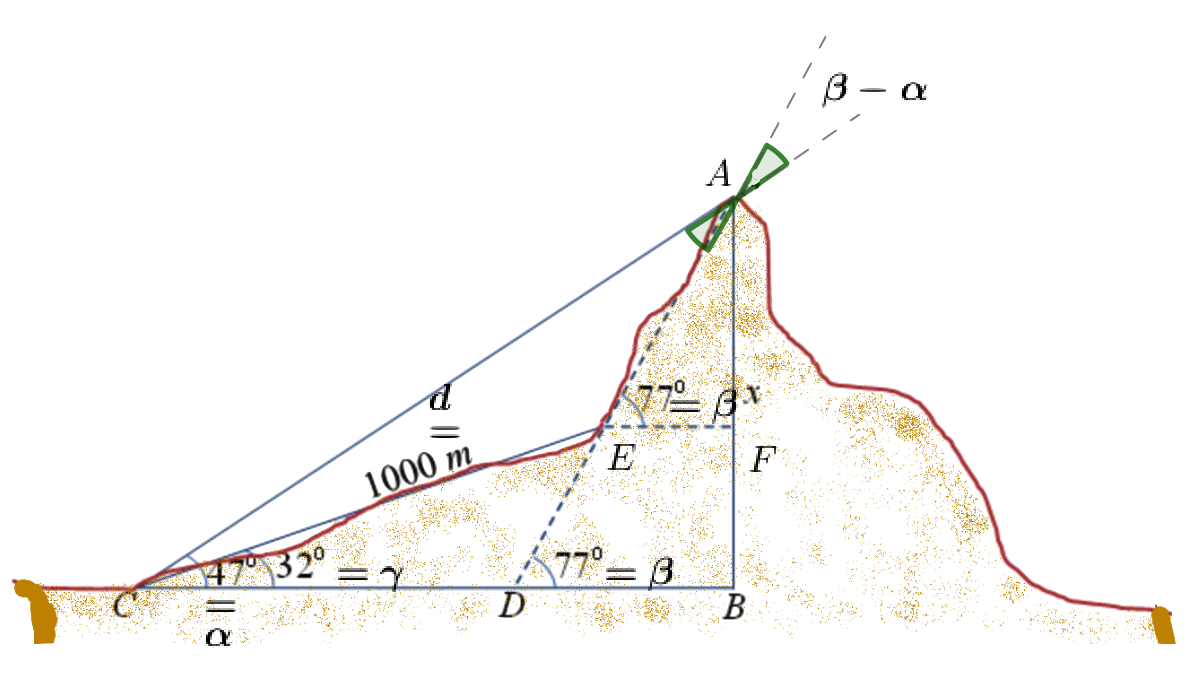
\includegraphics[width=.5\textwidth]{img-triang/triang19.png}
\end{figure}
\end{multicols}


\rule{250pt}{0.1pt}

\vspace{2mm} Queremos calcular $x=\overline{AB}\ $ Datos: $\ \alpha=\widehat{ACB}=47^o,\ \ \beta=\widehat{AEF}=\widehat{ADB}=77^o;\ \ \gamma=\widehat{ECD}=32^o,\, $ inclinación del terreno; $\  d=\overline{CD}=100\, \mathrm{m}$,

\vspace{2mm} $\widehat{CAE}=\beta-\alpha=77-47=30^o;\ \ \ \widehat{CEA}=180-(\alpha-\gamma)-(\beta-\alpha)=180+\gamma-\beta=180+32-77=135^o$

\vspace{2mm} Teorema senos triángulo $ACE:\quad \dfrac{\overline{AC}}{\sin \widehat{CEA}}=\dfrac{d}{\sin \widehat{CAE}} \ \to \ \overline{AC}=\dfrac{d\, \sin \widehat{CAE}}{\sin \widehat{CEA}}=\dfrac{15\cdot \sin 135}{\sin 30}=1414.21$

\vspace{2mm} Del triángulo rectángulo $ABC:\quad \sin A=\dfrac{x}{\sin 47}\ \to \ x=\overline{AC}\cdot \sin \alpha=1414-21\cdot \sin 47=1034.29\, \mathrm{m}$

	
\end{miejercicio}


%************
\begin{miejercicio}[ Aplicaciones topográficas 6/7]

\begin{multicols}{2}

Una columna está situada sobre un peñón. 
Desde un punto $C$ del suelo se ve la parte superior de la misma se ve con un ángulo de elevación de $55^o$. 
Situándonos en un punto $D$, 40 metros más cerca, se constata que dicho ángulo de elevación se transforma en $80^o$ y que el ángulo de elevación a la base de la columna es de $60^o$. ?`Cuál es la altura de la columna?
 
	\begin{figure}[H]
	\centering
	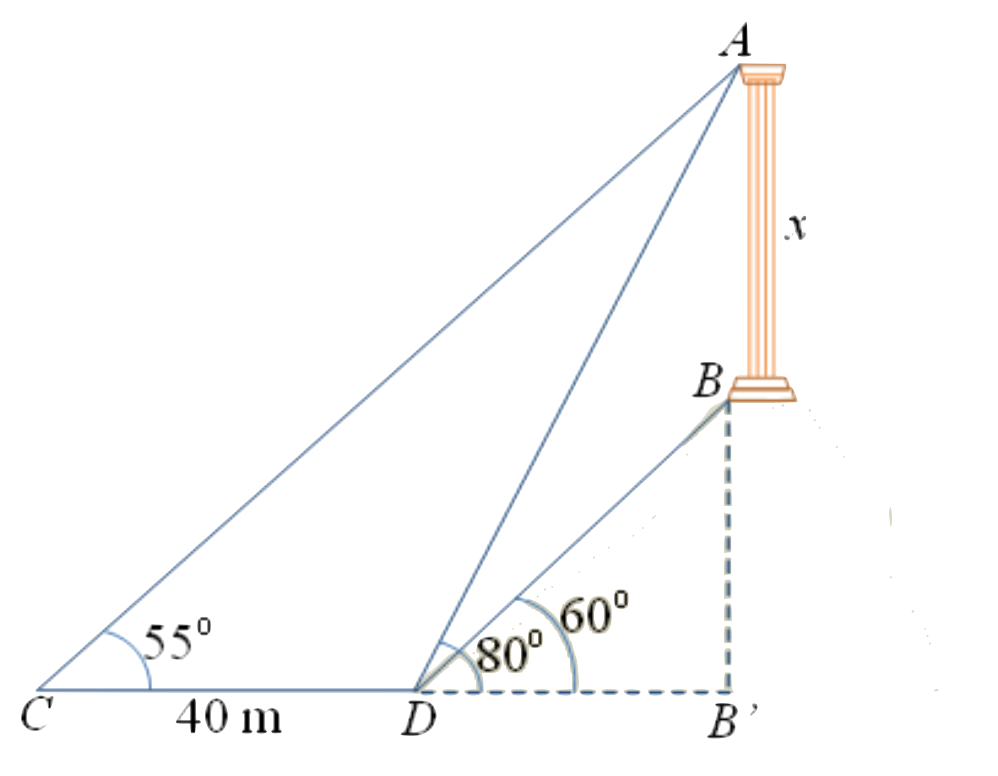
\includegraphics[width=.45\textwidth]{img-triang/triang20.png}
\end{figure}
\end{multicols}
\vspace{-6mm}
\rule{250pt}{0.1pt}

\vspace{2mm} Datos: $\ \alpha=\widehat{ACB'}=55^o;\ \ \beta=\widehat{ADB'}=80^o;\ \ \gamma=\widehat{BDB'}60^o; \ \ d=\overline{CD}=40\, \mathrm{m}\, . \ \ $  Queremos determinar $\ \ x=\overline{AB}$

\vspace{2mm} $\widehat{CAD}=180-55-(180-80)=25^o \ \to \ $ Triángulo $ ACD:$

\vspace{2mm} $\dfrac{\overline{AD}}{\sin \alpha}=\dfrac{d}{\sin \widehat{CAD}} \ \to \ \overline{AD}=\dfrac{d\, \sin \alpha}{\sin \widehat{CAD}}=\dfrac{40\cdot \sin 55}{\sin 25}=77.13$

\vspace{2mm} $\widehat{ADB}=80-60=20^o;\quad \widehat{DB'B}=180-90-60=30^o \ \to \ \widehat{DBA}=180-30=150^o \to \ $ 

\vspace{2mm}$\to \ $ Triángulo $ ABD \ \to \ 
\dfrac{\overline{AD}}{\sin \widehat{DBA}}=\dfrac{x}{\sin \widehat{ADB}} \ \to \ $

\vspace{2mm} $\to \ x=\dfrac{\overline{AD}\cot \sin \widehat{ADB}}{\sin \widehat{DBA}}=\dfrac{77.13\cdot \sin 20}{\sin 150}=53.03\, \mathrm{m} \ $ altura de la columna.

\end{miejercicio}


%************
\begin{miejercicio}[ Aplicaciones topográficas 7/7]

\begin{multicols}{2}

Para calcular la distancia entre dos puntos inaccesibles $A$ y $B$ se ha medido una base $\overline{CD}$ de $240$ metros. y los ángulos $\widehat {DCA}=106^o$, $\widehat{DCB}=39^o$, $\widehat{CDB}=122^o$, $\widehat{CDA}=41^o$.

\vspace{2mm} Calcular la distancia entre $A$ y $B$.
 
	\begin{figure}[H]
	\centering
	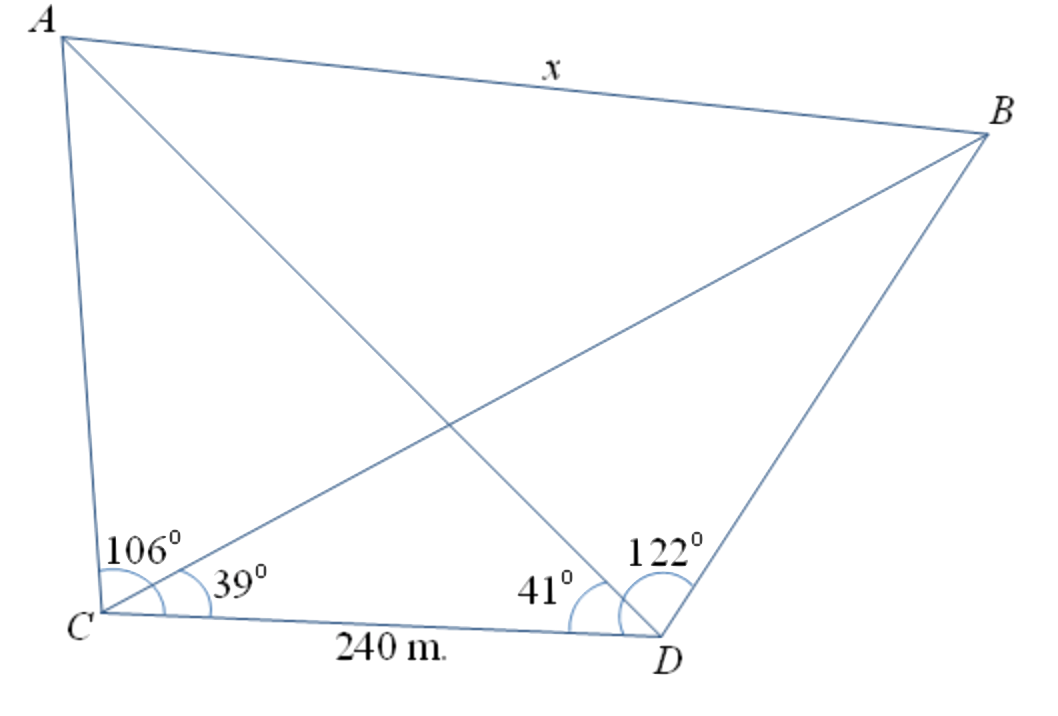
\includegraphics[width=.45\textwidth]{img-triang/triang21.png}
\end{figure}
\end{multicols}
\vspace{-8mm}

\rule{250pt}{0.1pt}

\vspace{2mm} --- Triángulo $ACD \ \to \ \overline{AC}\, , \  $ teorema de senos:

\vspace{2mm} $\widehat{CDA}=180-106-41=33^o$

\vspace{2mm} $\dfrac{\overline{AC}}{\sin \widehat{CDA}}=\dfrac{\overline{CD}}{\sin \widehat{CAD}} \ \to \ 
\overline{AC}= \dfrac{\overline{CD}\cdot \sin \widehat{CDA}}{\sin \widehat{CAD}}=\dfrac{240\cdot \sin 41}{\sin 33}=289.1$



\vspace{6mm} --- Triángulo $BCD \ \to \ \overline{CB}\, , \  $ teorema de senos:

\vspace{2mm} $\widehat{CBD}=180-122-39=19^o$

\vspace{2mm} $\dfrac{\overline{BC}}{\sin \widehat{CBD}}=\dfrac{\overline{CD}}{\sin \widehat{CBD}} \ to \ \overline{AC}=\dfrac{\overline{CD}\cdot \sin \widehat{CDB}}{\sin \widehat{CBD}}= \dfrac{40\cdot \sin 122}{\sin 19}=325.26 $

\vspace{6mm} --- Triángulo $ABD \ \to \ x=\overline{AB}\, , \  $ teorema de cosenos:

\vspace{2mm} $x^2=\overline{AB}^2=\overline{AC}^2+\overline{BC}^2-2\overline{AC}\cdot \overline{BC}\cdot \cos \widehat{ACB}=289.1^2+325.16^2-2\cdot 289.1\cdot 325.16\cdot \cos 67 \ \to $

\vspace{2mm} $\to \ x=577.2\, \mathrm{m}\ $ distancia desde $A$ hasta $B$.

\vspace{2mm}

\vspace{2mm}

	
\end{miejercicio}



%************
\begin{miejercicio}

Las tangentes trazadas desde el punto $P$ exterior a una circunferencia de centro $\mathcal O$ y de $14 \, \mathrm{cm}$ de radio forman un ángulo de $32^o$. Calcular:

a) La distancia de $P$ al centro de la circunferencia.

b) La longitud de la cuerda que une los puntos de tangencia.

\rule{250pt}{0.1pt}

\begin{figure}[H]
	\centering
	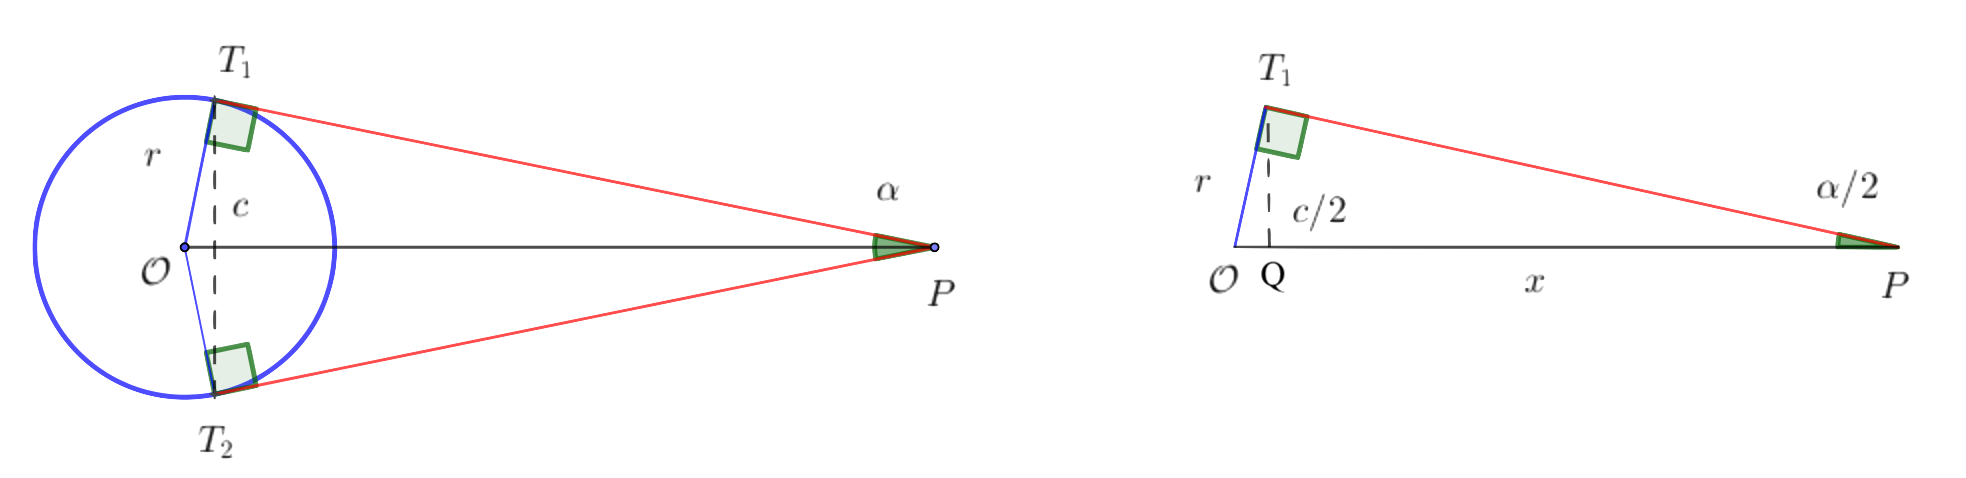
\includegraphics[width=1\textwidth]{img-triang/triang22.png}
\end{figure}

$r=14\, \mathrm{cm},\quad \alpha=32^o \ \to \ \alpha/2=16^o \quad \to \quad x\, ?\, , \ \ c\, ?$

\vspace{2mm} La recta tangente a una circunferencia y el radio son, siempre, \emph{perpendiculares}.

\vspace{2mm} Teorema de senos en el triángulo $T\mathcal O P$:

\vspace{2mm} $\dfrac{x}{\cancelto{1}{\sin 90^o}}=\dfrac{r}{\sin(\alpha/2)} \ \to \ x=\dfrac{14}{\sin 16}=50.8\, \mathrm{cm}$

\vspace{2mm} \textcolor{gris}{De otro modo:\ $\quad T\mathcal OP \, $ es triángulo rectángulo en $P \ \to \ \sin \alpha/2 = \dfrac{r}{x}=\dfrac{14}{x}=\sin 16 \ \to $}

\vspace{2mm} \textcolor{gris}{$\to \ r=14\cdot \sin 16=50.8\, \mathrm{cm}$}

\vspace{2mm} $\widehat{T\mathcal O P}=180-90-16=74$

\vspace{2mm} Por construcción, el triángulo $\mathcal O QT$ es rectángulo en $Q$, por lo que

\vspace{2mm} $\sin \widehat{T\mathcal O Q}=\dfrac{c/2}{r} \ \to \ c=2r\sin \widehat{T\mathcal O Q}=2\cdot 14\cdot \sin 74=26.9\, \mathrm{cm} $ 

\vspace{2mm}

\vspace{2mm}
\end{miejercicio}

%************
\begin{miejercicio}

Demuestra que el área de cualquier cuadrilátero es igual a la mitad del producto de sus diagonales por el seno del ángulo que forman.

\rule{250pt}{0.1pt}

\begin{multicols}{2}

$\overline{AC}=d_1$, $\overline{BD}=d_2$, $alpha$ ángulo entre diagonales. $h$ y $h'$ altura de $B$ y $D$ sobre $\overline{AC}$

$y=\overline{BO}$, $d_2-y=\overline{DO}$

$\mathcal A=\mathcal A_{ABC}+\mathcal A_{ADC}=\dfrac 1 2 d_1 h + \dfrac 1 2 d_1 h'$

\vspace{2mm} Triángulo rectángulo $BB'\mathcal O:\ \ \sin \alpha=\dfrac h y \ \to \ h=y\, \sin \alpha$

\vspace{2mm} Triángulo rectángulo $DD'\mathcal O:\ \ \sin \alpha=\dfrac {h'}{d_2-y} \ \to \ h'=(d_2-y)\, \sin \alpha$

\begin{figure}[H]
	\centering
	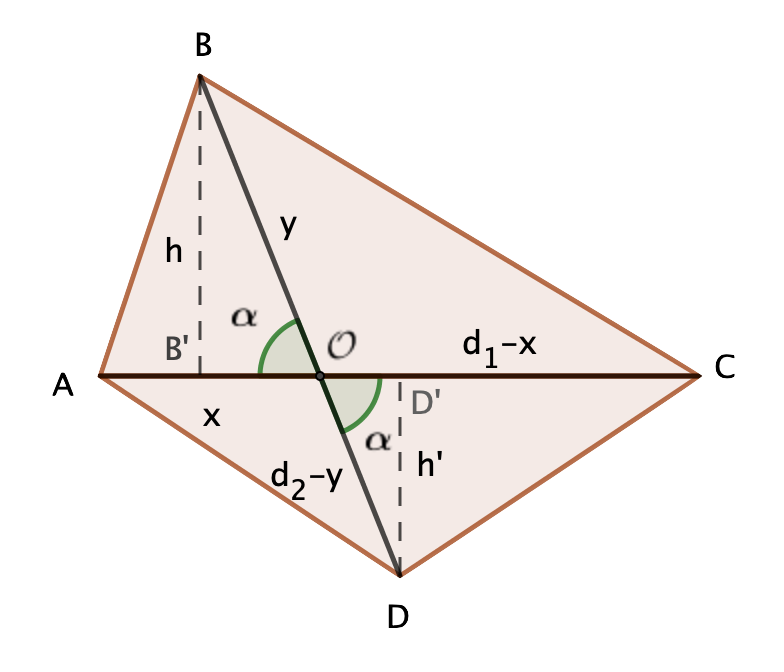
\includegraphics[width=.5\textwidth]{img-triang/triang23.png}
\end{figure}
	
\end{multicols}


$\mathcal A= \dfrac 1 2 d_1 y \sin \alpha + \dfrac 1 2 d_1 (d_2-y) \sin \alpha= \dfrac 1 2 d_1 \sin \alpha \, (y-(d_2-y))= \dfrac 1 2 \, d_1 \, d_2 \, \sin \alpha $ \QED
	
\end{miejercicio}



%%%%%%%%%%%%%%
\vspace{1.5cm}%%%%%%%%%%
\begin{mipropuesto}

Resuelve los siguientes triángulos $\quad$ \textcolor{gris}{(un dibujo, en cada caso, será de ayuda)}

\begin{multicols}{2}
\begin{enumerate}[a) ]
\item  a = 12 cm; b = 16 cm; c = 10 cm
\item  b = 22 cm; a = 7 cm; C = 40$^o$
\item  b = 4 cm; c = 3 cm; A = 105$^o$
\item  a = 4 m; B = 45$^o$; C = 60$^o$
\item  b = 5 m; A = C = 35$^o$
\item  a = b = 10 cm; C = 40$^o$
\item  a = 5 cm; A = 75$^o$; B = 45$^o$
\item  a = 16 cm; A = 90$^o$; C = 30$^o$
\item  a=3 m; b=8 m; A=25$^o$
\item  a=12.6 m;\ b=26.4 m;\ B=124.6$^o$
\item  a=82.6 m; b=11.5 m; A=28.4$^o$
\item  a=15 cm; b=11 cm; B=30$^o$
\end{enumerate}
\end{multicols}
	
\end{mipropuesto}
\vspace{-8mm}
\begin{flushright}
\begin{footnotesize} \textcolor{gris}{\rotatebox{180}{ $l)\quad$ Dos soluciones: $\quad A_1=43^o;\ C_1=107^o;\ c_1=21\, \mathrm{cm};\quad A_2=137^o;\ C_2=13^o;\ c_2=4.9\, \mathrm{cm}$ }}	\end{footnotesize}
\end{flushright}

\vspace{-10mm}
\begin{flushright}
\begin{footnotesize} \textcolor{gris}{\rotatebox{180}{ $k)\quad $ Dos soluciones: $\quad B_1=40.9^o;\ C_1=111.0^o;\ c_1=163.9\, \mathrm{m};\quad b_2=139.2^o;\ C_2=12.9^o;\ c_2=39.1\, \mathrm{m}$ }}	\end{footnotesize}
\end{flushright}

\vspace{-10mm}
\begin{flushright}
\begin{footnotesize} \textcolor{gris}{\rotatebox{180}{ $i)\quad $ No hay solución; $\qquad j)\quad A=23.1^o;\ C=32.3^o;\ c=17.1\, \mathrm{m}$ }}	\end{footnotesize}
\end{flushright}


\vspace{-10mm}
\begin{flushright}
\begin{footnotesize} \textcolor{gris}{\rotatebox{180}{ $g)\quad C=60^o;\ b=3.7\, \mathrm{cm};\ c=4.5\, \mathrm{cm};\qquad h)\quad B=60^o;\ c=8\, \mathrm{cm};\ b=13.9\, \mathrm{cm}$ }}	\end{footnotesize}
\end{flushright}

\vspace{-10mm}
\begin{flushright}
\begin{footnotesize} \textcolor{gris}{\rotatebox{180}{ $e)\quad B=110^o;\ a=c=3.1\, \mathrm{m} \ \text{(isósceles)};\qquad f)\quad A=B=70^o;\ c=6.8\, \mathrm{cm} \ \text{(isósceles)}$ }}	\end{footnotesize}
\end{flushright}

\vspace{-10mm}
\begin{flushright}
\begin{footnotesize} \textcolor{gris}{\rotatebox{180}{ $c)\quad a=5.6\, \mathrm{m};\ B=43.7^o;\ C=31.3^o;\qquad d)\quad A=75^0;\ b=2.0\, \mathrm{m};\  c=3.6\, \mathrm{m}$ }}	\end{footnotesize}
\end{flushright}

\vspace{-10mm}
\begin{flushright}
\begin{footnotesize} \textcolor{gris}{\rotatebox{180}{ $a)\quad A=48.5^o;\ B=98.9^o;\ C=38.6^o;\qquad b)\quad c=17.2\, \mathrm{cm};\ A=15.1^o;\ B=124.9^o$ }}	\end{footnotesize}
\end{flushright}


%%%%%%%%%%%%%%
%\vspace{1cm}
\begin{mipropuesto}

A dos puertos, separados longitudinalmente por 20 Km, se reciben a la vez señales de socorro de un barco que se encuentra en alta mar. El puerto A recibe la señal con un ángulo de 75$^o$ mientras que el B lo recibe con un  ́ángulo de 60$^o$. También se sabe que el barco está entre los dos puertos, pero perdido dentro del mar, y se pide calcular a qué distancia se encuentra de ellos.	
\end{mipropuesto}

\vspace{-8mm}
\begin{flushright}
\begin{footnotesize} \textcolor{gris}{\rotatebox{180}{ A 27.32 km de A y 24.49 km de B. }}	\end{footnotesize}
\end{flushright}

%%%%%%%%%%%%%%
%\vspace{1cm}
\begin{mipropuesto}
	
	Un barco observa la luz de dos faros de la costa, que se encuentran separados por una distancia de 40 Km, y las luces inciden en dicho barco con un ángulo de 33$^o$. El capitán sabe que se encuentra a 50 Km del faro más cercano. Se pide, calcular la distancia desde el barco al otro faro y los ángulos del triángulo formado.
\end{mipropuesto}

\vspace{-8mm}
\begin{flushright}
\begin{footnotesize} \textcolor{gris}{\rotatebox{180}{ $42.9^o,\ \ 104.1^o,\ \ 71.232 \, \mathrm{km}$ }}	\end{footnotesize}
\end{flushright}

%%%%%%%%%%%%%%
%\vspace{1cm}
\begin{mipropuesto}

Dos barcos pesqueros que se encuentran faenando y separados por una distancia de 100 Km empiezan a recibir una señal de socorro. Rápidamente se ponen en contacto los capitanes de ambos barcos para situar el origen de la señal, para ello trazan una línea entre ambos, y sobre esa línea uno de ellos recibe la señal con un ángulo de 70$^o$, mientras que el otro la recibe con un ángulo de 60$^o$. Calcula las distancias que separan a estos dos barcos del origen de la señal.
	
\end{mipropuesto}

\vspace{-8mm}
\begin{flushright}
\begin{footnotesize} \textcolor{gris}{\rotatebox{180}{ 122.668 Km de A y 113.052 km de B. }}	\end{footnotesize}
\end{flushright}

%%%%%%%%%%%%%%
%\vspace{1cm}
\begin{mipropuesto}
	
	Dos circunferencias cuyos radios son 10 y 12 cm se cortan. El ángulo que forman las tangentes respectivas en el punto de intersección mide 40$^o$.  Halla la distancia entre los dos centros de la circunferencia.
\end{mipropuesto}

\vspace{-8mm}
\begin{flushright}
\begin{footnotesize} \textcolor{gris}{\rotatebox{180}{ 20.7 cm }}	\end{footnotesize}
\end{flushright}

%%%%%%%%%%%%%%
%\vspace{1cm}
\begin{mipropuesto}
	
	Dos amigos aficionados a la astronomía y, que se encuentran separados por una distancia de 1000 Km, están observando un foco de luz que, por una causa desconocida había aparecido en el firmamento en medio de las estrellas. Ese objeto luminoso se confunde con lo que sería una nueva estrella desconocida, por lo que deciden investigar. Uno de ellos apunta con su telescopio bajo un ángulo de 85$^o$, mientras que el otro lo hace con un ángulo de 87$^o$. Calcular la distancia de cada uno de ellos al objeto en cuestión. ?`Se tratará de una estrella?
\end{mipropuesto}

\vspace{-8mm}
\begin{flushright}
\begin{footnotesize} \textcolor{gris}{\rotatebox{180}{ 7157.95 km de A y 7175.45 km de B. Obviamente, no se trata de una estrella. }}	\end{footnotesize}
\end{flushright}

%%%%%%%%%%%%%%
%\vspace{1.5cm}%%%%%%%%%%
\begin{mipropuesto}

Para hallar la distancia entre dos barcos en el mar C y D fijamos dos puntos A y B en la playa, tales que AB = 500 m y medimos los siguientes ángulos con el teodolito: CAD = 50$^o$,           DAB = 63$^o$,           ABC = 38$^o$ y           CBD = 57$^o$
	
\end{mipropuesto}

\vspace{-8mm}
\begin{flushright}
\begin{footnotesize} \textcolor{gris}{\rotatebox{180}{ 1042m }}	\end{footnotesize}
\end{flushright}

%%%%%%%%%%%%%%
%\vspace{1cm}
\begin{mipropuesto}
	
	Un faro de 20 m de altura está colocado sobre un promontorio. Un barco ve el pedestal bajo un ángulo de 15$^o$ y el faro, bajo un ángulo de 40$^o$. Calcula la altura del promontorio.
\end{mipropuesto}

\vspace{-8mm}
\begin{flushright}
\begin{footnotesize} \textcolor{gris}{\rotatebox{180}{ 7.32 m }}	\end{footnotesize}
\end{flushright}

%%%%%%%%%%%%%%
%\vspace{1cm}
\begin{mipropuesto}
	
	Un solar tiene forma de triángulo y se conocen dos lados que miden 36 m y 46 m, y el ángulo que forman es de 125$^o$. El metro cuadrado vale 100 €. Calcula el valor del solar.
\end{mipropuesto}

\vspace{-8mm}
\begin{flushright}
\begin{footnotesize} \textcolor{gris}{\rotatebox{180}{ 67825.79 \euro }}	\end{footnotesize}
\end{flushright}

%%%%%%%%%%%%%%
%\vspace{1cm}
\begin{mipropuesto}
	
	Dos fuerzas de 18 N y 30 N actúan sobre un punto formando un ángulo de 45$^o$. Calcula la intensidad de la resultante y el ángulo que forma con cada una de las fuerzas.
\end{mipropuesto}

\vspace{-8mm}
\begin{flushright}
\begin{footnotesize} \textcolor{gris}{\rotatebox{180}{ 44.6N, 16.6$^o$, 28.4$^o$ }}	\end{footnotesize}
\end{flushright}

%%%%%%%%%%%%%%
%\vspace{1cm}
\begin{mipropuesto}
	
	Dos circunferencias secantes tienen radios de 6 cm y 10 cm. Sus tangentes comunes forman un ángulo de 40$^o$. Calcula la distancia entre sus centros.
\end{mipropuesto}

\vspace{-8mm}
\begin{flushright}
\begin{footnotesize} \textcolor{gris}{\rotatebox{180}{ 11.7 cn }}	\end{footnotesize}
\end{flushright}

%%%%%%%%%%%%%%
%\vspace{1cm}
\begin{mipropuesto}
	
	Uno de los lados de un triángulo mide el doble que otro, y el ángulo comprendido entre ellos mide 60$^o$. Halla los otros ángulos.
\end{mipropuesto}

\vspace{-8mm}
\begin{flushright}
\begin{footnotesize} \textcolor{gris}{\rotatebox{180}{ 30$^o$ y 90$^o$ }}	\end{footnotesize}
\end{flushright}

%%%%%%%%%%%%%%
%\vspace{1cm}
\begin{mipropuesto}
	
	Halla el ángulo que forman dos caras contiguas de un tetraedro regular de arista $x$.
\end{mipropuesto}

\vspace{-8mm}
\begin{flushright}
\begin{footnotesize} \textcolor{gris}{\rotatebox{180}{ 70.53$^o$ }}	\end{footnotesize}
\end{flushright}

%%%%%%%%%%%%%%
%\vspace{1cm}
\begin{mipropuesto}
	
	Sobre un montículo de 8 m de altura hemos instalado una antena de 10 m de longitud. ?`Desde qué distancia se verán bajo ángulos iguales el montículo y la antena?
\end{mipropuesto}

\vspace{-8mm}
\begin{flushright}
\begin{footnotesize} \textcolor{gris}{\rotatebox{180}{ 24 m }}	\end{footnotesize}
\end{flushright}

%%%%%%%%%%%%%%
%\vspace{1cm}
\begin{mipropuesto}
	
	Sean A, B y C los tres vértices de un triángulo equilátero de lado 3 cm y P el punto del lado AB que está a 1 cm del vértice A. ?`Cuál es la longitud del segmento CP?
\end{mipropuesto}

\vspace{-8mm}
\begin{flushright}
\begin{footnotesize} \textcolor{gris}{\rotatebox{180}{ $\sqrt{7}$ cm }}	\end{footnotesize}
\end{flushright}

%%%%%%%%%%%%%%
%\vspace{1cm}
\begin{mipropuesto}
	
	
En una cartulina cuadrada de 24 cm de lado, ?`se puede dibujar la circunferencia circunscrita a un triángulo de lados 15, 20 y 25 cm?
\end{mipropuesto}

\vspace{-8mm}
\begin{flushright}
\begin{footnotesize} \textcolor{gris}{\rotatebox{180}{ $2R=25$ cm; no se puede dibujar. }}	\end{footnotesize}
\end{flushright}

%%%%%%%%%%%%%%
%\vspace{1cm}
\begin{mipropuesto}
	
	De un triángulo sabemos que la suma de las longitudes de los lados a y b es de 11 m, que el ángulo C opuesto al tercer lado vale 30$^o$ y que su área es de 7 m$^2$.Calcula la longitud de cada uno de los lados del triángulo y  los ángulos.
\end{mipropuesto}

\vspace{-8mm}
\begin{flushright}
\begin{footnotesize} \textcolor{gris}{\rotatebox{180}{ Hay dos soluciones: $a=(b=)7; \ b=(a=)=4; \ c=4.06;\ A=(B=)=29.51^o;\ B=(A=)=120.49^0$ }}	\end{footnotesize}
\end{flushright}

\vspace{-8mm}
\begin{flushright}
\begin{footnotesize} \textcolor{gris}{\rotatebox{180}{ Plantea un sistema con la suma de lados y el área. }}	\end{footnotesize}
\end{flushright}



%%%%%%%%%%%%%%
%\vspace{1cm}
\begin{mipropuesto}
	
	Una estatua y su pedestal se ven bajo ángulos de 13$^o$ y 30$^o$ respectivamente. Si retrocedemos 20 m el conjunto se ve bajo un ángulo de 11$^o$. Calcula la altura del pedestal y de la estatua.
\end{mipropuesto}

\vspace{-8mm}
\begin{flushright}
\begin{footnotesize} \textcolor{gris}{\rotatebox{180}{ 1.87 m }}	\end{footnotesize}
\end{flushright}

%%%%%%%%%%%%%%
%\vspace{1cm}
\begin{mipropuesto}
	
	Entre dos transeúntes, situados uno detrás del otro, hay una distancia de 30 m. El más alejado ve un edificio bajo un ángulo de 50o. Desde la azotea del edificio un vigilante ve a estos transeúntes bajo un ángulo de 24o. Calcula la altura del edificio.
\end{mipropuesto}

\vspace{-8mm}
\begin{flushright}
\begin{footnotesize} \textcolor{gris}{\rotatebox{180}{ 54.3 m }}	\end{footnotesize}
\end{flushright}

%%%%%%%%%%%%%%
%\vspace{1cm}
\begin{mipropuesto}
	
	Desde dos puntos A y B, distantes 750 m, y situados en la misma orilla del río se ven dos puntos C y D en la otra orilla. Se han medido los siguientes ángulos: BAD=68$^o$, BAC=32$^o$, ABD=45$^o$ y ABC=72$^o$. Calcula la distancia entre C y D.
\end{mipropuesto}

\vspace{-8mm}
\begin{flushright}
\begin{footnotesize} \textcolor{gris}{\rotatebox{180}{ 432.5 m }}	\end{footnotesize}
\end{flushright}

%%%%%%%%%%%%%%
\vspace{1cm}



\begin{myexampleblock}{Star Wars $\quad$ \emph{(ejercicio propuesto)} }
	
\vspace{2mm}La Estrella de la Muerte es una estación espacial esférica perteneciente al Imperio Galáctico con capacidad suficiente para reducir un planeta a polvo cósmico. Sin embargo, tal portento tecnológico tiene un punto débil, un pequeño resquicio al que se accede a través de un pasillo situado en su superficie y que está señalado en el plano de la figura como `punto D'.

\vspace{2mm}La Alianza Rebelde elige a Luke Skywalker para internar alcanzar dicho punto con su nave X-Wing. Junto a él viaja, después de pensarlo mucho, su amigo Han Solo pilotando el mítico Halcón Milenario. Ambos se dirigen en línea recta hacia el punto D.

\vspace{2mm}No obstante, el malvado Darth Vader se entera de los planes de la Alianza y también avanza en linea recta hacia el punto D en su Tie-Fighter con la finalidad de protegerlo.

\begin{figure}[H]
	\centering
	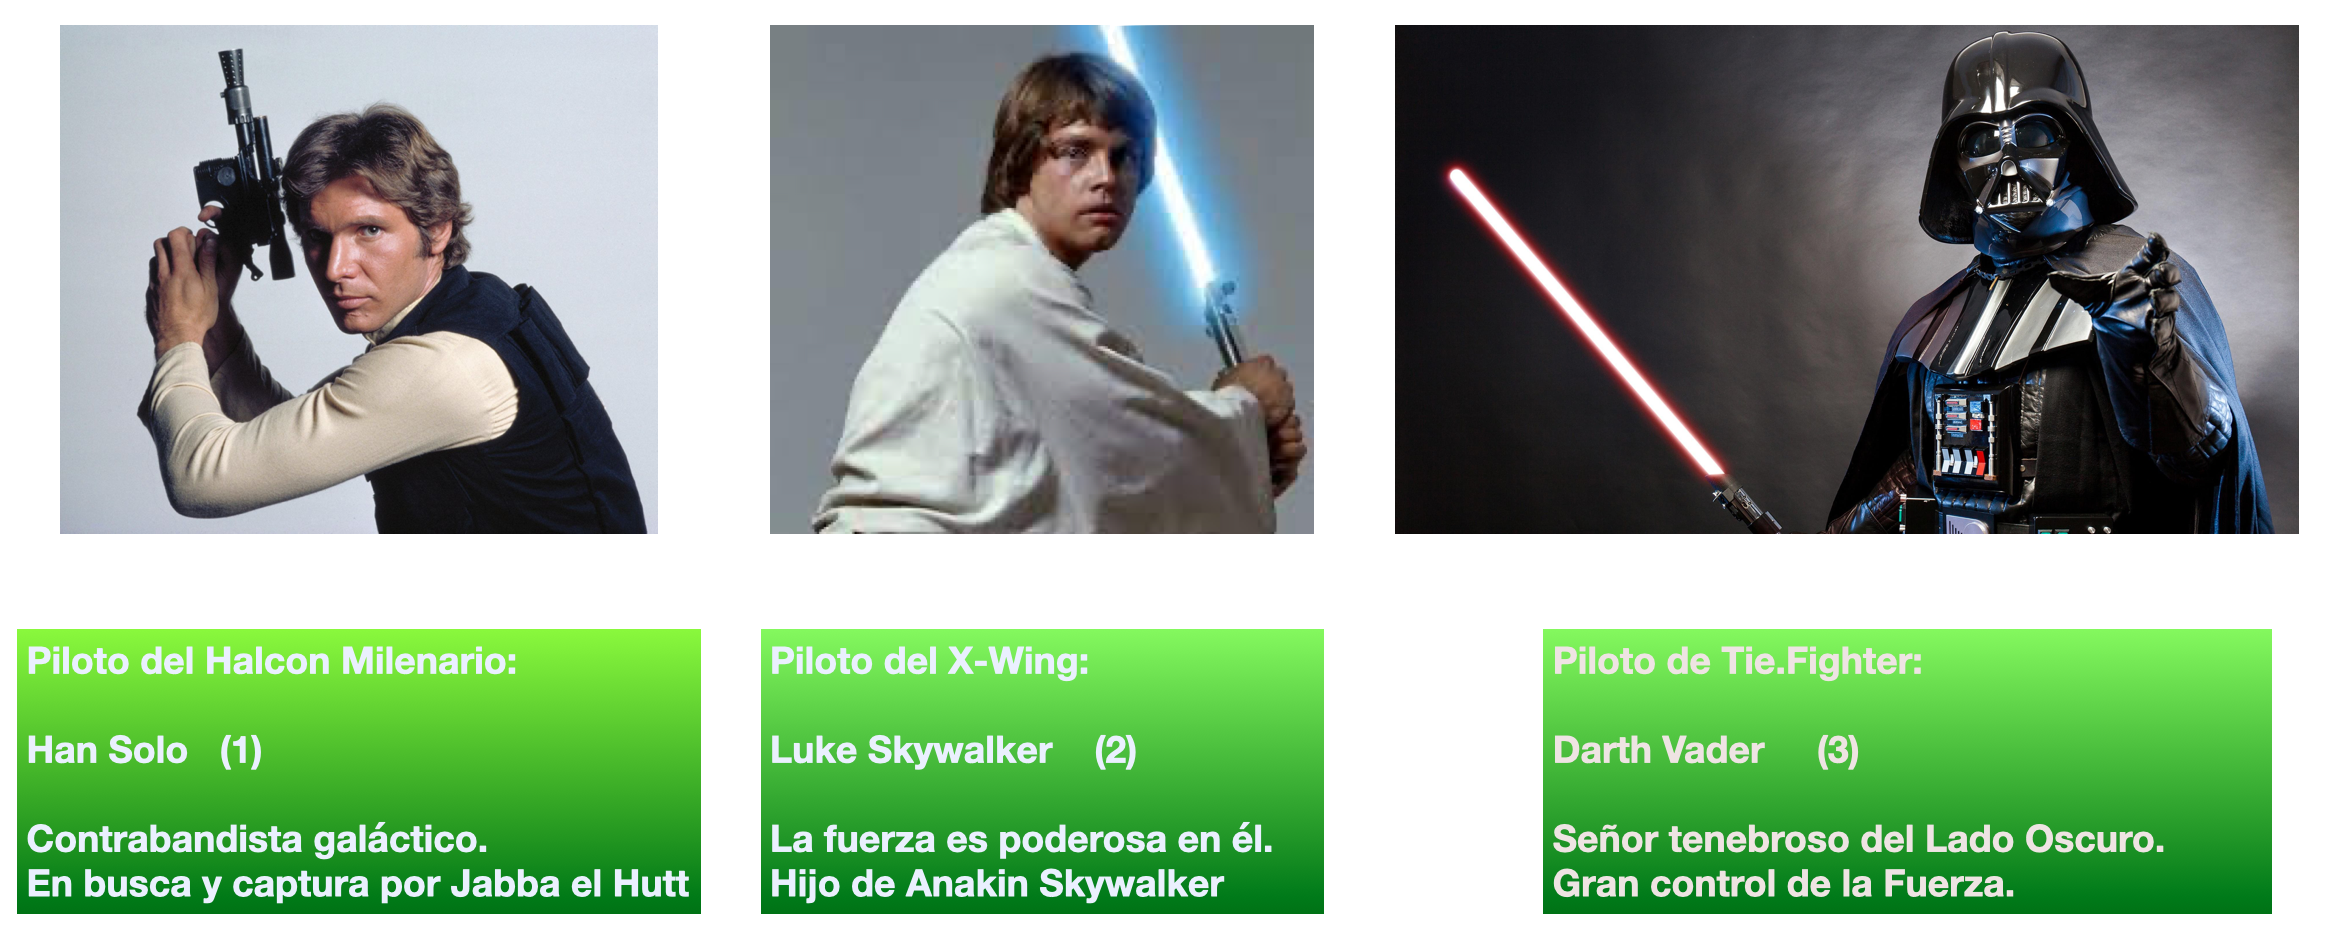
\includegraphics[width=.75\textwidth]{img-triang/sw5.png}
\end{figure}

En el momento en que nos encontramos se detalla en el gráfico, con las tres naves alineadas. Además, conocemos los siguientes datos.

\begin{itemize}
\item Radio de la Estrella de la Muerte: 80 km.
\item Distancia de Han Solo al centro de la Estrella de la Muerte: 500 km.
\item Ángulo formado por Han Solo, centro de la Estrella de la Muerte y punto D: $53.13^o$
\item Ángulo formado por Han Solo, punto D y Darth Vader: $90^o$.
\item Ángulo formado por punto D, Luke Skywalker y Darth Vader: $90^o$.
\item Velocidades: Halcón Milenario 50 Km/s, X-Wing 40 km/s y Tie-Fighter 42 km/s.
\end{itemize}

Calcula las distancias de cada nave al punto D, así como el tiempo que empleará cada una de ellas en llegar a él.

	\begin{figure}[H]
	\centering
	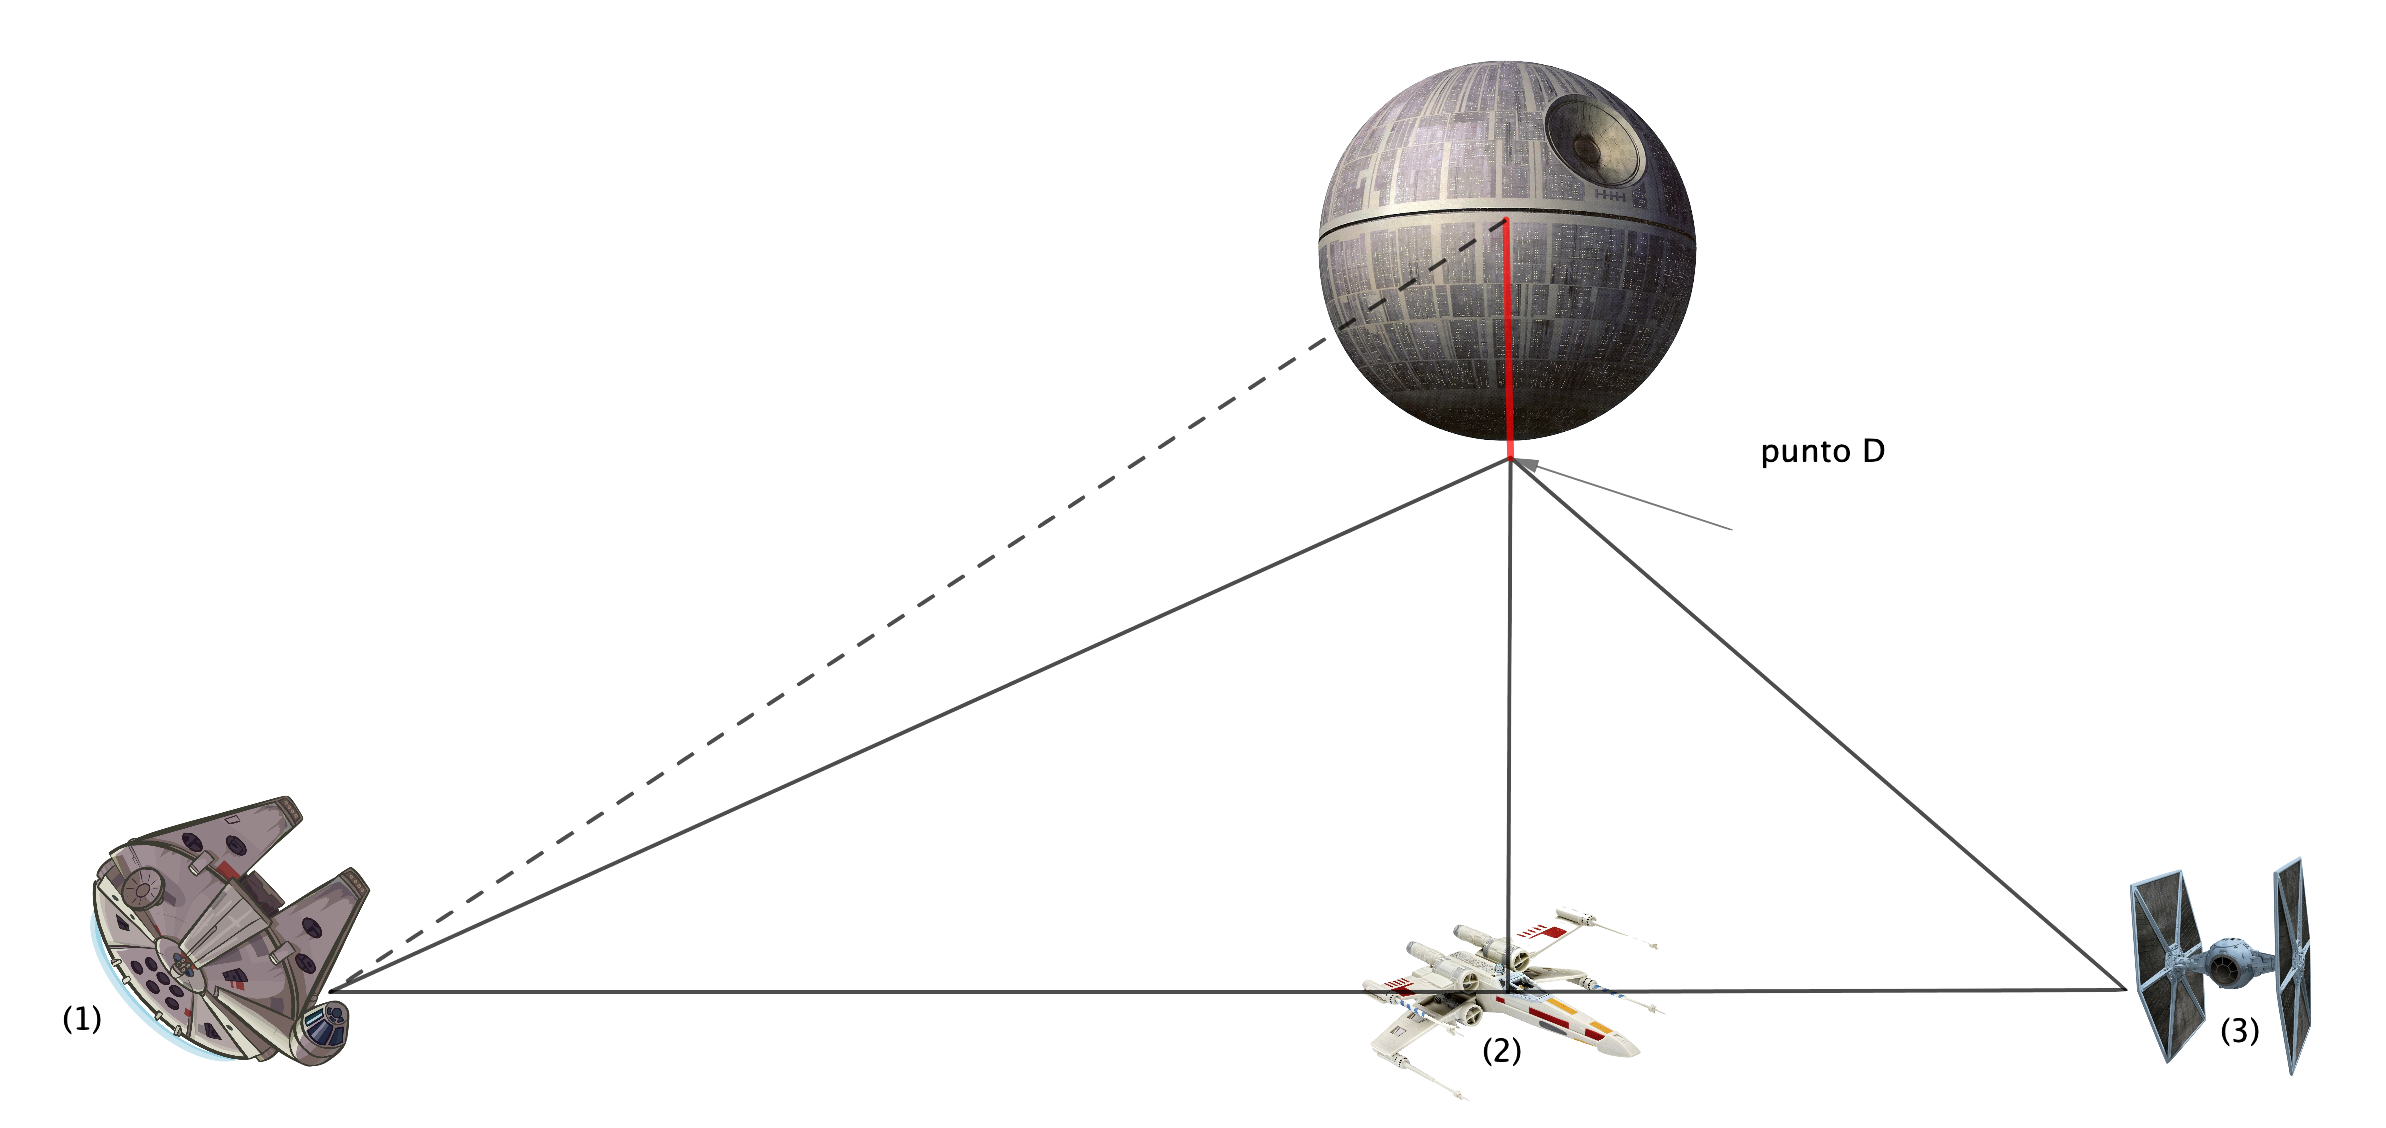
\includegraphics[width=1\textwidth]{img-triang/sw0.png}
\end{figure}

\begin{flushright}
\begin{footnotesize} \textcolor{gris}{\rotatebox{180}{ Han Solo: 456.508 km, 9.13 s; $\quad$ Luck Skywalker: 219.994 km, 5.50 s; $\quad$ Darth Vader: 251.071 km, 5,98 s. }}	\end{footnotesize}
\end{flushright}	
\end{myexampleblock}






%++++++++++++++++++++++++++++++++++++
%********************************************************************
\newpage
\vspace{1cm}
\begin{adjustwidth}{50pt}{250pt}
\begin{cuadro-naranja}
\textbf{\huge{Problemas $\boldsymbol{+}$}}\normalsize{$\, $}
\end{cuadro-naranja}	
\end{adjustwidth}

\vspace{5mm}
\begin{enumerate}[\textbf{P$\boldsymbol +$} 1. ]

%%%%
\item	En un triángulo $ABC$ se sabe que el ángulo $A$ es triple que el ángulo $B$. Si $\overline{BC}=5\, \mathrm{u}$ y $\overline{CA}=3\, \mathrm{u}$, calcula $\overline{AB}$

\vspace{-6mm}
\begin{flushright}
\begin{footnotesize} \textcolor{gris}{\rotatebox{180}{ $\alpha$ por Th. senos, $\ \to C \ $ Th. cosenos $\ \to \overline{AB}=2,27\, \mathrm{u}$ }}	\end{footnotesize}
\end{flushright}


%%%%
\item	 Sea $ABC$ un triángulo en el que $A=45^o$, $C=30^o$ y sea $D$ el punto medio del lado $BC$. Calcula la medida del ángulo $\widehat{CAD}$

\vspace{-6mm}
\begin{flushright}
\begin{footnotesize} \textcolor{gris}{\rotatebox{180}{ Th. senos a los triángulos $ACD \text{ y } ADB:\qquad  \widehat{CAD}=15^o$ }}	\end{footnotesize}
\end{flushright}


%%%%
\item	$\quad$


\begin{figure}[H]
	\centering
	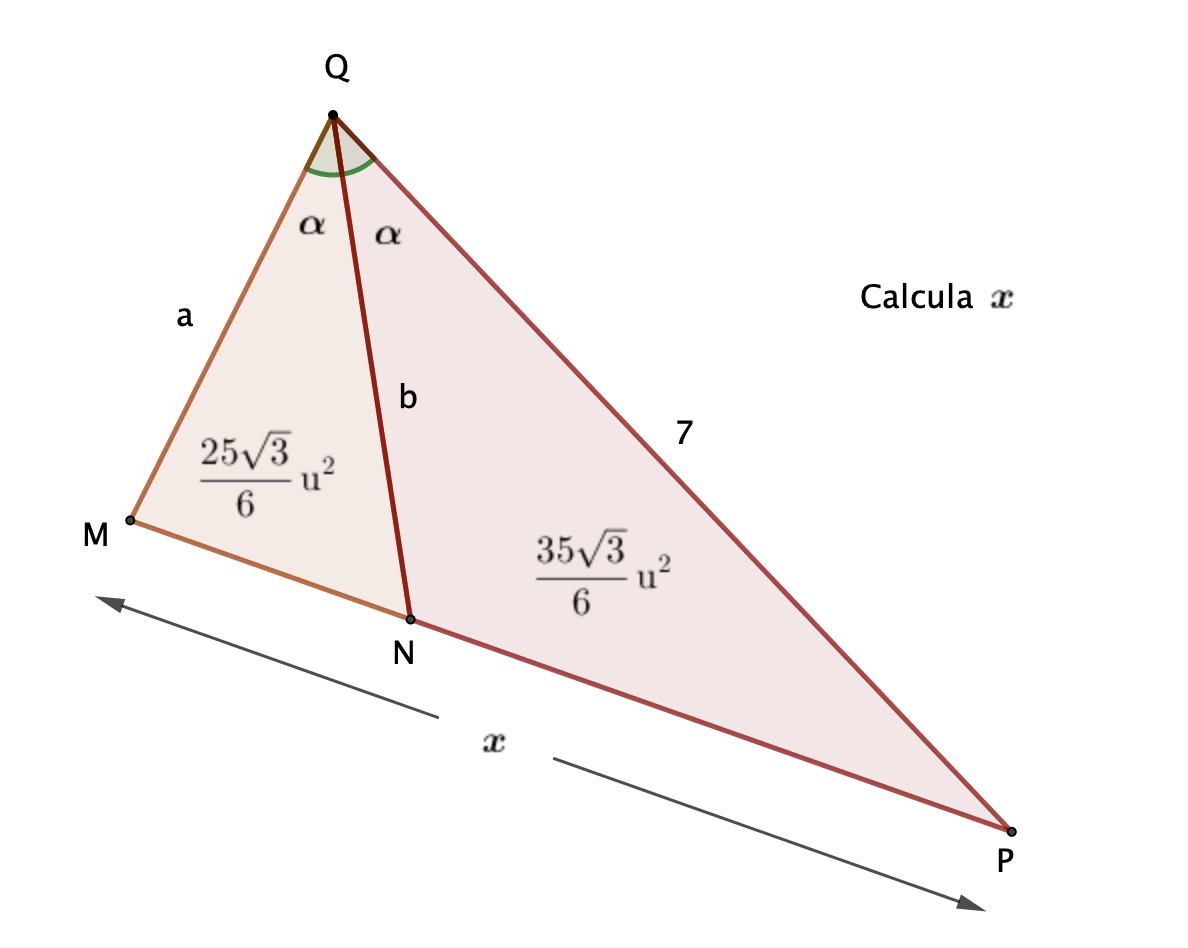
\includegraphics[width=0.45\textwidth]{img-triang/triang24.png}
\end{figure}

\vspace{-6mm}
\begin{flushright}
\begin{footnotesize} \textcolor{gris}{\rotatebox{180}{ $\mathcal A_{MNQ}\, ,\ \mathcal A_{NPQ} \  \to \ a; \quad \mathcal A_{MPQ}\ \to \ \alpha \quad \Rightarrow \quad x=8\, \mathrm{u}$ }}	\end{footnotesize}
\end{flushright}


%%%%
\item	 En un triángulo, el ángulo intermedio (ni el mayor ni el menor) mide 60$^o$. Encuentra el valor de los lados sabiendo que los dos menores se diferencian en dos unidades y los dos mayores en una unidad.

\vspace{-6mm}
\begin{flushright}
\begin{footnotesize} \textcolor{gris}{\rotatebox{180}{ En un triángulo, a mayor ángulo le corresponde mayor lado opuesto. Th. cosenos. $\qquad 5,7 \text{ y } 8\, \mathrm{u}$ }}	\end{footnotesize}
\end{flushright}

%%%%
\item	 En un triángulo, los lados son proporcionales a 5, 7 y 8. Calcula el ángulo formado por los lados mayor y menor.

\vspace{-6mm}
\begin{flushright}
\begin{footnotesize} \textcolor{gris}{\rotatebox{180}{ Th. cosenos $\qquad 60^o$ }}	\end{footnotesize}
\end{flushright}

%%%%
\item	Desde un punto del suelo, un observador divisa el punto más alto de una torre bajo un ángulo de elevación de $2\theta$, siendo la longitud de la visual de $96$ m. Si el observador avanza hacia la torre $64$ m, el nuevo ángulo de elevación es de $3\theta$. Calcula la altura de la torre.

\vspace{-6mm}
\begin{flushright}
\begin{footnotesize} \textcolor{gris}{\rotatebox{180}{ $24\sqrt{15}$ m. }}	\end{footnotesize}
\end{flushright}

%%%%
\item	 En un triángulo, los lados son tres enteros consecutivos u el ángulo mayor es doble que el menor. Calcula la longitud de los lados.

\vspace{-6mm}
\begin{flushright}
\begin{footnotesize} \textcolor{gris}{\rotatebox{180}{ Lados: $n-1,\, n,\ n+1: \qquad$ Th. senos $\ \to \cos \alpha\ \to \  $ Th. cosenos $\ n=5 \ \to \ $ lados: 4, 5 y 6 u.  }}	\end{footnotesize}
\end{flushright}


%%%%
\item	 De un puerto zarpan, simultáneamente, dos barcos con rumbos $S20^oE$ y $S40^oW$ y velocidades constantes de 25 m/s y 30 m/s, respectivamente.. Al cabo de 15 min, ?`qué distancia les separa?

\vspace{-8mm}
\begin{flushright}
\begin{footnotesize} \textcolor{gris}{\rotatebox{180}{ Th. cosenos: $\quad 25.055$ km. }}	\end{footnotesize}
\end{flushright}


\end{enumerate}


\vspace{1.5cm}%%%%%*******************


%\vspace{1cm}
\section{Resumen del tema}

\begin{tikzpicture}
	\fill [left color=red!50, right color=teal!50] (0,0) rectangle (3.5,.1);
	\fill [left color=teal!50, right color=blue!50] (3.5,0) rectangle (7.5,.1);
	\end{tikzpicture}
\vspace{0.5cm}
\begin{myblock}{Resumen \emph{``Resolución de triángulos''}}
\vspace{1mm}

\vspace{1mm} $\checkmark\ $ En cualquier triángulo, la suma de dos cualesquiera de sus lador es mayor que el tercero.

\vspace{1mm} $\checkmark\ $ La suma de los ángulos internos de un triángulo suman $180^o$

\vspace{1mm}\begin{footnotesize} $\checkmark\ $ 
\emph{Test de Pitágoras}:  Elegido el lado más grande, comparamos su cuadrado con la suma de los cuadrados de los otros dos lados; si es mayor, el triángulo es obtusángulo; si es igual, rectángulo y si es menor, el triángulo es acutángulo.	
\end{footnotesize}


\vspace{1mm} $\checkmark\ $ Teorema de senos: $\quad $ \emph{En todo triángulo el cociente entre un lado cualquiera y el seno de su ángulo opuesto es una constante}

$$ \boldsymbol{ \dfrac{a}{\sin A} \ = \  \dfrac{b}{\sin B} \ = \  \dfrac{c}{\sin D} } $$

\vspace{1mm} $\checkmark\ $ Teorema de cosenos: $\quad $ \emph{En todo triángulo, el cuadrado de un lado siempre es igual a la suma de los cuadrados de los otros dos menos el doble producto de ellos por el coseno del ángulo comprendido.}
	
	$$\boldsymbol{ a^2=b^2+c^2-2bc\cos A} \, ;  \qquad  b^2=a^2+c^2-2ac\cos B \, ; \qquad c^2=a^2+b^2-2ab\cos C $$
	
\vspace{1mm} $\checkmark\ $ Área de un triángulo $\quad$ \emph{El área de un triángulo es la mitad del producto de dos de sus lados por el seno del ángulo comprendido.}

$$ \boldsymbol{\mathcal A=\dfrac 1 2 \, a\, b\, \sin C}\, ; \qquad \mathcal A=\dfrac 1 2 \, b\, c\, \sin A\, ; \qquad \mathcal A=\dfrac 1 2 \, a\, c\, \sin B$$

\begin{figure}[H]
	\centering
	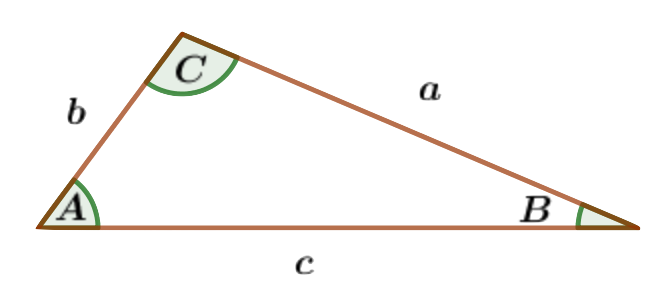
\includegraphics[width=0.4\textwidth]{img-triang/triang01.png}
	%\caption*{Nomenclatura}
\end{figure}
\end{myblock}


\begin{comment}

%*************************.  EJERCICIOS




%************
\begin{miejercicio}

Enun

\rule{250pt}{0.1pt}

\vspace{2mm}

	
\end{miejercicio}


%%%%%%%%%%%%%%
\vspace{1cm}
\begin{mipropuesto}
	
\end{mipropuesto}

\vspace{-8mm}
\begin{flushright}
\begin{footnotesize} \textcolor{gris}{\rotatebox{180}{ sol }}	\end{footnotesize}
\end{flushright}



%%%%%%%%%%%%%%%%%%%%%%%%%%%%%%%%%%%. SECCIONES

\begin{figure}[H]
	\centering
	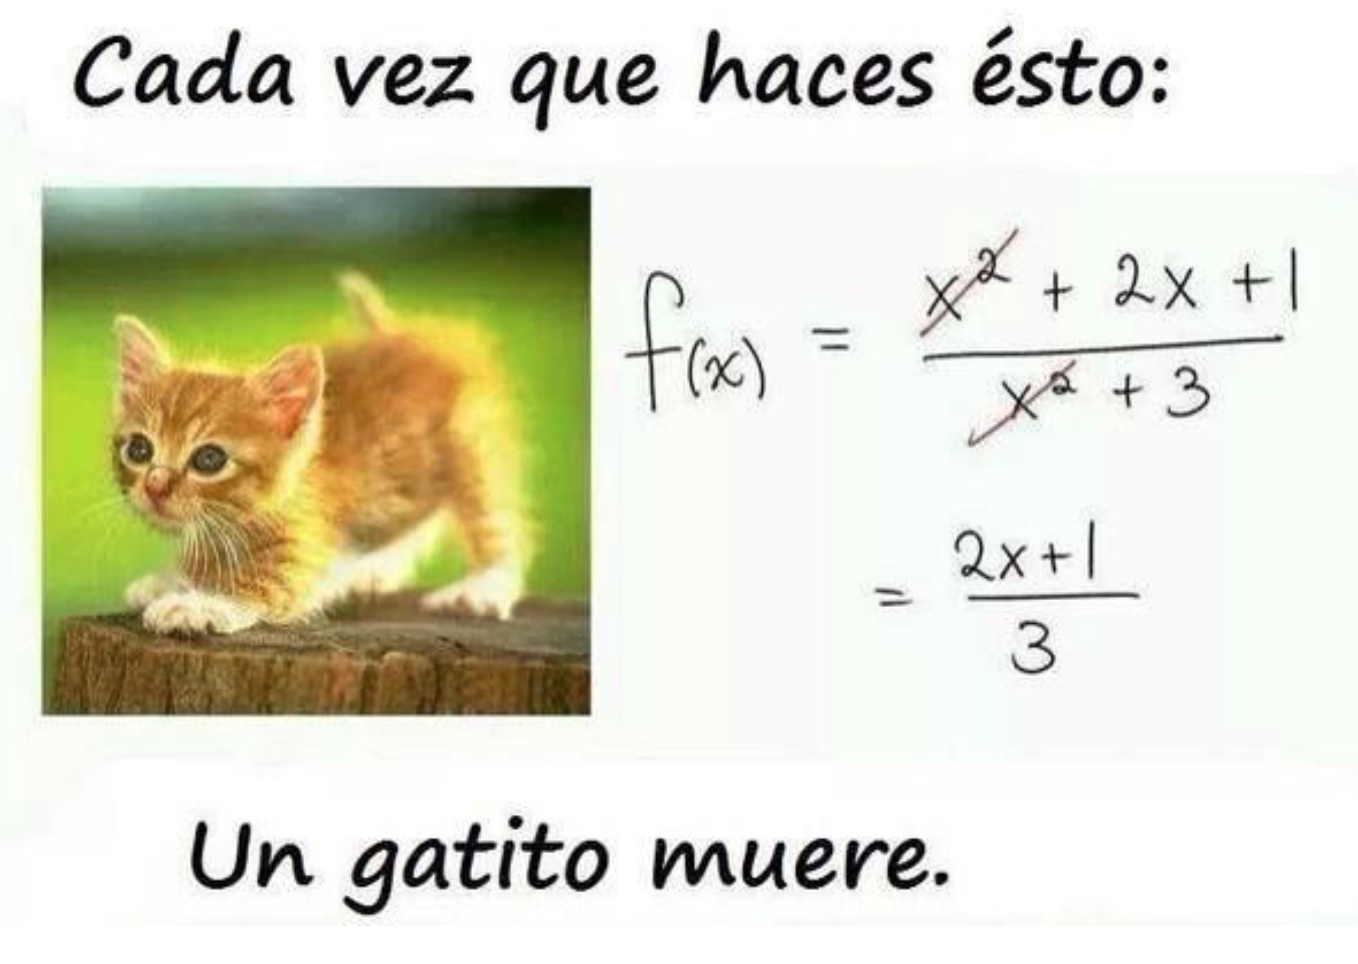
\includegraphics[width=0.35\textwidth]{img-pol/pol05.png}
\end{figure}



\chapter{texto}

\begin{tikzpicture}
	\fill [left color=red!50, right color=teal!50] (0,0) rectangle (6.5,.2);
	\fill [left color=teal!50, right color=blue!50] (6.5,0) rectangle (11.5,.2);
	\end{tikzpicture}

\vspace{1cm}
\section{texto}

\begin{tikzpicture}
	\fill [left color=red!50, right color=teal!50] (0,0) rectangle (3.5,.1);
	\fill [left color=teal!50, right color=blue!50] (3.5,0) rectangle (7.5,.1);
	\end{tikzpicture}
\vspace{0.5cm}

\subsection{texto}
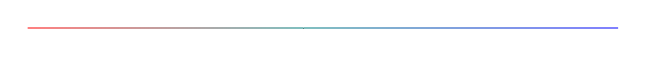
\begin{tikzpicture}
	\fill [left color=red!50, right color=teal!50] (0,0) rectangle (3.5,.01);
	\fill [left color=teal!50, right color=blue!50] (3.5,0) rectangle (7.5,.01);
	\end{tikzpicture}
\vspace{0.5cm}


%%%%%%%%%%%%%%%%%%%%%%%%%%%%%%%%%%%. \begin{ ------>. 
detsacado;  cuadro-naranja;  cuadro-gris;  miejercicio (solución extensa);  mipropuesto (solución corta y fuera del cuadro)

%%%%%%%%%%%%%%%%%%%%%%%%%%%%%%%%%%%. CURIOSIDAD
\vspace{1cm}
\color{ForestGreen!80}
\rule{250pt}{0.2pt}
Texto
\vspace{-8mm}
\begin{flushright}
\rule{250pt}{0.2pt}		
\end{flushright}	
\color{black}


\photon \photon \photon \photon \photon \photon 



\end{comment}